\chapter{The SuperNEMO demonstrator}
\label{ch:detector}

The Neutrino Ettore Majorana Observatory (NEMO) is an international collaboration of scientists searching for the yet never-observed $\zeronu$ decay.
This collaboration began in $1989$ with a first device based on an innovative technology coupling a charged particles tracking chamber and a calorimeter measuring their energies.
Since then, $3$ detectors based on the same technology were installed and collected data in the Modane Underground Laboratory (Laboratoire Souterrain de Modane in French, LSM in short), a subterranean laboratory located in the Fréjus road tunnel, below the Fréjus peak.
In particular, the third generation of detector, the so-called NEMO-$3$ experiment, which had been operating from $2003$ to January $2011$, derived a lower limit on the half-life of $\zeronu$ decays of enriched Molybdenum (\Mo) of $\Tbeta>1.1\times~10^{24}$~years at the $90$\% Confidence Level, under the hypothesis of light Majorana neutrino exchange.
Depending on the model adopted for calculating nuclear matrix elements, the limit for the effective Majorana neutrino mass lies in the range $\langle\mbb\rangle~<~[0.33-0.62]$~eV for this detector.
Therefore, if existing, the $\zeronu$ decay would remain an extremely rare event.
The NEMO experiments have then been designed to be ultra-low background detectors, by reaching high radiopurity levels and efficiently removing background events thanks to the tracko-calo technology.

Based on a similar principle, the SuperNEMO detector stands as the successor of NEMO-$3$, and is expected to set a lower limit of $\Tbeta~>~1\times~10^{26}$~years with $100$~kg of enriched Selenium (\Se) in $5$~years of data acquisition.
In order to prove the NEMO technology is scalable to such considerable masses of isotope, while remaining an ultra-low background detector, the SuperNEMO demonstrator had been designed with a reduced mass of $\beta\beta$ isotope, being $6.23$~kg of \Se.
Installation has begun at LSM in $2015$.
Since then, sources have been installed, the tracker and calorimeter were assembled, and all calibration systems have been deployed.

I have been involved in the work that has been carried out since $2017$ on the demonstrator, since I participated in several missions to Modane.
During the first year of my PhD, I passed all the security and first aid training required to become one of the people in charge of security on site.
It was an honour to personally participate in the detector closure, the $22$ November $2018$ (Fig.~\ref{fig:detector_closing}).
The demonstrator is currently in the commissioning phase and almost fully calibrated, pending the start of tracker calibration phase which will begin in the course of the year $2020$.
\begin{figure}[h!]
\centering
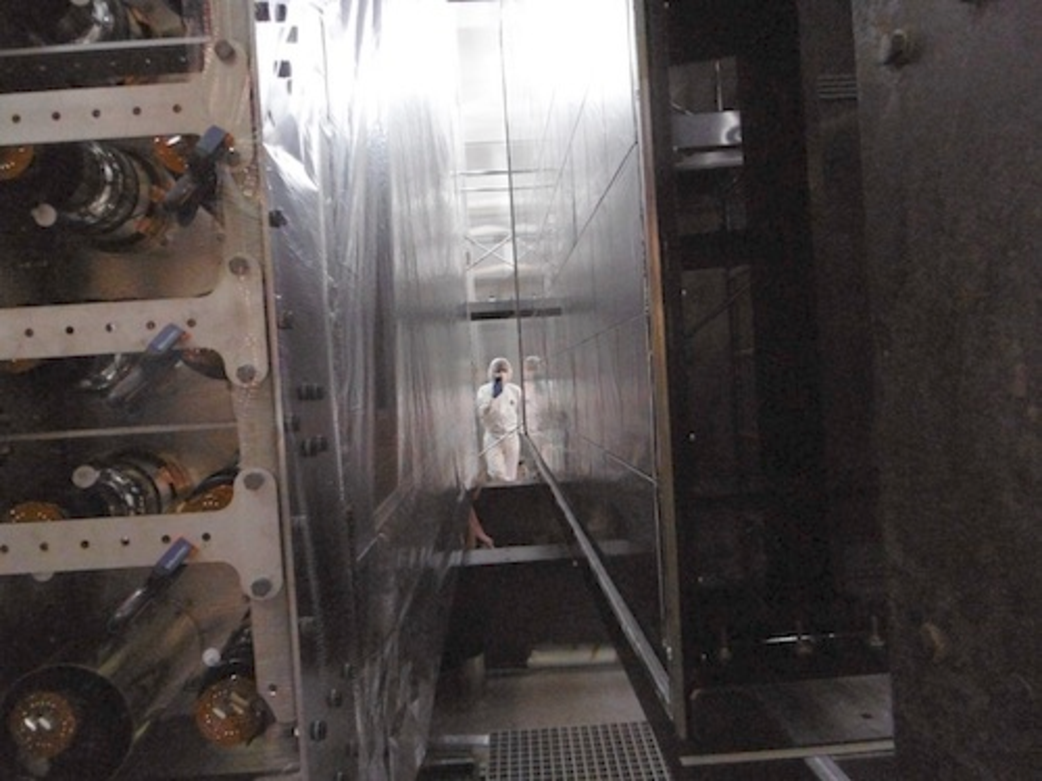
\includegraphics[width=0.7\textwidth]{SNdemonstrator/fig_SNdemonstrator/detector_closing.pdf}
\caption{Last picture of the SuperNEMO demonstrator before closing it, the $22$ November $2018$.
  The picture is taken from one side of the detector, facing the other side.
  We can distinguish on the right the front of one of the two calorimeter main walls, and on the left one of the two tracker chambers.
\label{fig:detector_closing}}
\end{figure}

\section{The SuperNEMO technology}



The SuperNEMO demonstrator, in the manner of NEMO-$3$, combines tracking and calorimetry technologies to record the full event kinematics and measure the particle energies.
It is designed to search for the $\zeronu$ decay which, if observed, would reveal the Majorana nature of the neutrino particle, opening the door of physics beyond the Standard Model, with huge implications for physics research.
The SuperNEMO demonstrator is $6$~meters long, $3$~meters tall and $2$~meters large.
It is the first of the $20$ modules that will make up the final detector.
This unique technology allows the experiment to characterise with a significant performance its own background, placing the detector in the ultra-low background category of experiments.

\subsection{Detection principle}

In Fig.~\ref{fig:demonstrator_scheme} is drawn a simplified scheme of the SuperNEMO demonstrator.
In order to ease the naming of the different areas of the detector, the collaboration has decided to label each part as \emph{French}, \emph{Italian}, \emph{tunnel} or \emph{mountain} sides, given with respect to the orientation of the detector in the underground laboratory.
\begin{figure}[h!]
\centering
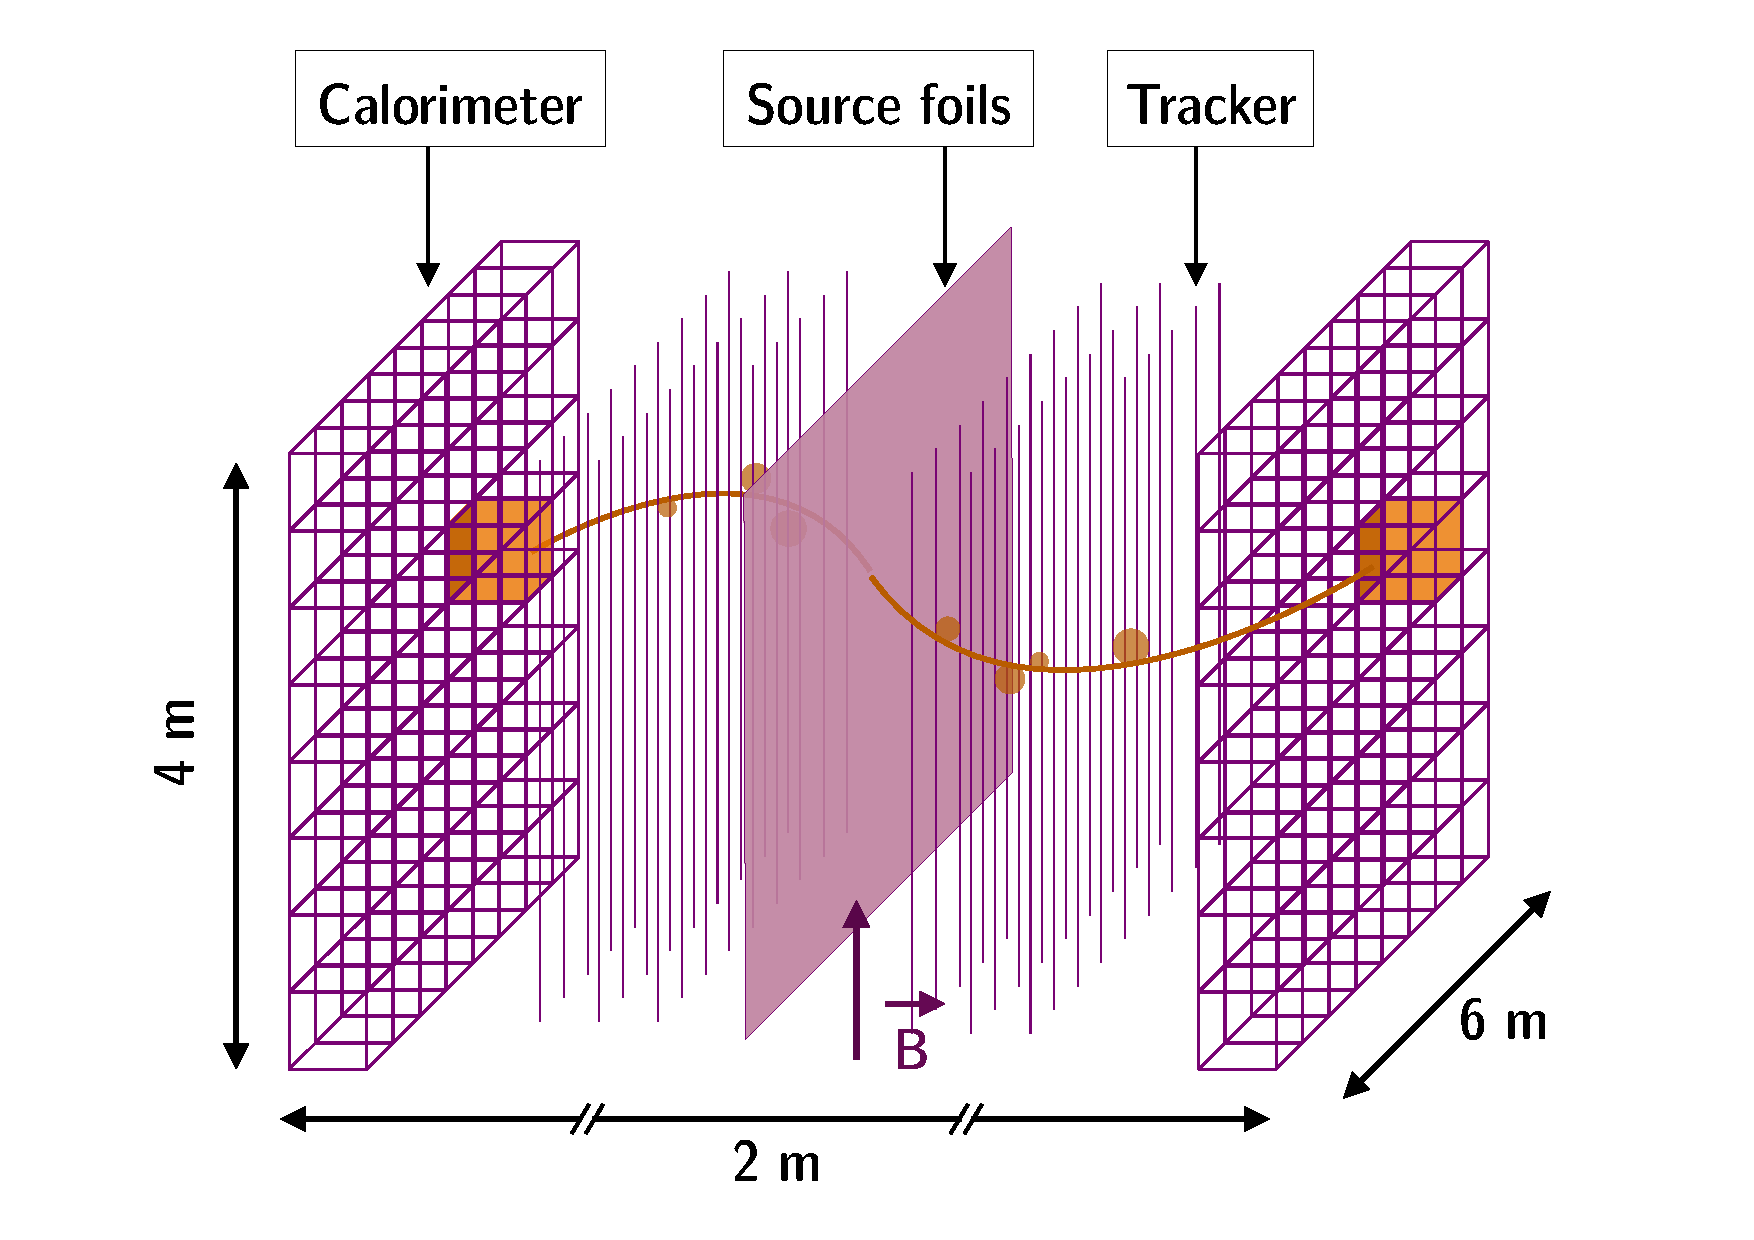
\includegraphics[width=1\textwidth]{SNdemonstrator/fig_SNdemonstrator/demonstrator_sheme.pdf}
\caption{Scheme of an open view of the SuperNEMO demonstrator (not to scale).
  An example of emission from the source foils of two negatively charged particles is drawn.
  Each side of the tracker is labelled as French, Italian, tunnel or mountain side.
\label{fig:demonstrator_scheme}}
\end{figure}

The $\beta\beta$ isotope is distributed within ultra thin foils, at the centre of the detector.
Therefore, for the same detector size, the mass of isotopes studied with this technology is lower than for experiments using liquid scintillators or TPCs.
But as the source is separated from the detection volume, various $\beta\beta$ isotopes can be studied as long as they can be set up in solid thin foils, making this technology very interesting for the search for the $\zeronu$ decay.

An emission of two negatively charged particles\footnote{By convention, a negatively curved track has the curvature of an electron going from the foil to the scintillator main wall.} from the source is also schematised, exiting in opposite directions for this particular case.
The design of SuperNEMO as successive layers of sub-detectors makes it possible to collect a variety of information on the emitted particle.
When crossing the wire chamber, the charged particle ionises the gas, and the arrival time of the signals on the anode and copper rings allows the track reconstruction.
The detector is surrounded by a copper coil, delivering a magnetic field inside the wire chamber.
The few MeV particle trajectories are bent, allowing to discriminate electrons from positrons.
Muons have too much energy for their trajectory to be bent by a magnetic field of this intensity.
The $\alpha$ particles interact too quickly for their track to be curved, but can still be recognised precisely because of this short length (a few cells long).
Therefore, the tracking technology makes it possible to discriminate electrons from positrons (with the trajectory curvature), to identify $\gamma$ particles (corresponding to an energy deposit inside the calorimeter without any associated track), and to tag $\alpha$ particles (characterised by a short delayed track inside the wire chamber).
Thus, although the SuperNEMO energy resolution and detection efficiency are modest compared to germanium or bolometer experiments, it is compensated by the powerful particle identification allowing to identify events coming from natural radioactive decays in dedicated channels.
Particles end up in scintillator blocks, where the collection of deposited charge by a photomultiplier tube allows the incident particle energy measurement.
Electric signals are sent to electronic boards where they are sampled and recorded for off-line analyses.

In addition to the search for the $\zeronu$ decay, the SuperNEMO technology is suitable for the search for other processes like double beta decays to excited states of the daughter nucleus that can be studied in dedicated channels (two-electrons and one/two gamma particles).
Thanks to the topological informations brought by the successive sub-detectors (two single electron energies and emission angle between them), if the $\zeronu$ signal is observed, the SuperNEMO technology would also have the ability to discriminate between different hypothesised underlying mechanisms, allowing to investigate physics beyond the Standard Model.

In the following we describe in detail the successive layers of the SuperNEMO technology, from the $\beta\beta$ emitter source foils to the electronic boards where the signal is sampled.


\subsection{The source foils}

\subsubsection*{Choice of isotope}

There are about $30$ double beta emitters, some of which can be created in laboratory if an enrichment technique exists, for physics research purposes.
The choice of the isotope is directed by several factors and experimental constraints.
Although this choice is specific to each detector, some constraints are common to all $\zeronu$ experiments.
\begin{itemize}
\item The energy transition $\Qbb$: a significant background coming from natural radioactivity is the $2.615$~MeV-$\gamma$ emitted after the Thallium-$208$ (\Tl) $\beta$ disintegration.
  Also, Bismuth-$214$ (\Bi) isotope disintegrations have a high available energy with ${Q_{\beta}=3.27}$~MeV.
  Therefore, a high $\Qbb$ would help to guaranty the experiment to be free from radioactive background.
\item The phase space factor and the nuclear matrix elements: as described in Chapter~\ref{ch:pheno}, the $\zeronu$ half-life depends on these two parameters.
  The higher they are, the more signal events are expected for a given data acquisition time.
  Unfortunately, the uncertainties that exist on nuclear matrix element calculations prevent from reaching a clear conclusion on the isotope choice.
\item The $\twonu$ half-life: this process represents an unavoidable background for the search for $\zeronu$.
Then, the higher the half-life of this process, the less $\twonu$ events are expected.
\item The natural abundance: the higher it is, the more we can produce substantial quantities of the enriched isotope.
\item Ease of enrichment: although it is not a measurable quantity as previous requirements, known purification techniques must be applicable to the isotope considered to reach high quantities of $\beta\beta$ emitter.
\end{itemize}
In Tab.~\ref{tab:bb_isotopes} are given these characteristics for some of the $\beta\beta$ emitters used for current $\zeronu$ searches.
\Se\ was chosen for SuperNEMO because of its high transition energy, and preferred to \Mo\ because of its higher $\twonu$ half-life (by a factor $\sim13$).
Its nuclear phase space factor and natural abundance are satisfying and its enrichment is feasible using classical technique (centrifugation).
\begin{table}[h!]
\centering
\begin{tabular}{|c|c|c|c|c|c|}
\hline
Isotope & $Q_{\beta\beta}$ (MeV) & $G_{0\nu}$ ($10^{-15}$ y$^{-1}$) & $T^{2\nu}_{1/2}$ (y) & $\eta$ ($\%$) \\
\hline
\hline
$^{48}$Ca & $4.273$ & $24.81$ & $6.37\times 10^{19}$ & $0.187$ \\
$^{76}$Ge & $2.039$ & $2.363$ & $1.926\times 10^{21}$ & $7.8$ \\
$^{82}$Se & $2.995$ & $10.16$ & $9.6\times 10^{19}$ & $9.2$ \\
$^{96}$Zr & $3.350$ & $20.58$ & $2.35\times 10^{19}$ & $2.8$ \\
$^{100}$Mo & $3.035$ & $15.92$ & $6.93\times 10^{18}$ & $9.6$ \\
$^{116}$Cd & $2.809$ & $16.70$ & $2.8\times 10^{19}$ & $7.6$ \\
$^{130}$Te & $2.530$ & $14.22$ & $6.9\times 10^{20}$ & $34.5$ \\
$^{136}$Xe & $2.458$ & $14.58$ & $2.165\times 10^{21}$ & $8.9$ \\
$^{150}$Nd & $3.367$ & $63.03$ & $9.11\times 10^{18}$ & $5.6$ \\
\hline
\end{tabular}
\caption{$\beta\beta$ emitters used in current $\zeronu$ experiments.
$\Qbb$, phase space factors, $\twonu$ half-lives and natural abundances are given.
\label{tab:bb_isotopes}}
\end{table}

\subsubsection*{Source foils production}

The \Se\ isotope is enriched and purified by the ITEP laboratory in Russia.
Two purification techniques have been employed, given in Tab.~\ref{tab:Se_purification}.
Approximate isotope quantities are given for each technique.
About $6.5$~kg of \Se\ powder have been produced and purified.
The \Se\ is then ground to a fine powder ($50~\mu$m grains) and mixed with a radio-pure glue.
\begin{table}[h!]
\centering
\begin{tabular}{|c|c|c|}
\hline
Enrichment technique & \Se\ quantity (kg) & Number of foils \\
\hline
\hline
Double distillation & $\sim2$+$1.5$ & $\sim11$+$8$\\
Reverse chromatography & $\sim3$ & $\sim15$\\
\hline
\end{tabular}
\caption{Different purification techniques and corresponding approximate quantities of \Se\ isotope produced.
Two batches of \Se\ have been produced through double distillation.
\label{tab:Se_purification}}
\end{table}

To shape the \Se\ powder into the final SuperNEMO source foils, two distinct designs have been tested, one by ITEP and the other by the LAPP laboratory in Annecy (Fig.~\ref{fig:foils_design}).
\begin{itemize}
\item ITEP implemented the same technique as for NEMO-$3$ source foils, by smearing the \Se+glue mixture between two $12~\mu$m thick Mylar backing films, creating $3$~meters long foils.
  The Mylar is perforated by irradiation, allowing the mixture to dry and better adhere to the film.
  However this technique could contaminate the source, which encouraged the development of an alternative technique.
\item The LAPP team split up the foils in several pads: two Mylar sheets are heat welded together to host the several pads.
\end{itemize}
The principal interest in designing the sources that thin is to maximise the chances of the electrons produced inside the source to escape it, to be detected by the successive sub-layers.
Moreover, thinner sources reduce electron energy losses inside the source, and thus their fluctuations, which contributes to the improvement of the detector global energy resolution.
In addition, the collaboration made this design choice in order to leave the possibility of easy isotope change in the future.
Finally, $6.23$~kg of \Se\ have been distributed into $34$ source foils each of them measuring $135.5\times2700$~mm.
The thickness of the produced sources were precisely measured at $300~\mu$m by the collaboration.
\begin{figure}[h!]
\centering
\begin{subfigure}[t]{0.49\textwidth}
\centering
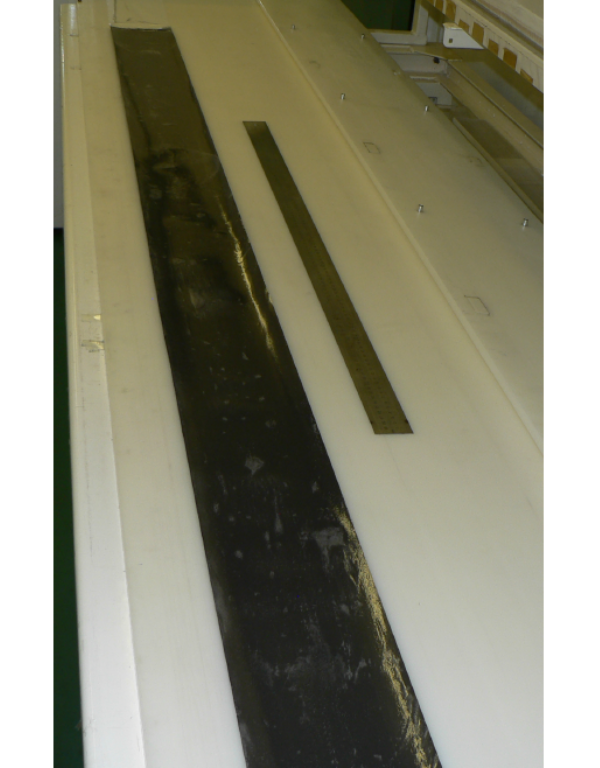
\includegraphics[width=0.9\textwidth]{SNdemonstrator/fig_SNdemonstrator/ITEP_source_foils.png}
\captionsetup{justification=centering}
\caption{ITEP style foils.
\label{subfig:ITEP_foils}}
\end{subfigure}
\hfill
\begin{subfigure}[t]{0.49\textwidth}
\centering
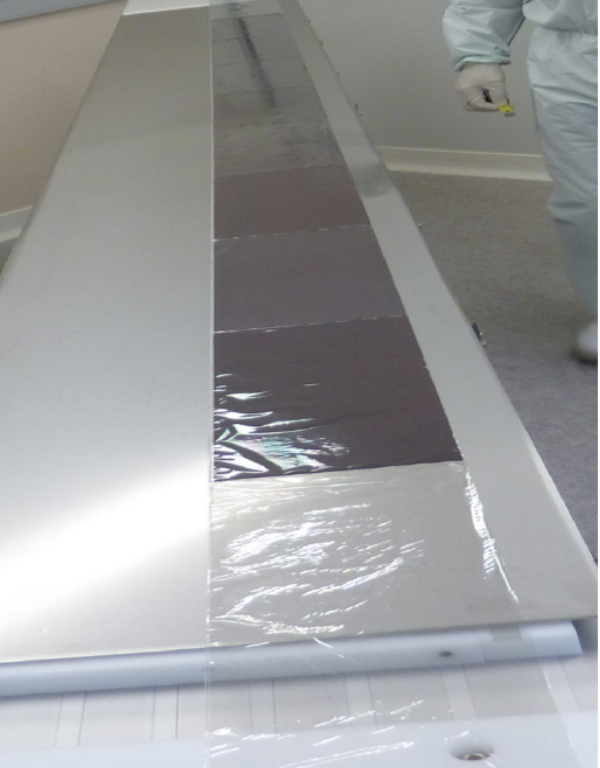
\includegraphics[width=0.9\textwidth]{SNdemonstrator/fig_SNdemonstrator/LAPP_source_foils.png}
\captionsetup{justification=centering}
\caption{LAPP style foils.
\label{subfig:LAPP_foils}}
\end{subfigure}
\caption{Two designs of source foils, ITEP (left) and LAPP (right).
\label{fig:foils_design}}
\end{figure}

\subsubsection*{Source foils installation}
The $24$ September $2018$, each strip was fasten to a frame measuring $4.857$~meters large and $2.7$~meters high.
The original plan was to place the ITEP sources next to each other and to do the same for the LAPP sources.
Unfortunately, some of the sources had to be relocated because of source shape issues (in particular, some sources were in contact with the Bismuth calibration sources described in Sec.~\ref{subsec:calib}).
The final position decided for the source foils are pictured in Fig.~\ref{fig:source_foils_installation}, where we can see the alternation of ITEP and LAPP sources.
ITEP sources appear slightly curved on the picture, what probably happened during the glue drying step.
We can also distinguish the presence of the vertical wires of the tracker before the sources, discussed in next sub-section.
Each source curvature have been precisely measured using a laser tracking system, for a future precise description of the sources geometry and its integration in the simulation software.
I was part of the team that carried out the first curvature measurements right after sources integration in Modane.
\begin{figure}[h!]
\centering
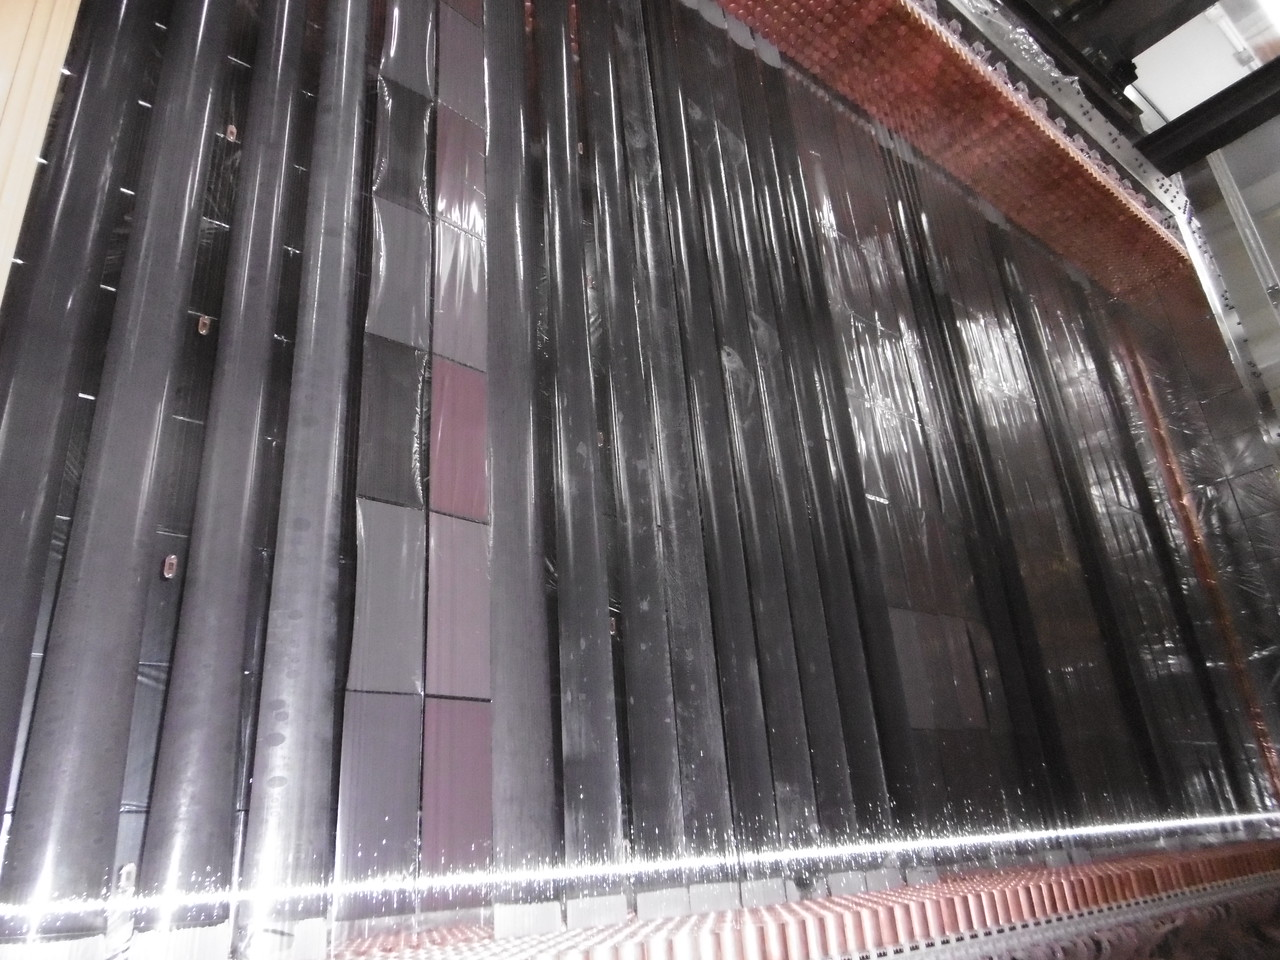
\includegraphics[width=0.9\textwidth]{SNdemonstrator/fig_SNdemonstrator/sources_installed.jpg}
\caption{Source foils final position.
  The ITEP foils (one-piece long foils) and LAPP foils (divided in pads) are easily distinguishable.
  \label{fig:source_foils_installation}}
\end{figure}


\subsection{The tracker}
\label{subsec:tracker}

The tracker is a detector aiming at measuring the charged particle three-dimensional trajectories, through their electromagnetic interaction with the gas filling the tracking chamber.
This sub-detector allows for efficient background rejection through the identification of particles, by making sure the event is composed of exactly two electrons.
The reconstruction of the vertices on the source makes it possible to identify highly contaminated areas, the so-called \emph{hot spots} of the experiment, and to reject them with appropriate cut-offs.
The SuperNEMO tracker is divided into two halves, one on each side of the source frame, to measure particles exiting from it in all possible directions.
These are two drift chambers filled with a gas mixture and operating in Geiger mode.

\subsubsection*{Geiger counters}

In Fig.~\ref{fig:geiger_avalanche} is schematised the basic operation principle of a Geiger cell.
When a particle goes through the gas in which the cell is immersed, it ionises it all along its path, creating positive charges on one hand (heavy ions) and negative on the other hand (electrons).
A high electric potential is applied, allowing the freed electrons to drift towards the anodic wire, and the ions towards the field wire.
When ionisation electrons come close to the anodic wire, the electric field becomes so high that the accelerated electrons can themselves ionise the gas, creating electronic avalanches until the wire is reached.
Other avalanches are created all along the anode wire by de-excitation and recombination of UV photons.
The Geiger mode is reached when the avalanches created by the electrons are saturated: increasing the voltage does not increase the collected charge.
This is the so-called \emph{Geiger plateau}, which provides a very high detection efficiency ($>99$\%).
The longitudinal position is obtained with the time needed for these avalanches to reach both ends of the wire.
\begin{figure}[h!]
\centering
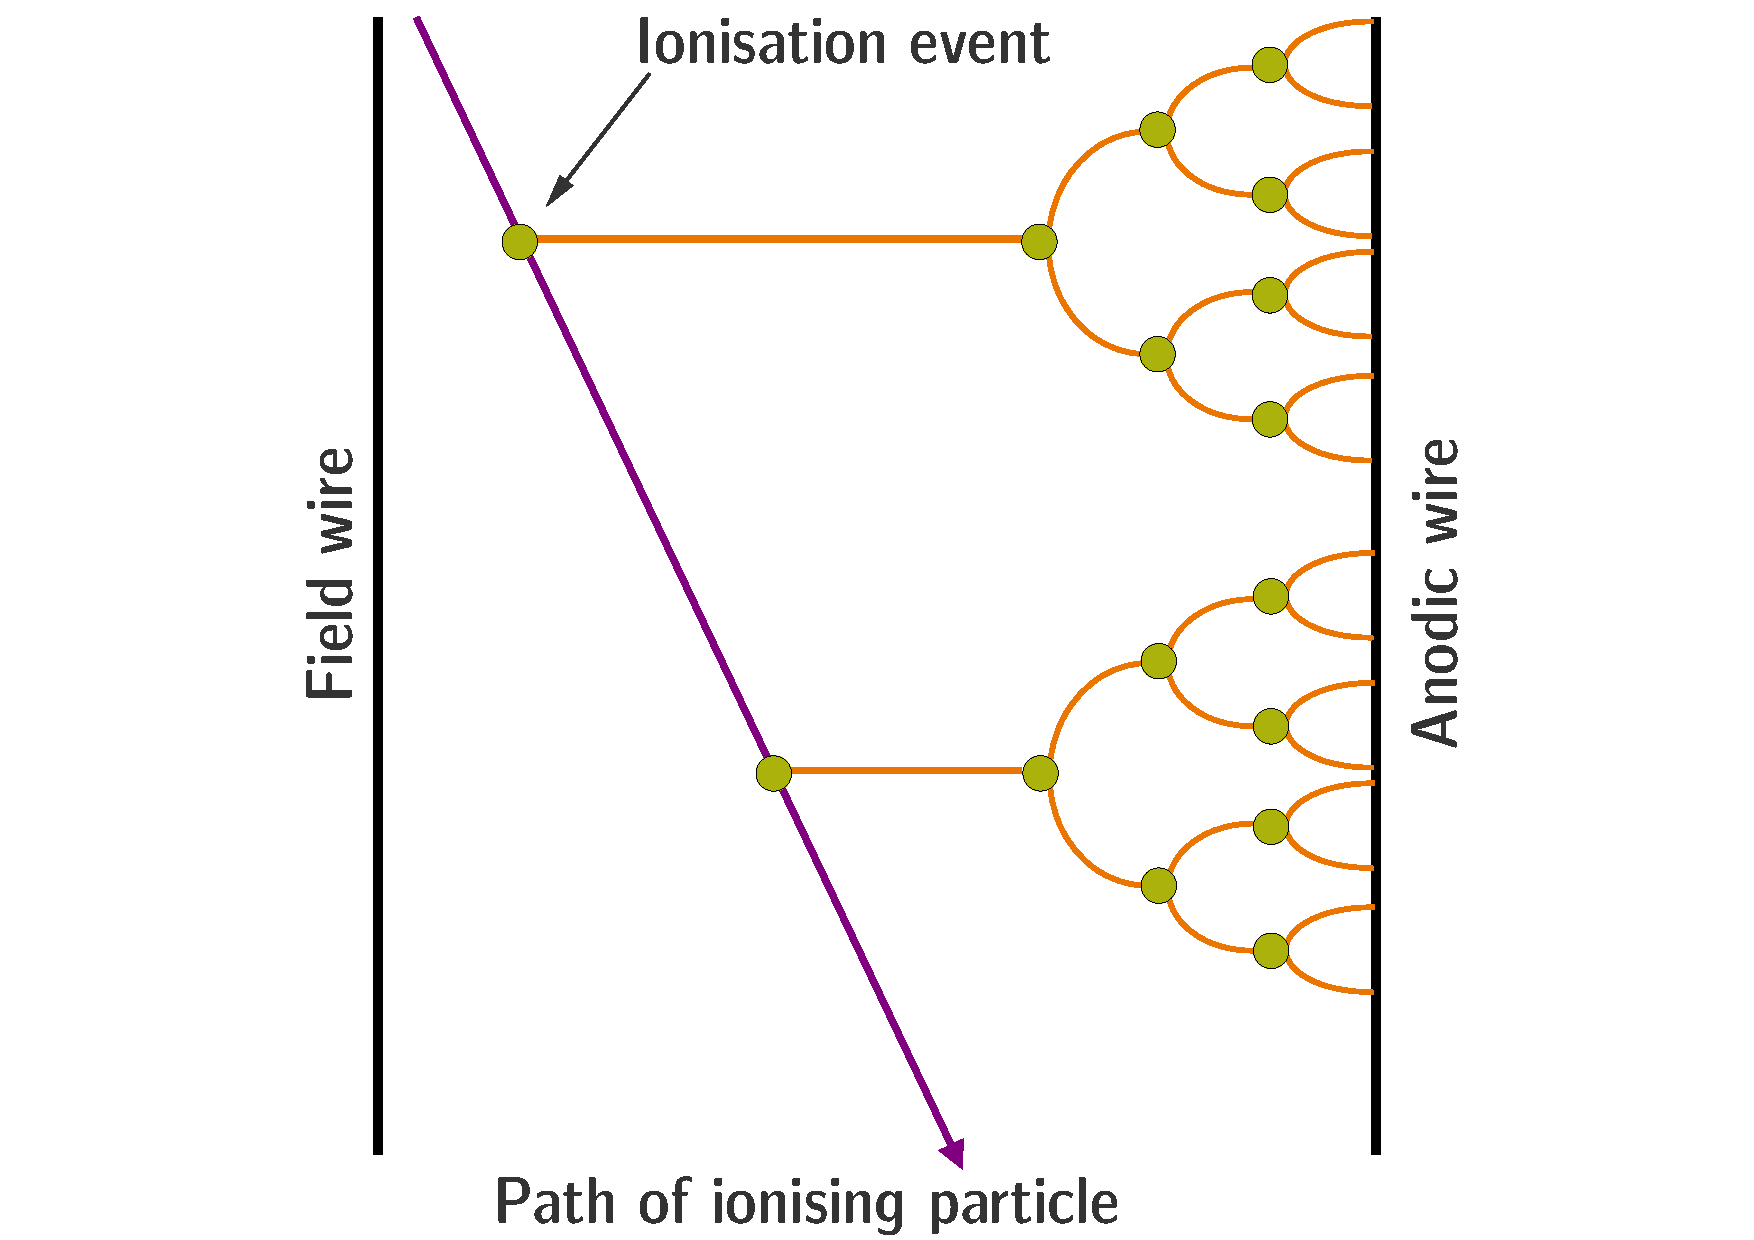
\includegraphics[width=0.7\textwidth]{SNdemonstrator/fig_SNdemonstrator/geiger_avalanche.pdf}
\caption{The principle of a Geiger cell illustrated with one central anodic wire and one field wire.
  Electrons (orange) drift to the anodic wire.
\label{fig:geiger_avalanche}}
\end{figure}


\subsubsection*{SuperNEMO cells}

A minimal amount of material is required inside the tracker chambers, for the particles to freely cross it with limited energy losses and reduced multiple scatterings.
However, a minimal distance between the tracker wires is required in order to efficiently collect the charges coming from gas ionisation.
Taking into account the tracker spatial resolution needs and the constraints on gas mixture composition, the decision was made to design Geiger cells as in Fig.~\ref{fig:SN_geiger_cell}, with one central anodic wire (stainless steel, $40\mu$m in diameter) and $12$ surrounding field wires (stainless steel, $50\mu$m in diameter).
Each cell has a diameter of $4.4$~cm.
Two copper rings, of $4$~cm diameter and $4$~cm long, are placed on both ends of each cell, allowing the cessation of the avalanches.
In total, the tracker chamber is composed of $2034$ Geiger cells of $3$~m long, divided in $9\times113$ layers, parallel to the source strips.
The minimal distance between the ionising particle and the anode, called \emph{radial distance}, is given by the anodic signal.
The interaction point along the cell axis, called \emph{longitudinal position}, is obtained with the time needed for the avalanches to reach both ends of the cell.
In the SuperNEMO operating conditions, a few micro seconds elapse between the creation of the first ionisation electron and the creation of the first avalanche, after which the avalanche is expected to spread through a cell in about $40~\mu$s~\cite{docdb:ashwin2015}.
The final reconstructed times at which a charge particle passes nearby successive tracker cells are defined using the particle arrival time in the calorimeter as a reference.
\begin{figure}[h!]
\centering
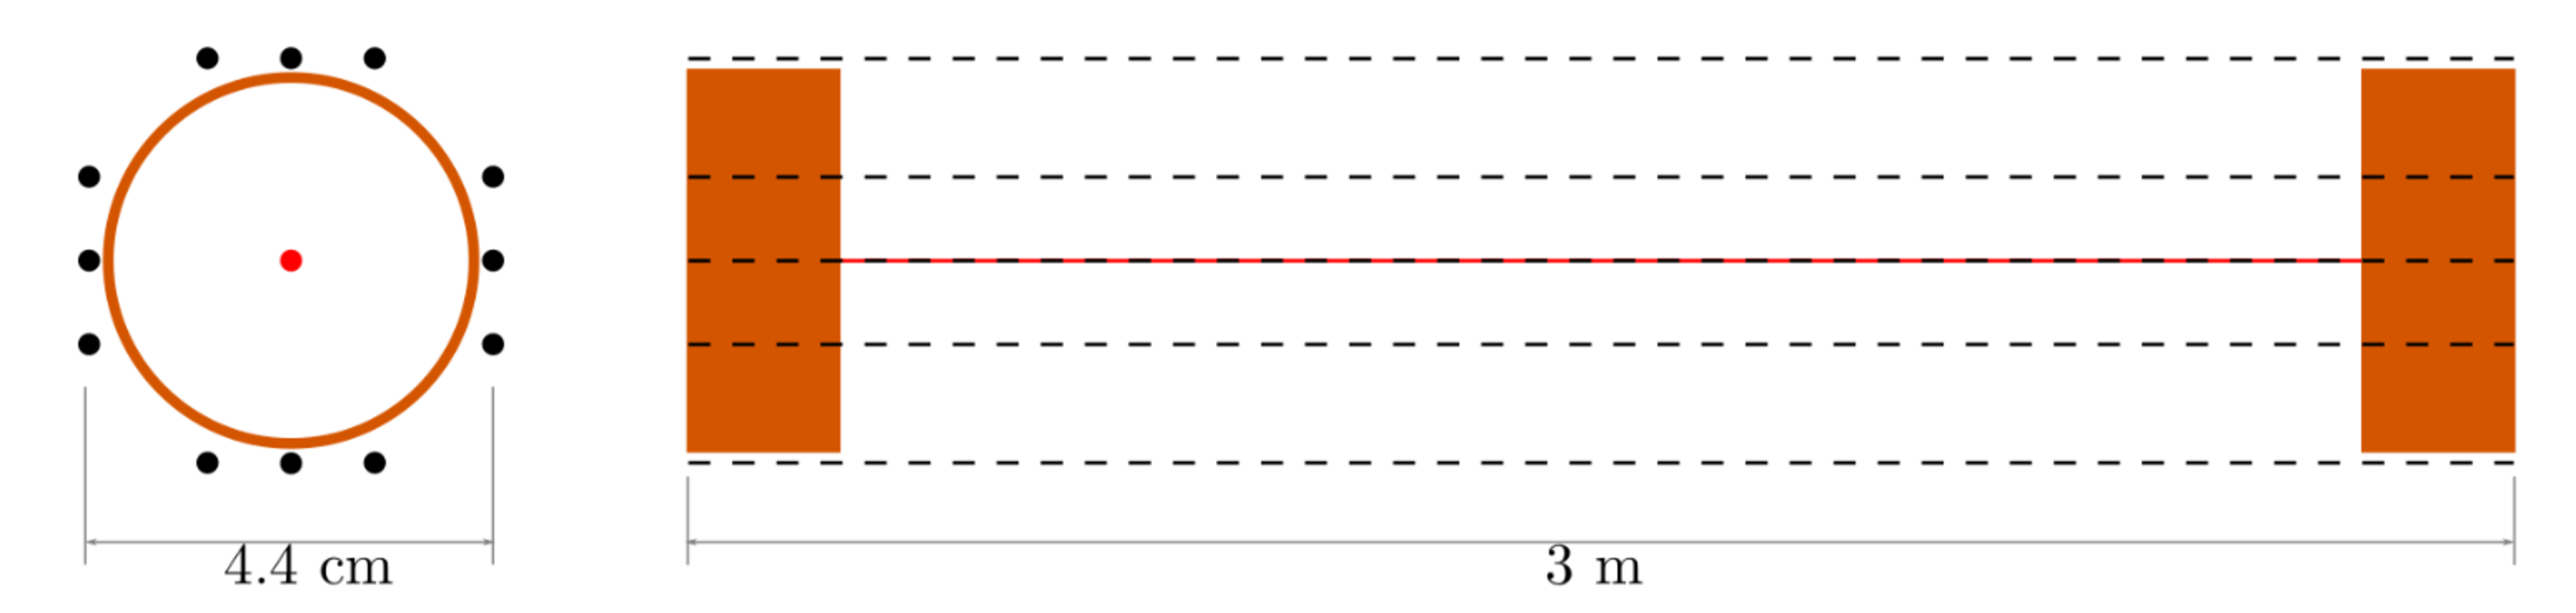
\includegraphics[width=1\textwidth]{SNdemonstrator/fig_SNdemonstrator/geiger_cell.pdf}
\caption{Sketch of a SuperNEMO Geiger cell, in transverse view (left) and side view (right, the sketch is rotated of $90^{\circ}$ as the Geiger cells are vertical in the SuperNEMO demonstrator).
  The anodic central wire is represented at the centre in red.
  Field wires, in black, surround it to form $4.4$~cm large and $3$~m long Geiger cells.
  On the right the copped rings are also represented by orange stripes at both ends of the wires.
\label{fig:SN_geiger_cell}}
\end{figure}

As we said, the behaviour of a Geiger cell depends on the voltage applied.
For the SuperNEMO cells, the Geiger plateau is located around $1800$~V and is $\sim300$~V-wide~\cite{docdb:tracker_review2014}.
However, the exact voltage to be applied to each cell depends on their individual properties, and will have to be determined and set up after the tracker commissioning phase.


\subsubsection*{Gas mixture}

The tracker gas composition is decisive for the wire chamber operation.
For the SuperNEMO demonstrator, it is composed as follows:
\begin{itemize}
\item Helium is the main component, which is ionised by incident radiations.
  As an inert gas, it does not react with the detector sensitive parts.
\item Argon ($1$\%) enhances the propagation of avalanches along the anode wires thanks to its lower ionisation energy.
\item Ethanol ($4$\%) is used as a quenching agent, stopping the successive discharges.
\end{itemize}
This gas composition guarantees a medium with a low $Z$ number in order to minimise the energy losses and particle multiple scatterings.

\subsubsection*{Tracker installation}

Each of the tracker halves is itself divided into two C-sections (named in this way according to the C-shape of each section) assembled at UCL’s Mullard Space Science Laboratory.
They were delivered individually and integrated in Modane to form the two tracker chambers.
In Fig.~\ref{fig:me_tracker} is given a picture of the tracker after its integration to the detector.
The bottom copper rings are noticeable and indicate the presence of the Geiger cells whose wires are too thin to be visible on the picture.
After installation, some meticulous work were achieved to remove few wires damaged during transport.
\begin{figure}[h!]
\centering
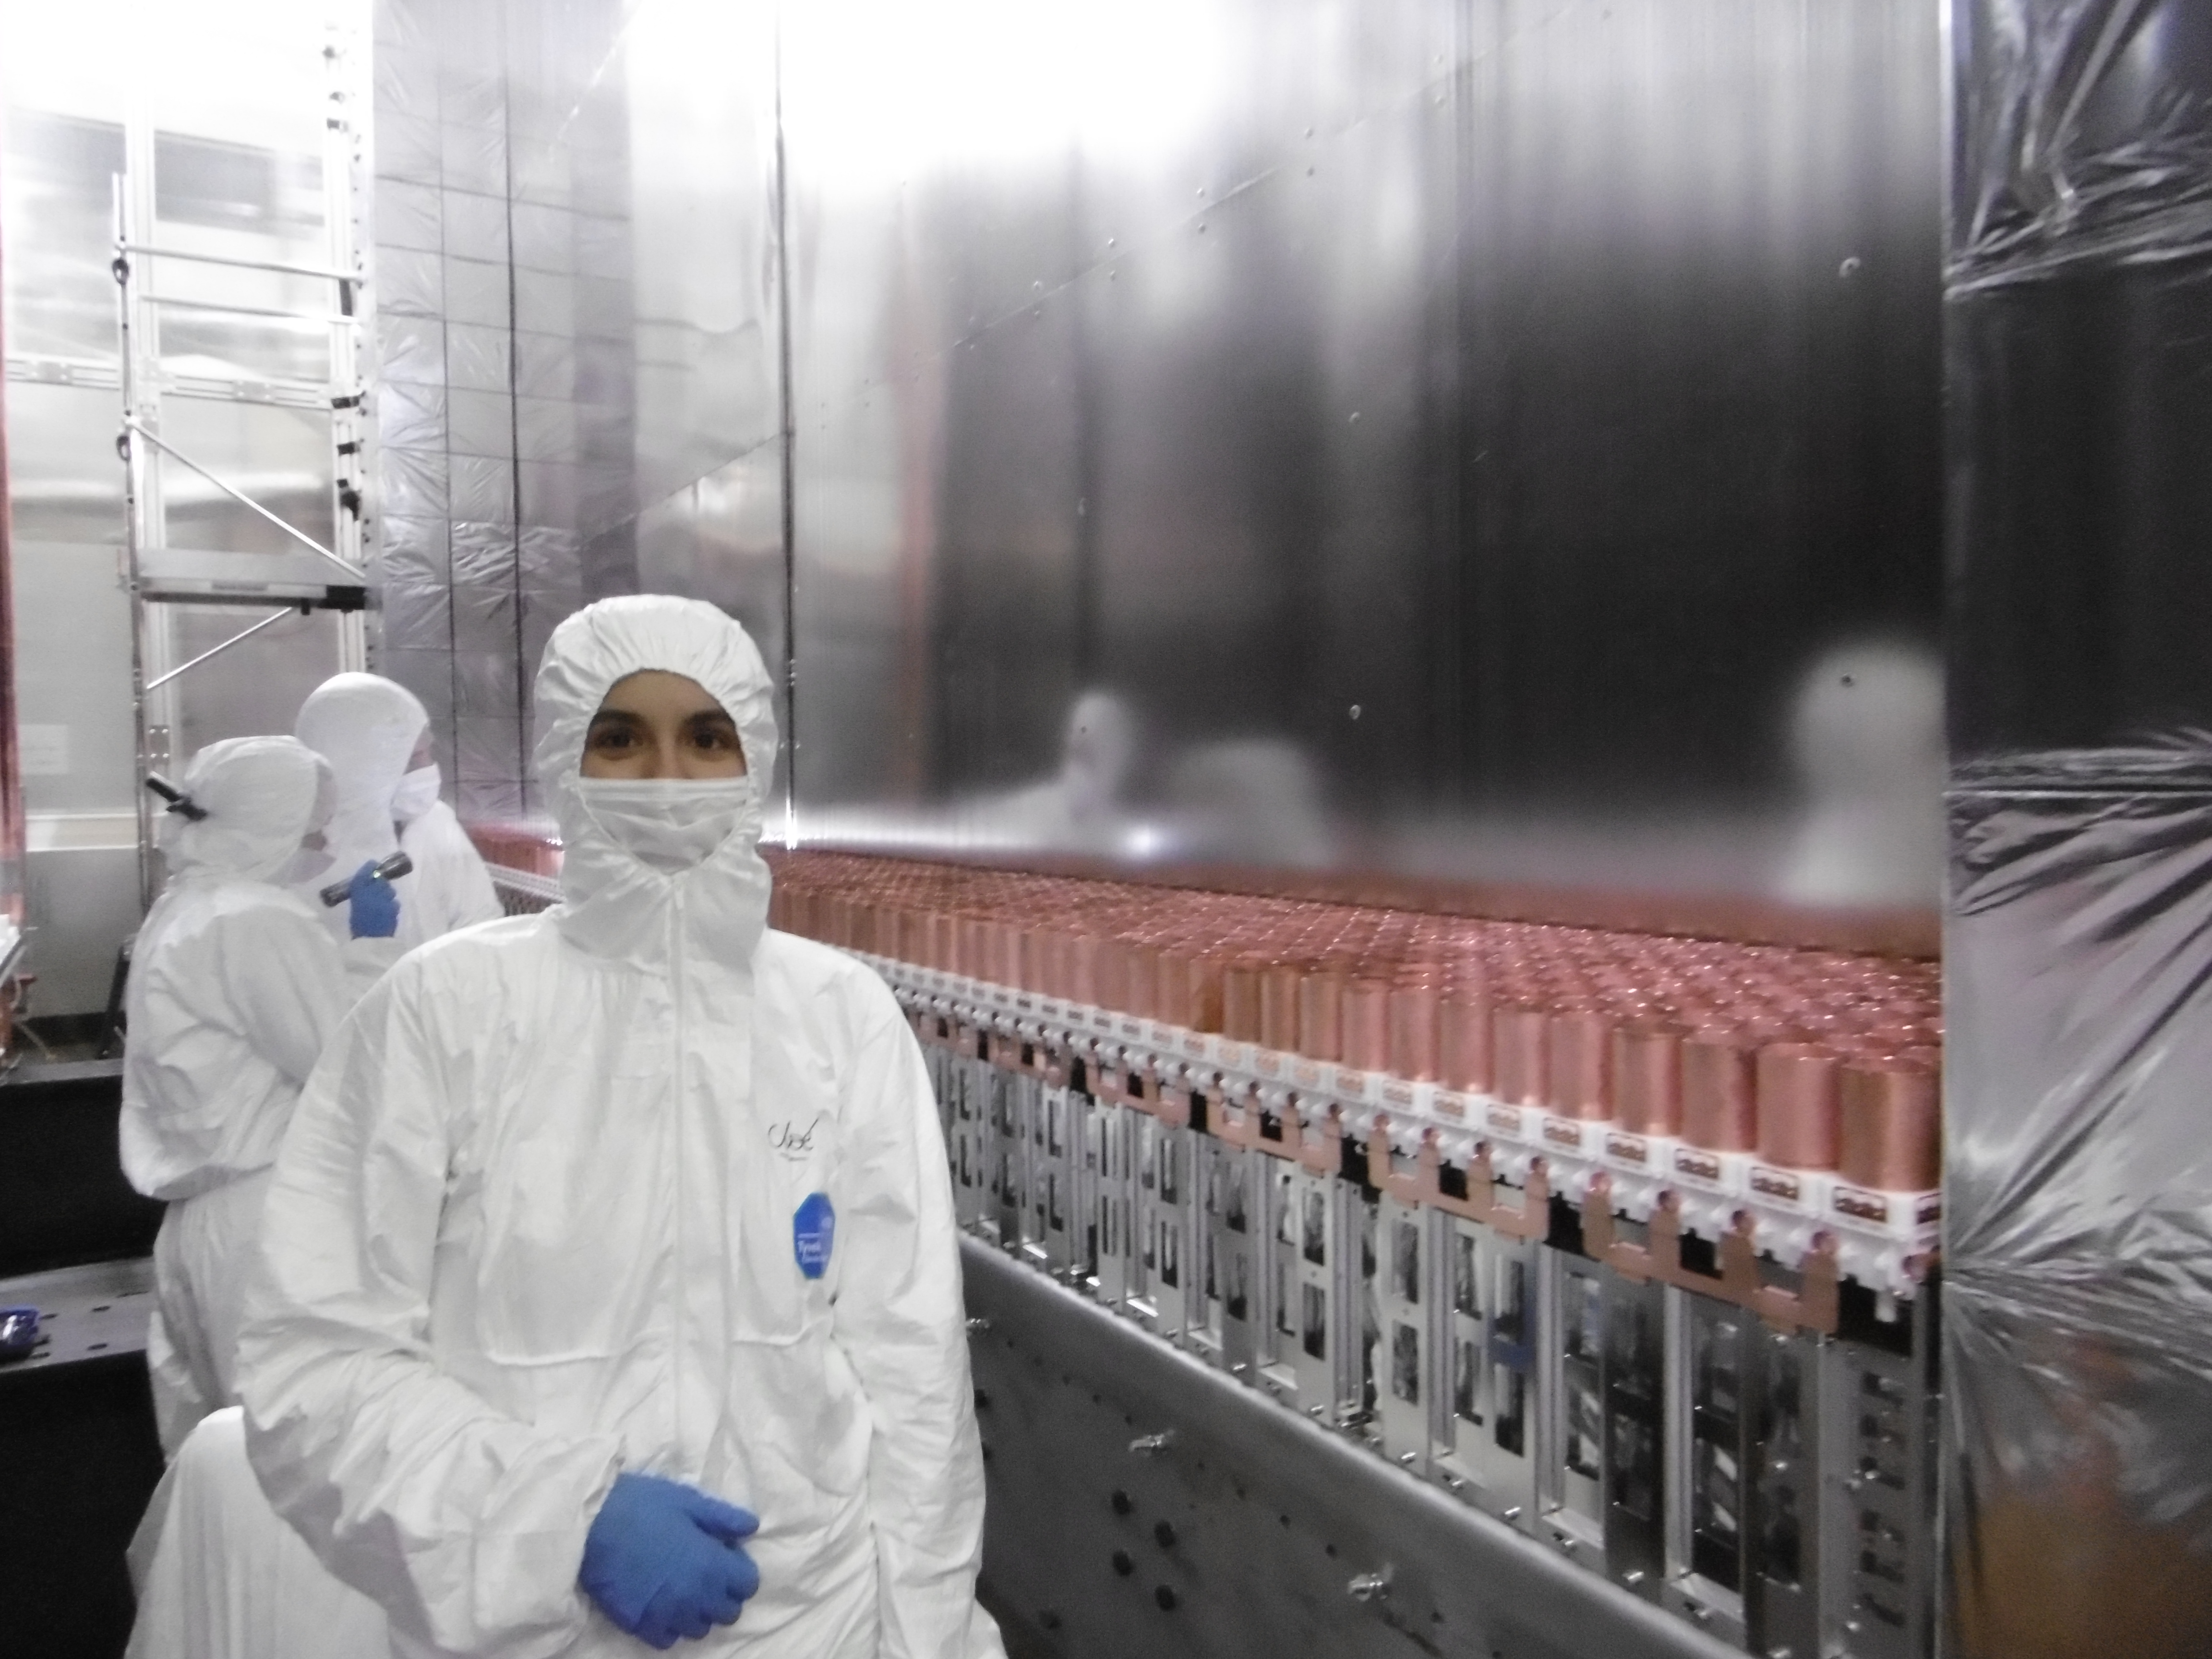
\includegraphics[width=0.9\textwidth]{SNdemonstrator/fig_SNdemonstrator/tracker_selfie.jpg}
\caption{Inside view of the tracker (with me standing in the foreground), before detector closing, on the day of the wire check, looking for possible broken wires at the base of the copper rings.
\label{fig:me_tracker}}
\end{figure}

\subsubsection*{Gas sealing}

A constant over-pressure is kept inside the tracker, which is imperative to maintain the right gas mixture, without infiltration of outside air.
Indeed, if atmospheric air enters the gas detector, its properties can be disturbed.
For example, the quenching may become too strong and the signal can not be properly transmitted through the gas.
Therefore, once the tracker was integrated into the detector, a huge effort was achieved by the entire collaboration to seal it.
In the case of SuperNEMO, it is also necessary that the detector is sealed to prevent helium from escaping and penetrating into the vacuum tubes of the PMs.
As a PhD student in the collaboration, I had the opportunity to participate in much of this work.
The different techniques used to seal the detector are discussed in detail in Sec.~\ref{subsec:sealing}.

The tracking part of the demonstrator enters the commissioning phase in November $2020$.
Among other, each cell will have to be characterised, and is expected to have a $0.7$~mm radial and $1$~cm vertical spatial resolutions.


\subsection{The calorimeter}
\label{subsec:SN_calo}

The $\twonu$ is an irreducible background for the $\zeronu$ decay.
Both of them have the same signature in the tracker, with the emission of two electrons from the source foils.
The only way for the SuperNEMO technology to distinguish them is to measure the two electrons individual energies.
In order to achieve the target sensitivity, the calorimeter R\&D program for SuperNEMO has covered three main areas of study: geometry, energy resolution and radiopurity.
The two firsts are discussed in this sub-section, while the last one is detailed in Sec.~\ref{subsec:SNbkg_internal}~and~\ref{subsec:SNexternal_bkg}.
\begin{itemize}
\item As shown in Fig.~\ref{fig:demonstrator_scheme}, the SuperNEMO calorimeter is segmented to measure the individual energies.
A compromise has been reached between a high granularity and the minimisation of dead zones.
Also, mainly for financial considerations, the number of electronic channels had to remain reasonable.
\item The lower the energy resolution, the more $\twonu$ and $\zeronu$ energy spectra can be discriminated.
In order to achieve the target sensitivity, the energy resolution of the SuperNEMO calorimeter is required to be around $8$\%~FWHM at $1$~MeV for electrons.
The requirement for the time resolution is set to be ${\sigma_{t}=400}$~ps at $1$~MeV for external background rejection purposes (to discriminate between two-electron internal events from those that originate outside of the detector and then cross its active volume to imitate $\zeronu$ events).
\end{itemize}
Each individual optical module (OM) is made of the association between two sub-detectors, a scintillator and a photomultiplier (PM).


\subsubsection*{Scintillators}

The material chosen for the SuperNEMO scintillators is an organic, polystyrene-based material, doped with $0.05$\% of POPOP (1.4-bis(5-phenyloxazol-2-yl) benzene), a scintillator used as a wavelength shifter, and $1.5$\% of p-Terphenyl (p-TP), a secondary wavelength shifter.
This composition fulfils the requirements of high light yield, low electron back-scattering (because of its low Z), high radiopurity, good timing and a relatively low cost.
Four main geometries have been considered for the scintillator blocs during the R\&D phase, all presented in Fig.~\ref{fig:scint_shape}.
What all these forms have in common is that they can be stacked to form a compact active detection volume, thanks to their entrance face shapes.
Tapered geometries have been considered in order to reduce the amount of material.
The hexagonal shape was designed to get closer to a cylindrical shape and thus to limit edge effects on light propagation inside the scintillator.
However, Monte-Carlo simulations and measurements were carried out, showing the best energy resolutions are reached for hexagonal and cuboid $256\times256$~mm$^{2}$ shapes.
As these two geometries give similar energy resolution results, the cuboid block has been chosen for the final design to ease the manufacturing.
A two dimensional drawing, as well as a picture of a cuboid scintillator is given in Fig.~\ref{fig:scintillator_design}.
The scintillator block is hollowed out to receive the photomultiplier bulb.
%%To enhance the external gammas rejection by enlarging their detection in the scintillator, the
%%... blocks are designed thicker
The SuperNEMO scintillator blocks are designed thicker compared to that of NEMO-$3$ to enhance the $\gamma$ detection and thus improve the background rejection.
In order to increase the collection light efficiency, each scintillator block is wrapped in radio-pure Teflon (on its sides) and aluminised Mylar (on its sides and front face).
The latter also protects the scintillators against the UV photons coming from the tracker chamber and other surrounding optical modules.
\begin{figure}[!h]
\centering
\begin{subfigure}[t]{0.2\textwidth}
  \centering
  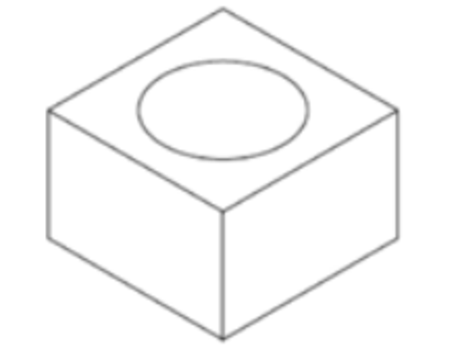
\includegraphics[height=0.8\textwidth]{SNdemonstrator/fig_SNdemonstrator/square_shape.pdf}
  \captionsetup{justification=centering}
  \caption{Cuboid shape $256\times256$~mm$^{2}$.
    \label{subfig:square_shape}}
\end{subfigure}
\hfill
\begin{subfigure}[t]{0.2\textwidth}
  \centering
  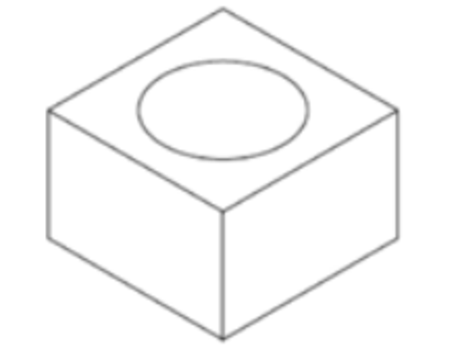
\includegraphics[height=0.8\textwidth]{SNdemonstrator/fig_SNdemonstrator/square_shape.pdf}
  \captionsetup{justification=centering}
  \caption{Cuboid shape $308\times308$~mm$^{2}$.
    \label{subfig:square_shape}}
\end{subfigure}
\hfill
\begin{subfigure}[t]{0.2\textwidth}
  \centering
  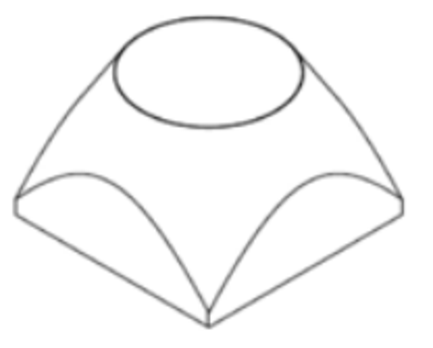
\includegraphics[height=0.8\textwidth]{SNdemonstrator/fig_SNdemonstrator/pyramid_shape.pdf}
  \captionsetup{justification=centering}
  \caption{Tapered shape $308\times308$~mm$^{2}$.
    \label{subfig:square_shape}}
\end{subfigure}
\hfill
\begin{subfigure}[t]{0.2\textwidth}
  \centering
  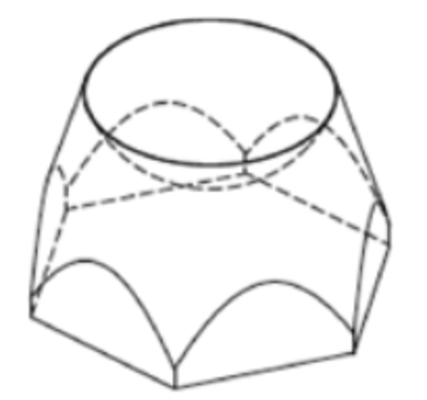
\includegraphics[height=0.8\textwidth]{SNdemonstrator/fig_SNdemonstrator/bee_shape.pdf}
  \captionsetup{justification=centering}
  \caption{Hexagonal shape \o{}~$276$~mm.
    \label{subfig:square_shape}}
\end{subfigure}
\caption{Scintillator shapes considered for the SuperNEMO demonstrator.
  The first one had been selected.
  \label{fig:scint_shape}}
\end{figure}
\begin{figure}[!h]
  \centering
  \begin{subfigure}[t]{0.49\textwidth}
    \centering
    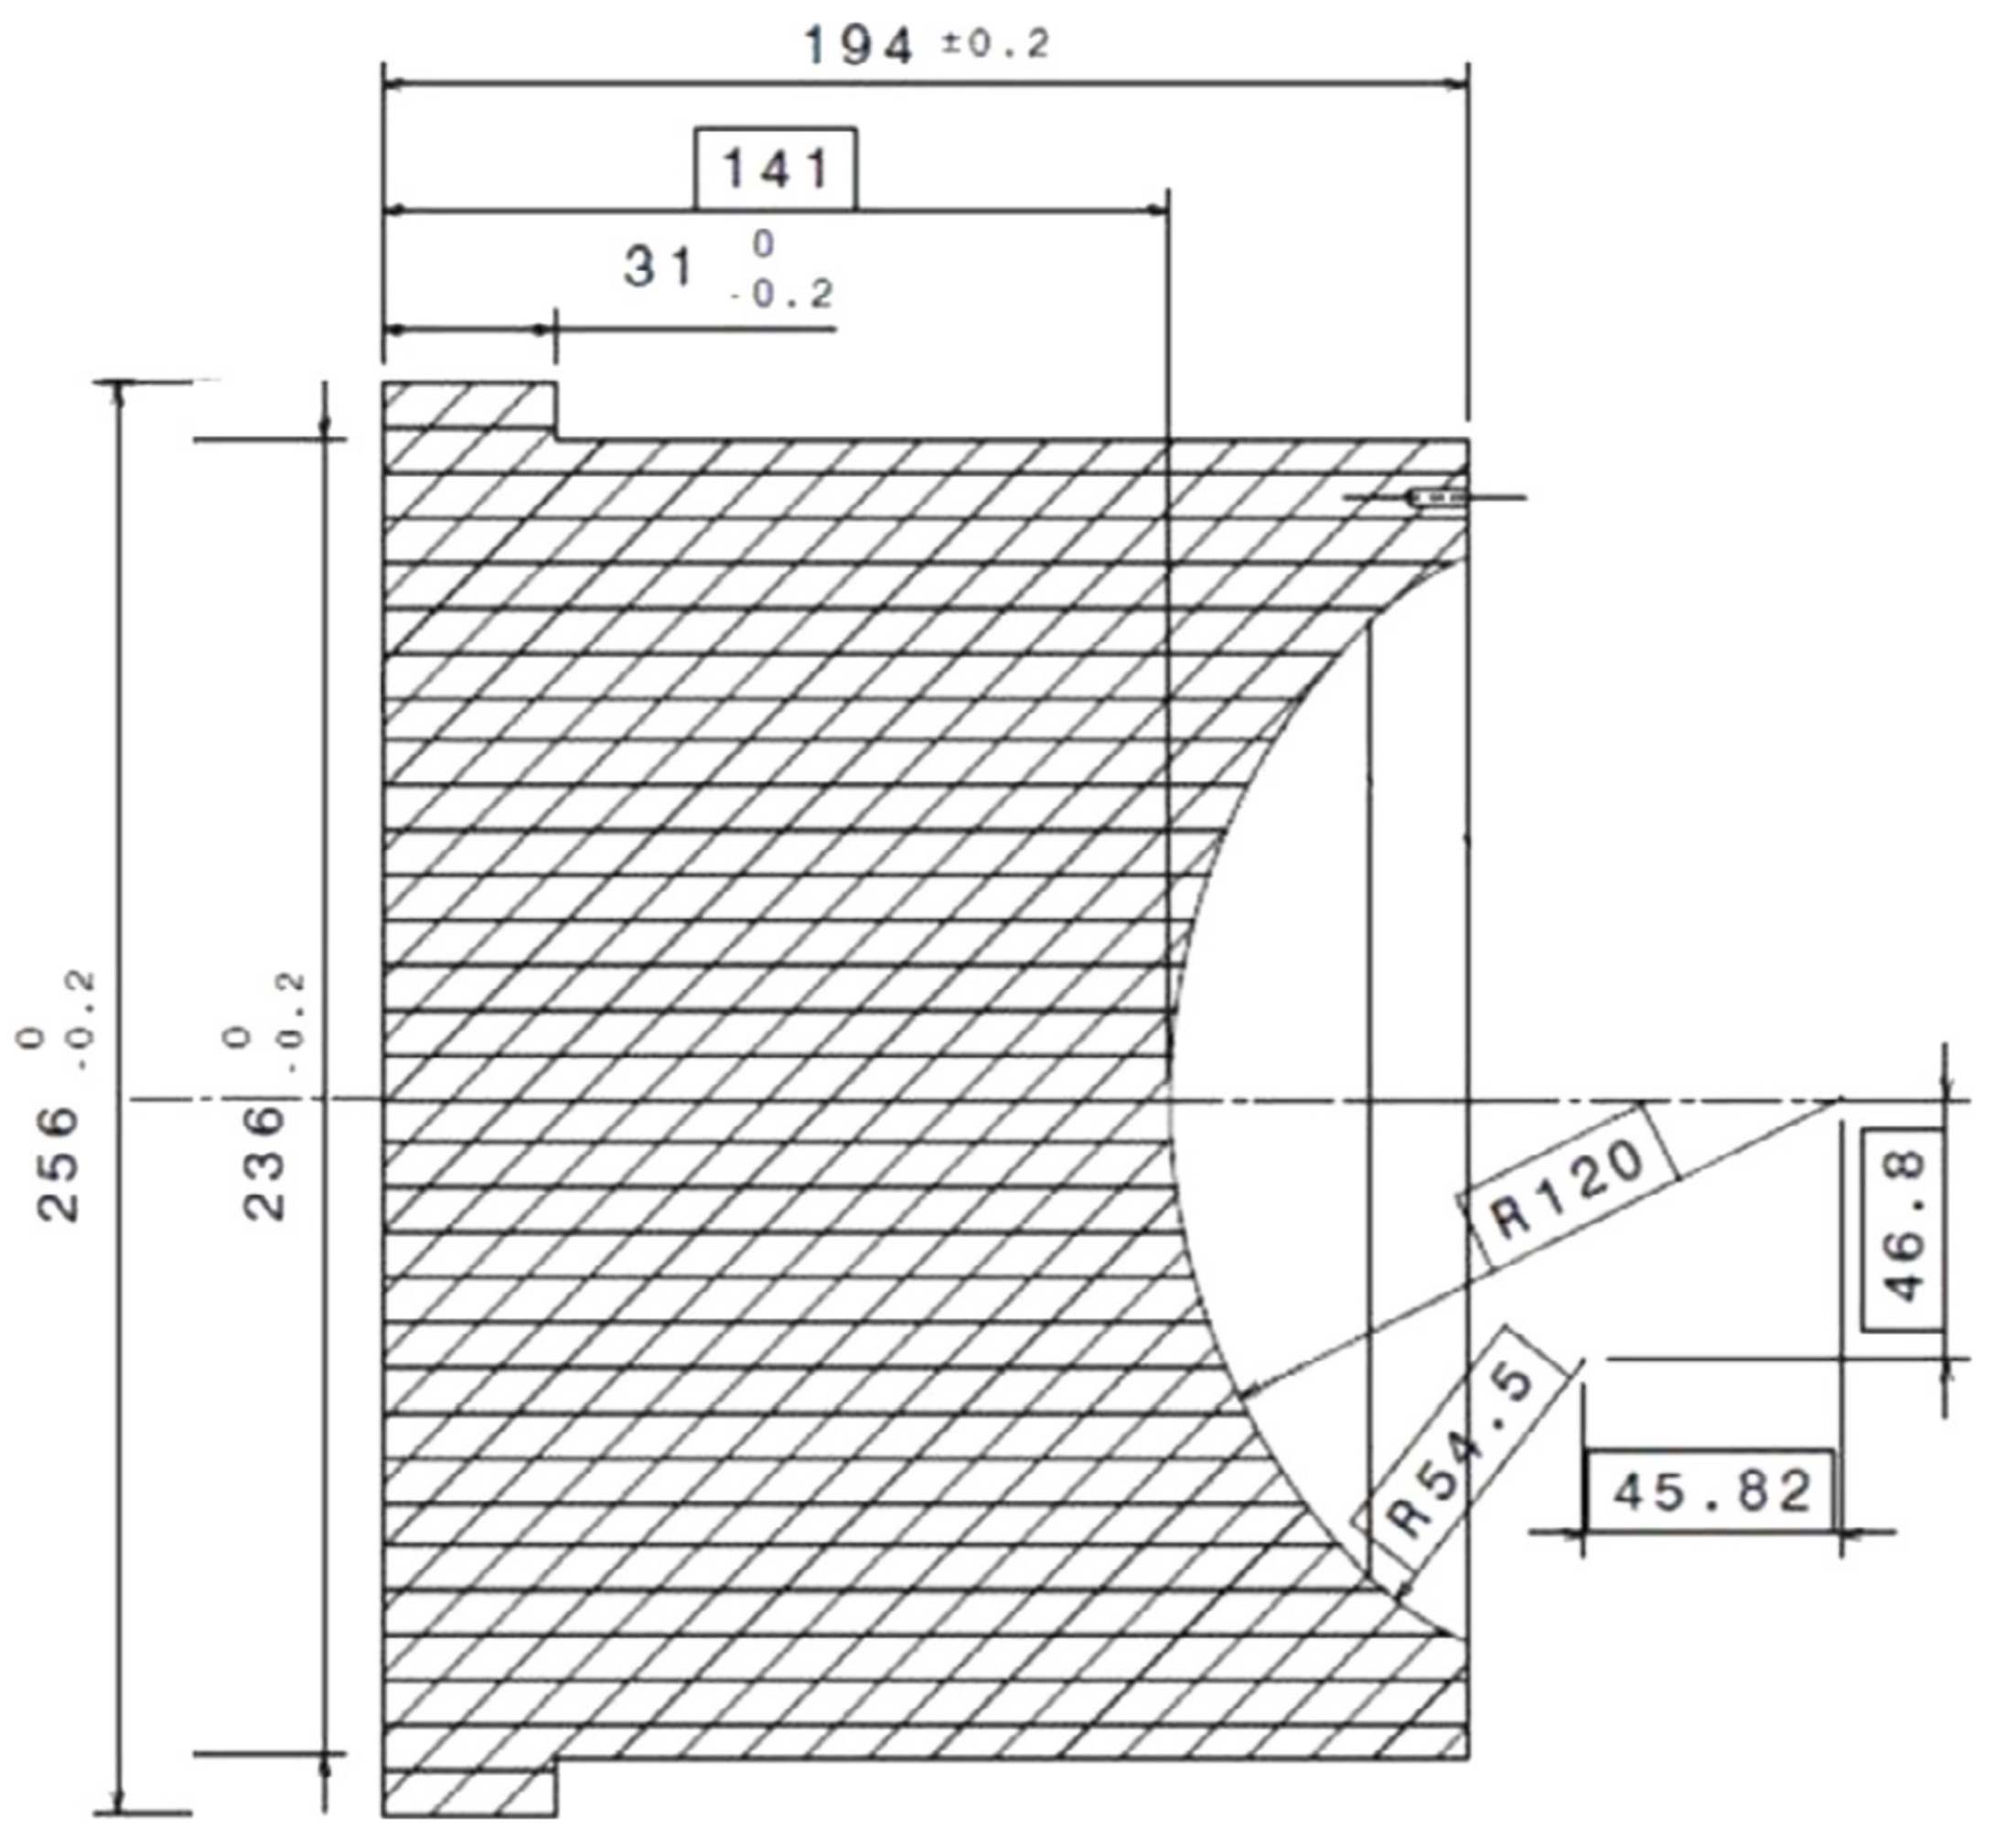
\includegraphics[height=0.95\textwidth]{SNdemonstrator/fig_SNdemonstrator/scintillator_plan.pdf}
  \end{subfigure}
  \hfill
  \begin{subfigure}[t]{0.49\textwidth}
    \centering
    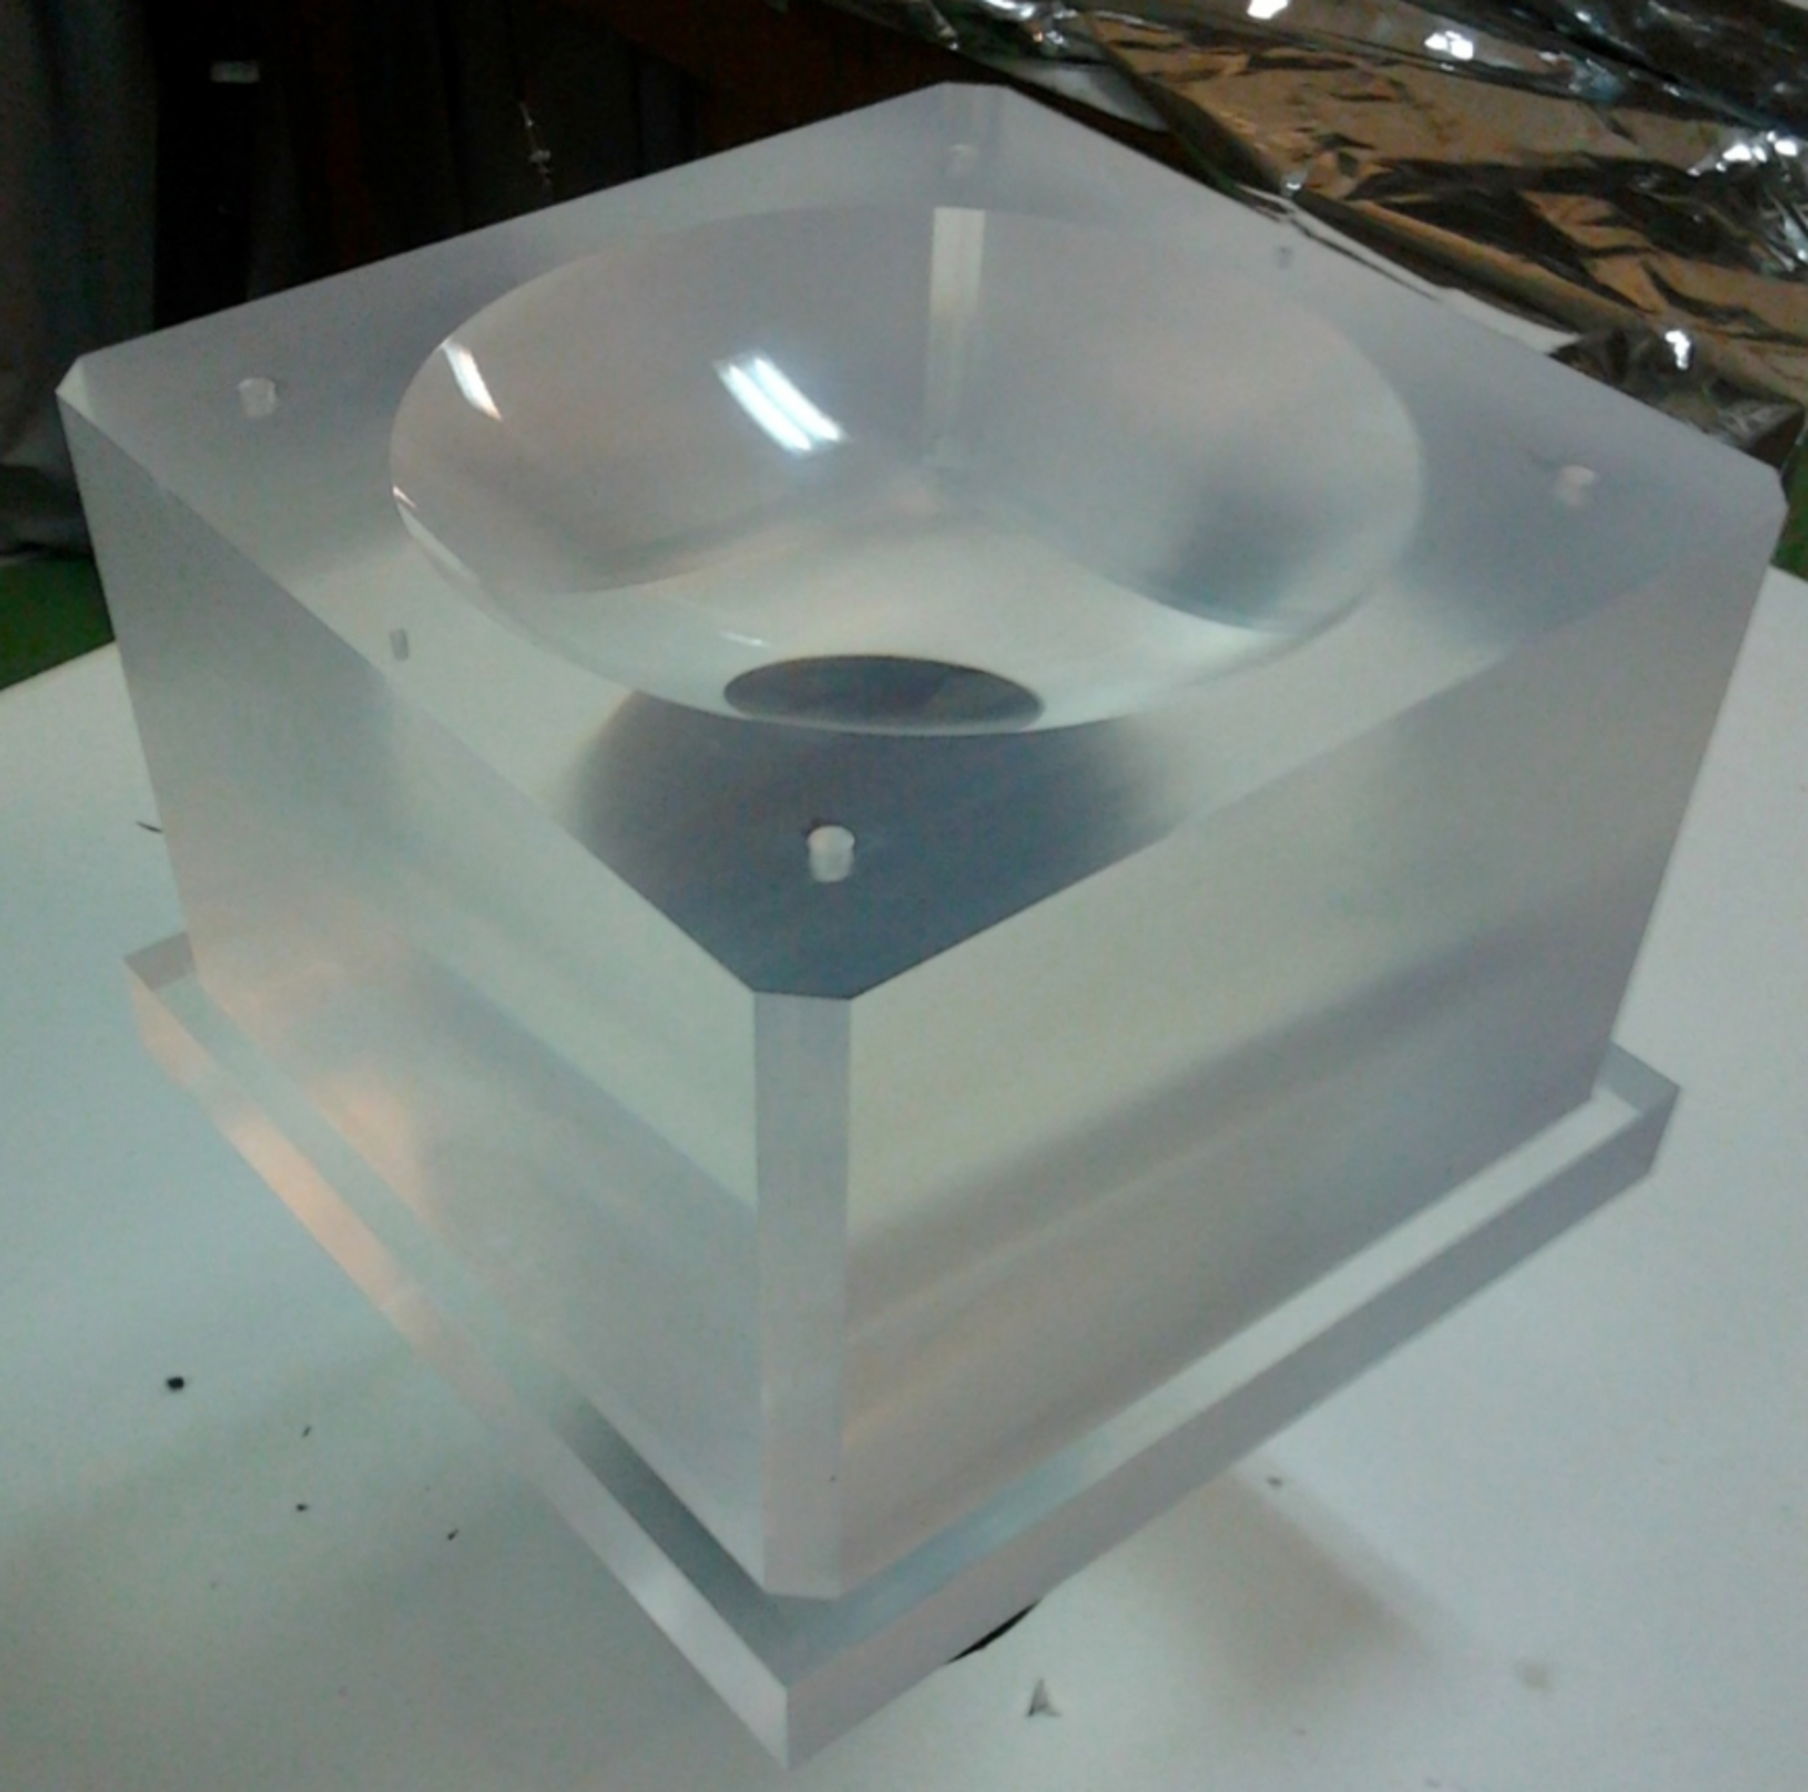
\includegraphics[height=0.95\textwidth]{SNdemonstrator/fig_SNdemonstrator/scintillator_pic.pdf}
  \end{subfigure}
  \caption{Geometry of a polystyrene cuboid scintillator block designed for the SuperNEMO demonstrator.
    The polystyrene is hollowed out to receive the photomultiplier bulb.
    \label{fig:scintillator_design}}
\end{figure}

The incoming particles (electrons, positrons or photons) enter the plastic scintillator and interact by ionisation.
The scintillator thus emits scintillation photons proportionally to the deposited energy, propagating through the scintillating medium.
Wave-length shifters ensure the light is not re-absorbed by the scintillator material.
Some of the scintillation photons are then collected by the photomultiplier photocathode.


\subsubsection*{Photomultipliers}

The SuperNEMO calorimeter requires a PM with a high quantum efficiency, a good photoelectron collection efficiency, a linear gain with energy, a high radiopurity, a good time resolution and low dark currents.
The PM used for the NEMO-$3$ experiment were mainly Hamamatsu $5$~inch types.
For the SuperNEMO demonstrator, $8$~inches PMs (R5912-MOD Hamamatsu) were chosen in order to match de designed scintillators.
They also allow to reduce the number of electronic channels, as well as to increase the photo-detection surface compared with its predecessor, to improve the energy measurement.

When reaching the photocathode, some of the scintillation photons are absorbed and photoelectrons are emitted through the photoelectric effect (Fig.~\ref{fig:PMT_design}).
These electrons drift to the first dynode under the influence of a high electric potential difference.
Electrons ionise this dynode when reaching it, amplifying the number of electrons which will in turn drift into the next dynode.
This drift/ionisation cascade amplifies the initial amount of charge collected by the last dynode, creating a measurable electric current.
The gain reached by $8$~inches SuperNEMO PMs is $10^{6}$.
\begin{figure}[h!]
\centering
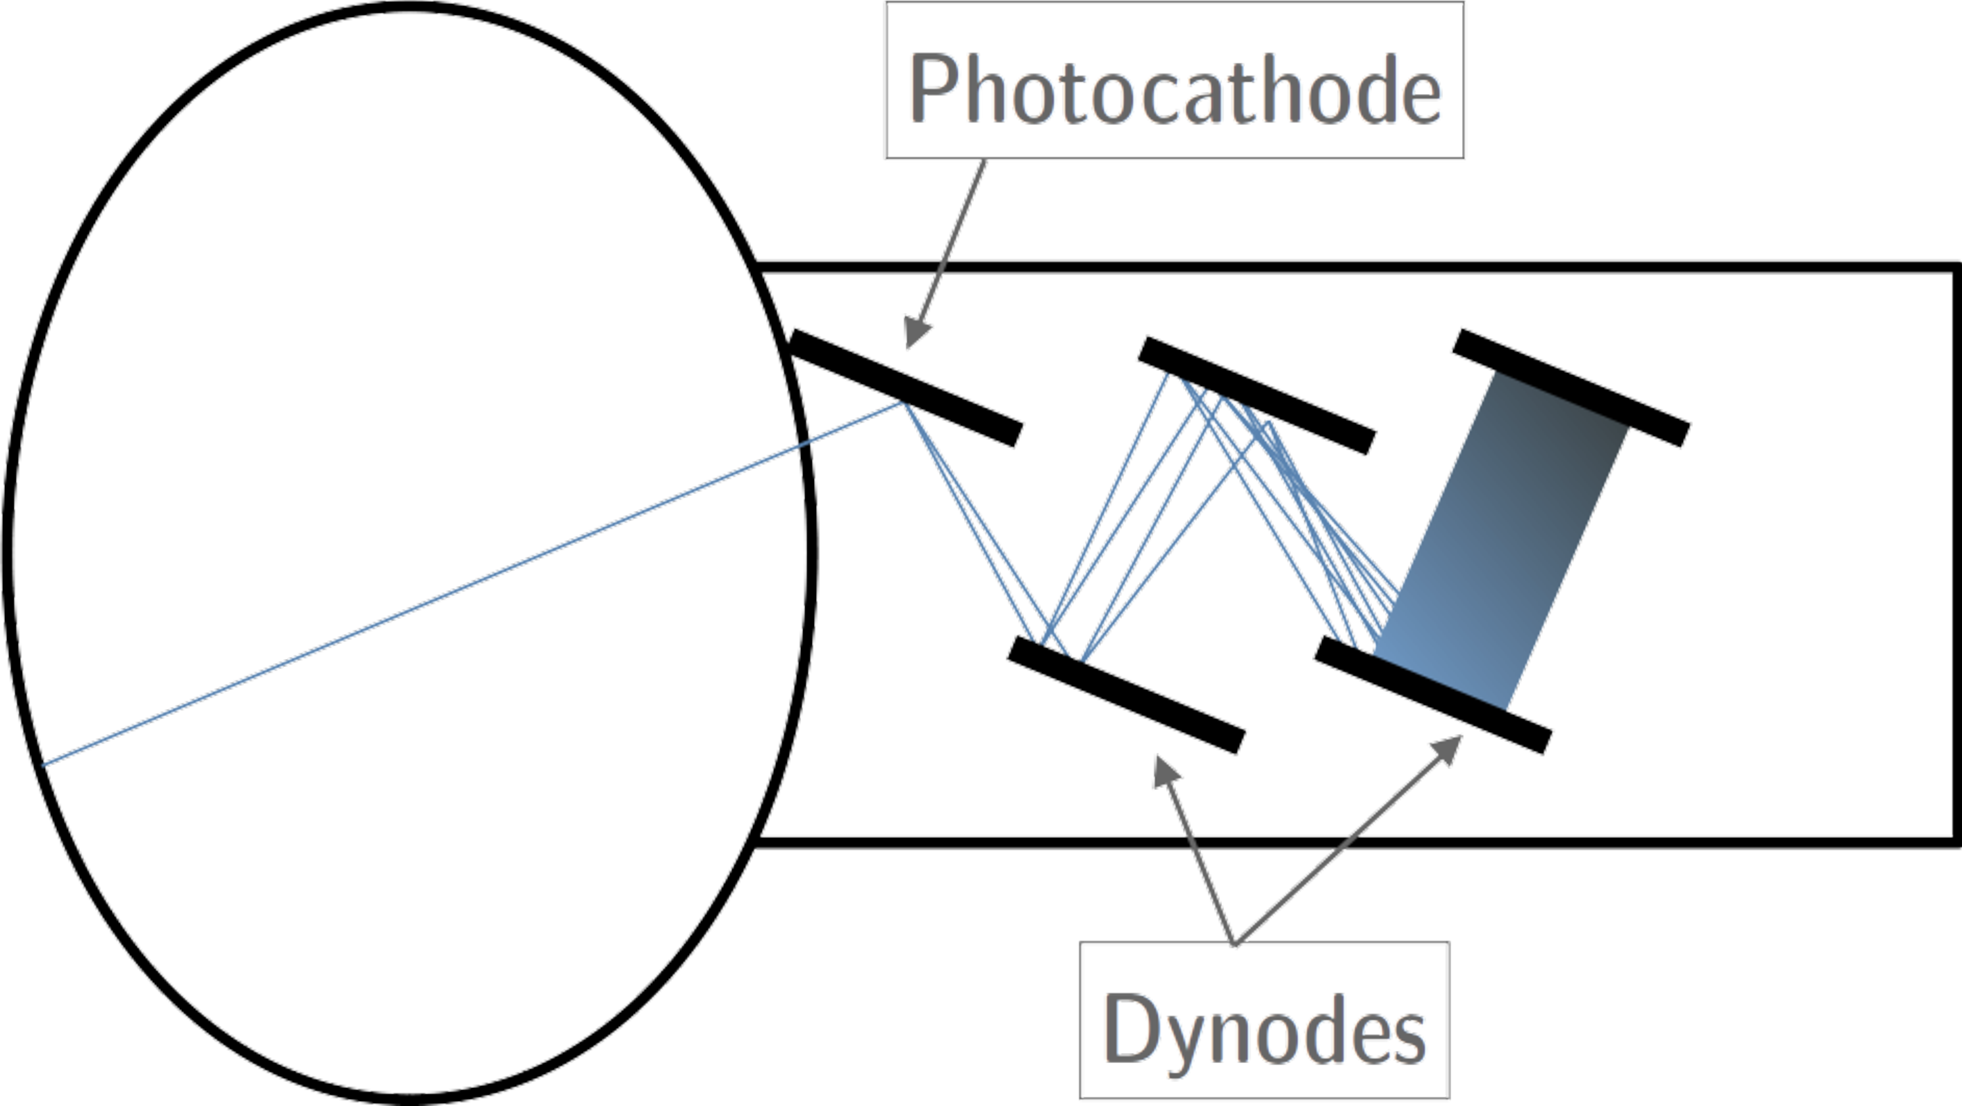
\includegraphics[width=0.7\textwidth]{SNdemonstrator/fig_SNdemonstrator/PMT_plan.pdf}
\caption{Basic operation principle of a photomultiplier.
  A scintillation photon enters the glass bulb of the PM and reaches the photocathode.
  The photoelectrons created through photoelectric effect are then multiplied by several dynodes under the influence of a high electric field.
\label{fig:PMT_design}}
\end{figure}

The quantum efficiency of the chosen photomultipliers were optimised for $400$~nm wave-lengths (that of the photons arriving on the photocathode) and is equal to $35$\% (compared to the $25$\% for NEMO-$3$).
The photoelectrons collection efficiency and linearity were also improved, increasing the number of photoelectrons to $\sim1000$ for $1$~MeV electrons in order to reach the $8$\% energy resolution at $1$~MeV.


\subsubsection*{Optical modules and mechanical design}

Scintillators and photomultipliers are assembled together by the CENBG team (Bordeaux) to constitute so-called \emph{optical modules} (Fig.~\ref{fig:scintillator_PMT}).
They are joined together using RTV615 glue.
A surface polishing and an optical gel with a refractive index comprised between the indices of the PM glass and the scintillator also helps the optical coupling.
Each optical module is protected by a magnetic shielding, whose usefulness is detailed in Sec.~\ref{subsec:magnetic_field}.
Groups of $8$ optical modules are pre-assembled for easy transport.
Finally, the calorimeter was assembled in its entirety at LSM during the summer $2016$ (Fig.~\ref{fig:calo_installation}).
\begin{figure}[h!]
\centering
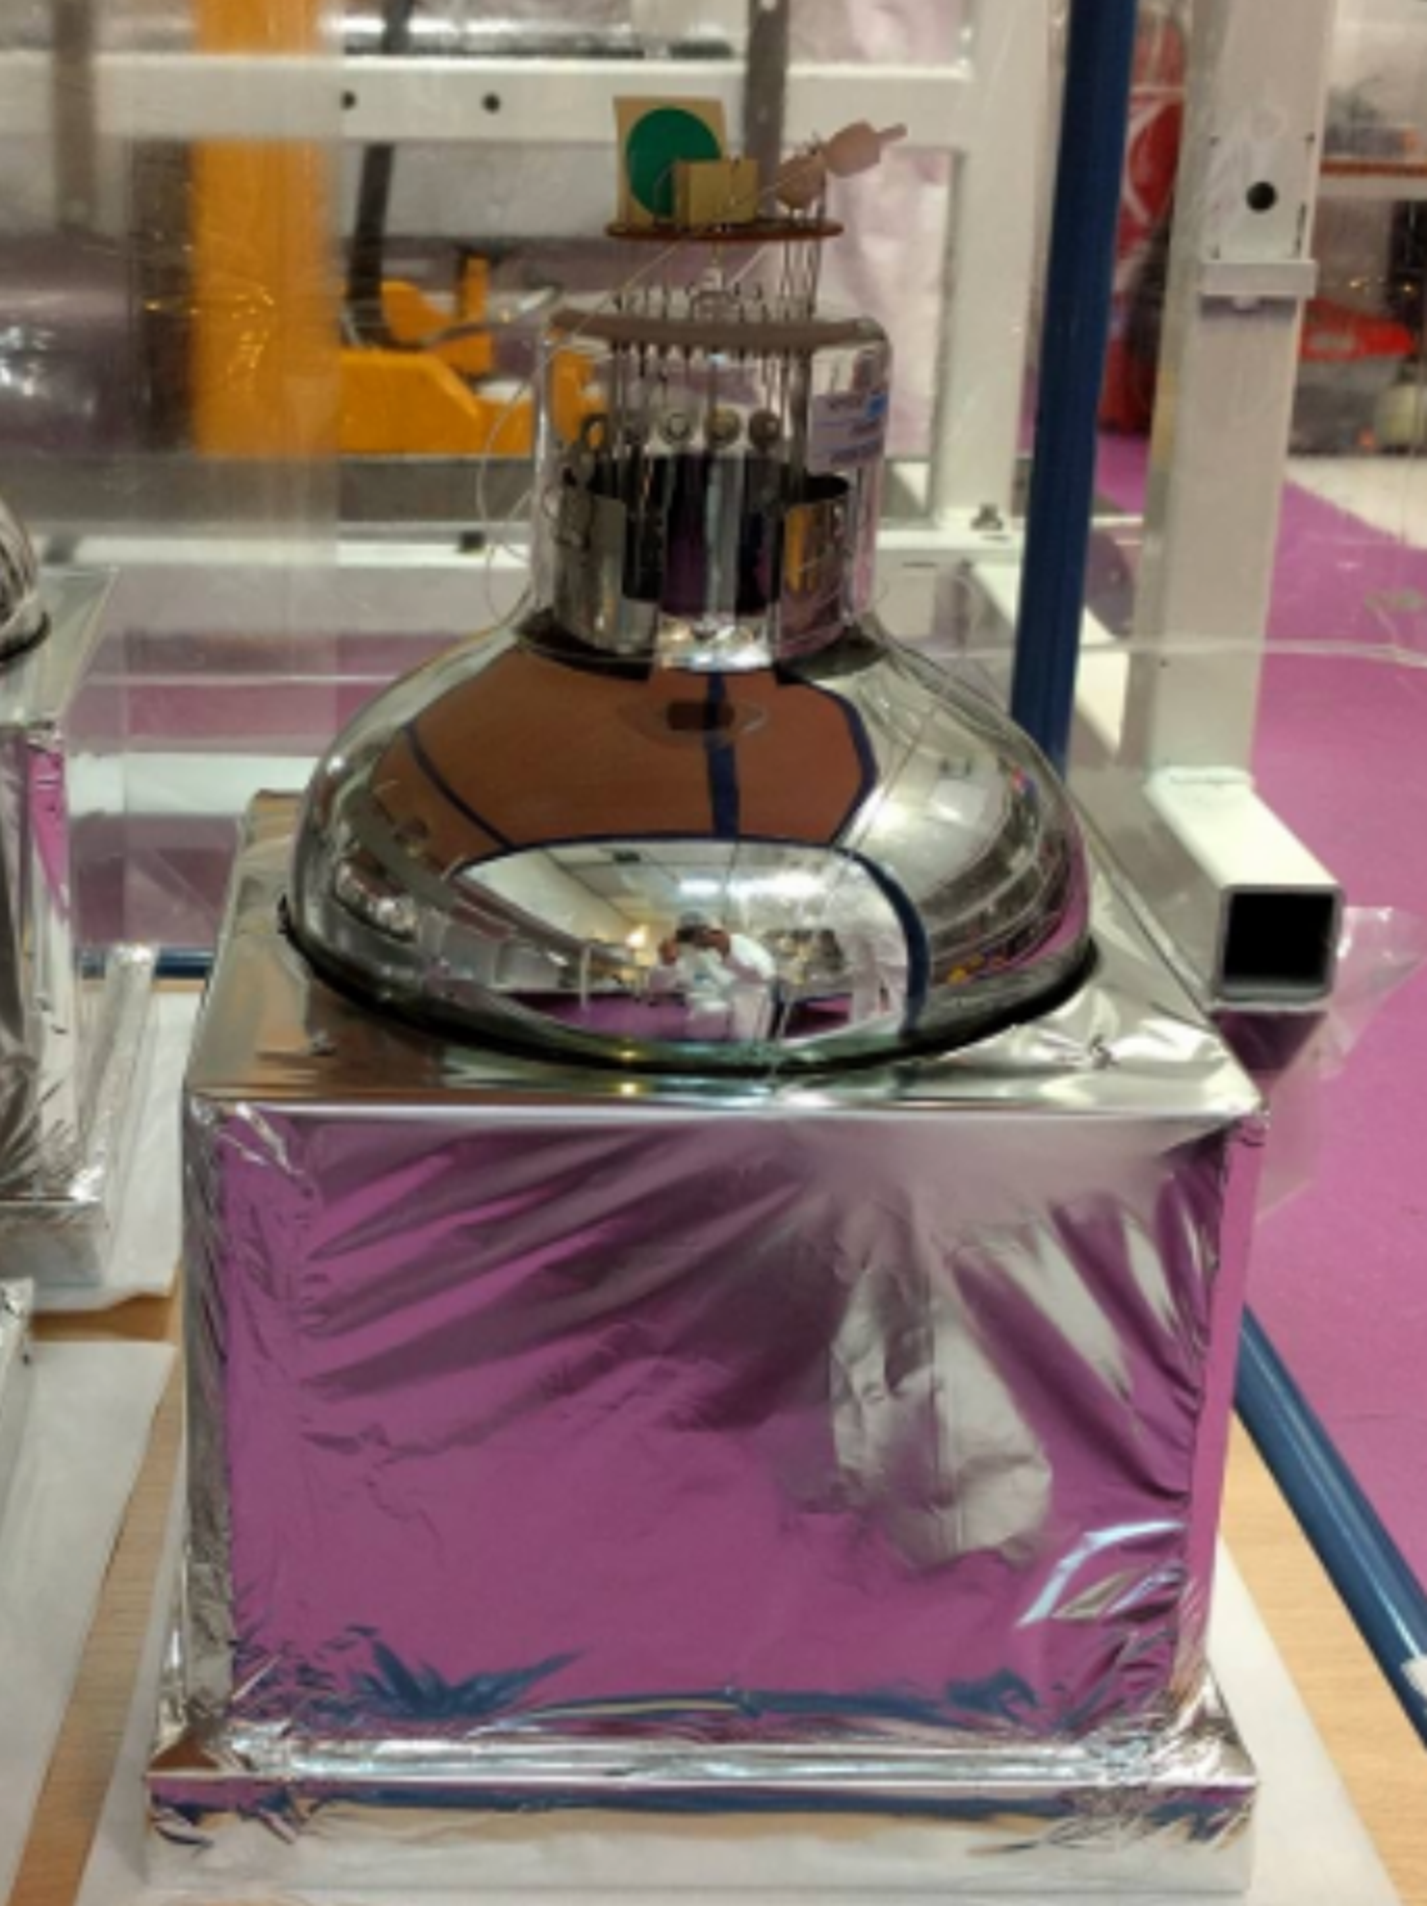
\includegraphics[width=0.4\textwidth]{SNdemonstrator/fig_SNdemonstrator/scintillator_wrap.pdf}
\caption{A scintillator coupled with a PM.
  The shiny wrapping around the scintillator is the aluminised Mylar.
\label{fig:scintillator_PMT}}
\end{figure}
\begin{figure}[!h]
\centering
\begin{subfigure}[t]{0.95\textwidth}
  \centering
  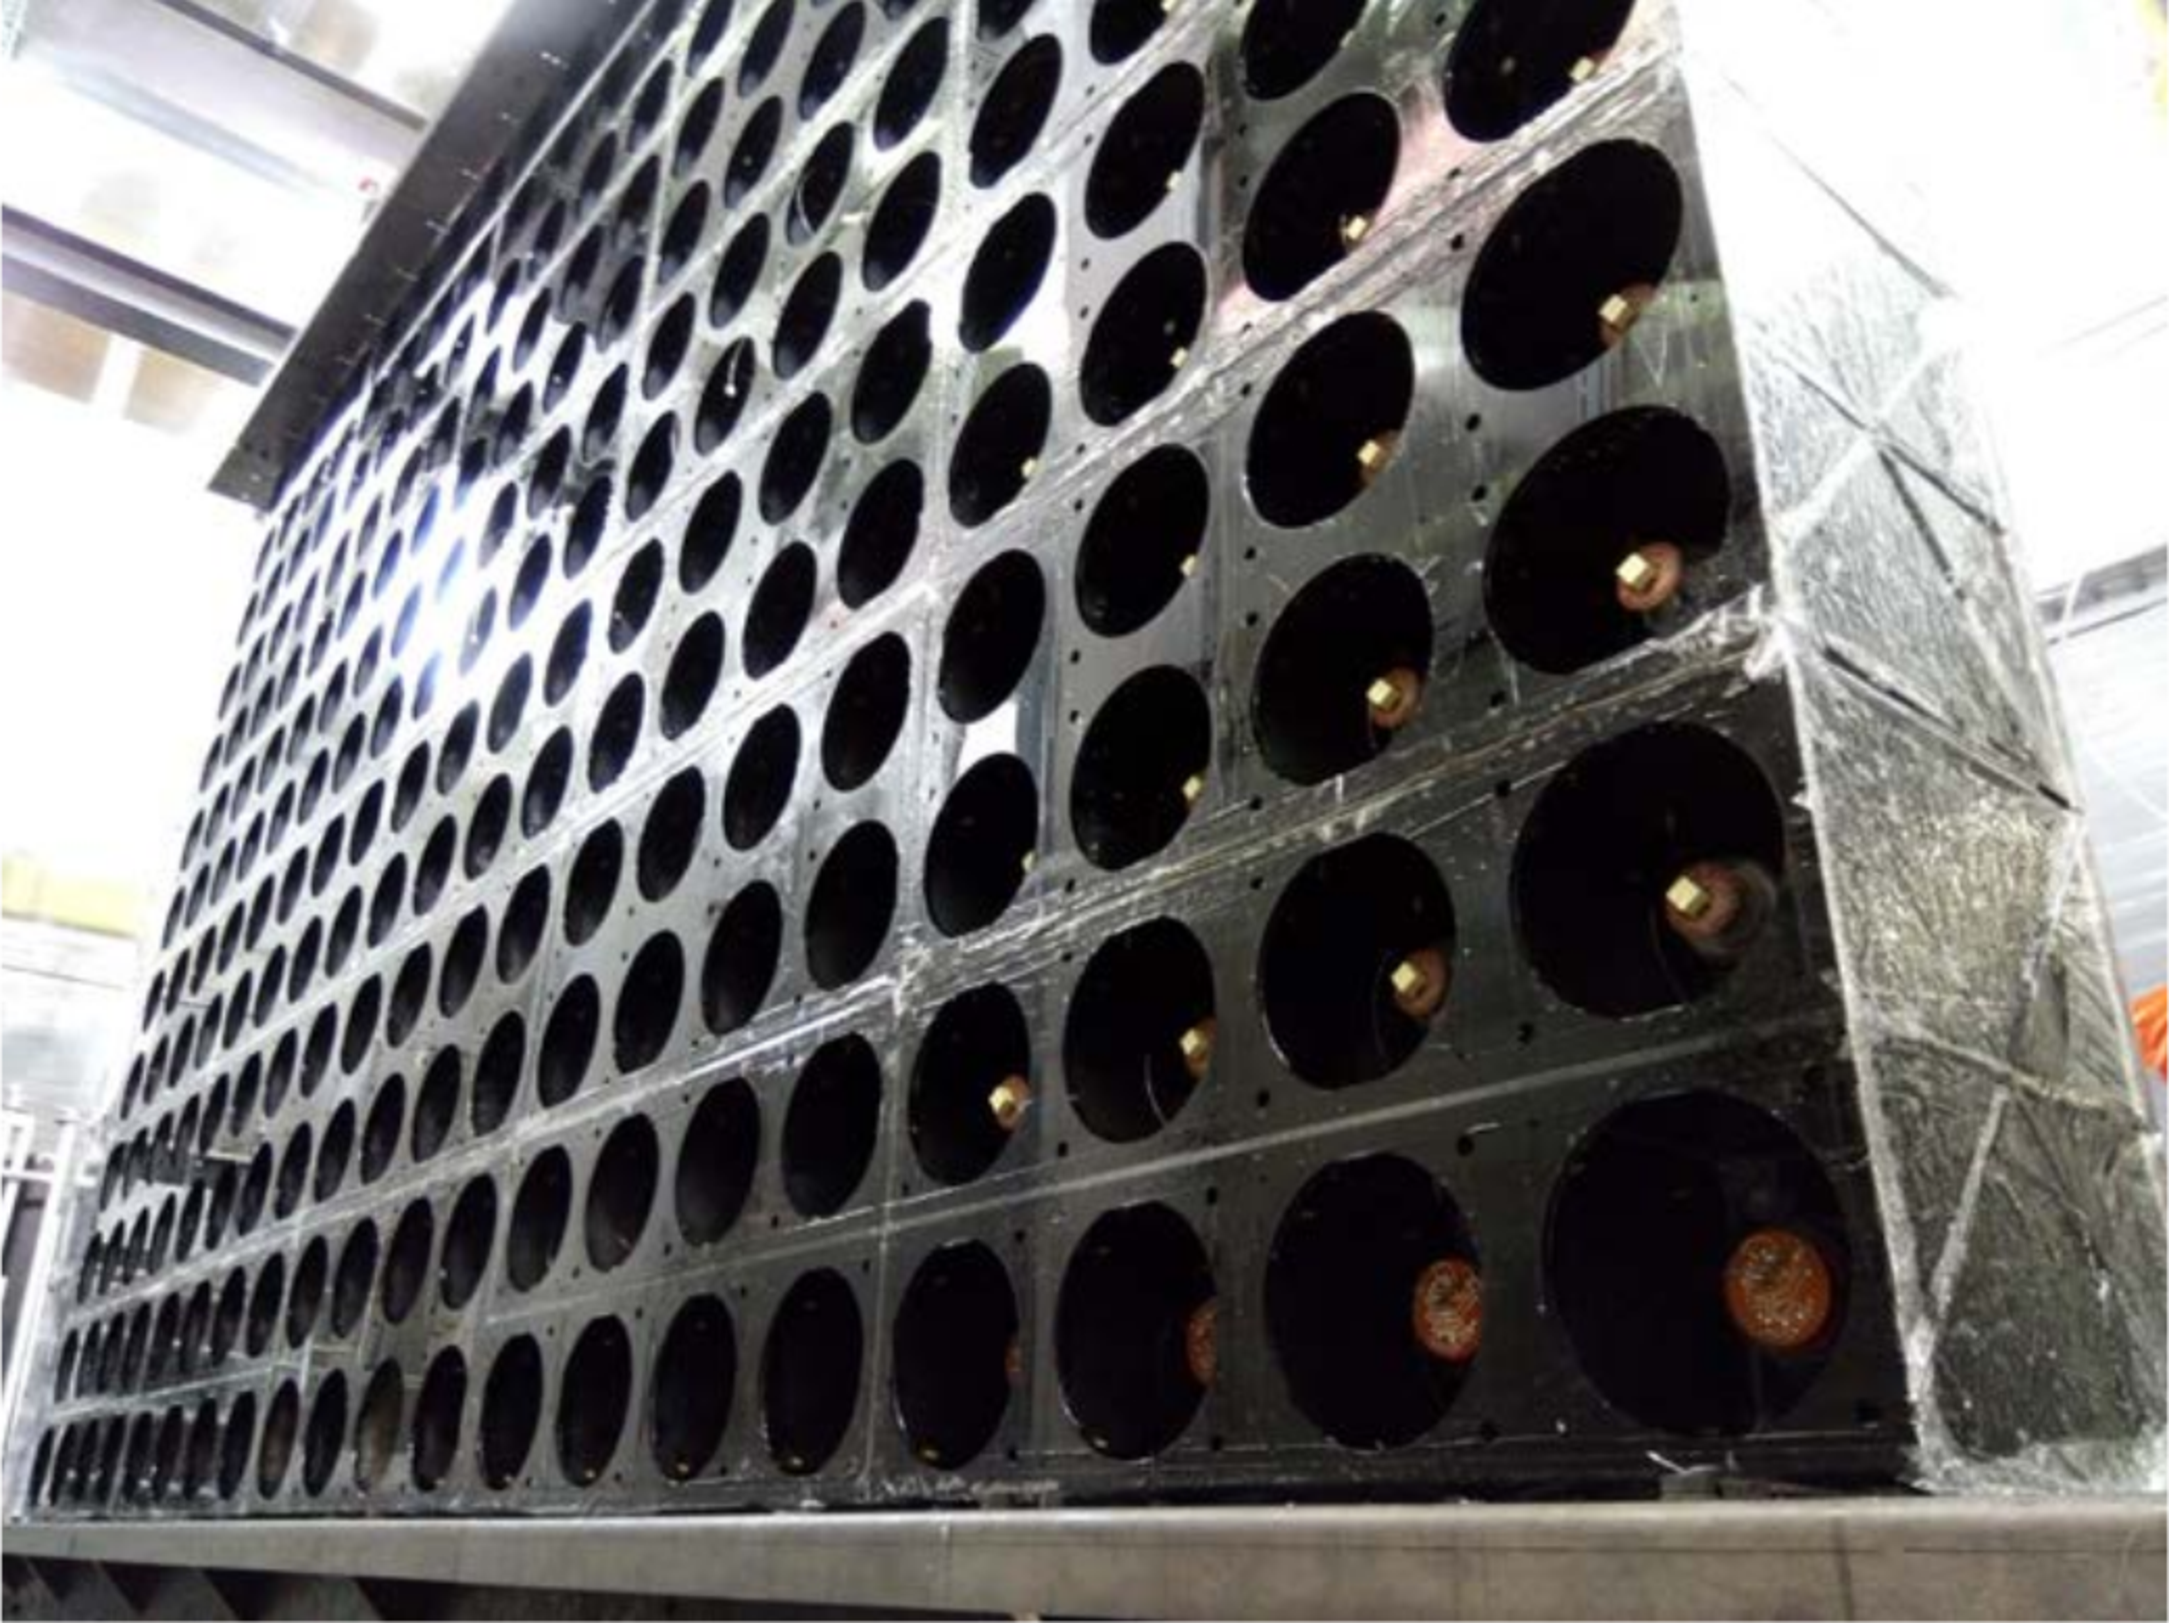
\includegraphics[width=0.9\textwidth]{SNdemonstrator/fig_SNdemonstrator/main_wall_back_view.pdf}
  \captionsetup{justification=justified}
  \caption{Back view of one calorimeter main wall.
    \label{subfig:cont_Pint_ROI}}
\end{subfigure}
\vskip\baselineskip
\begin{subfigure}[t]{0.95\textwidth}
  \centering
  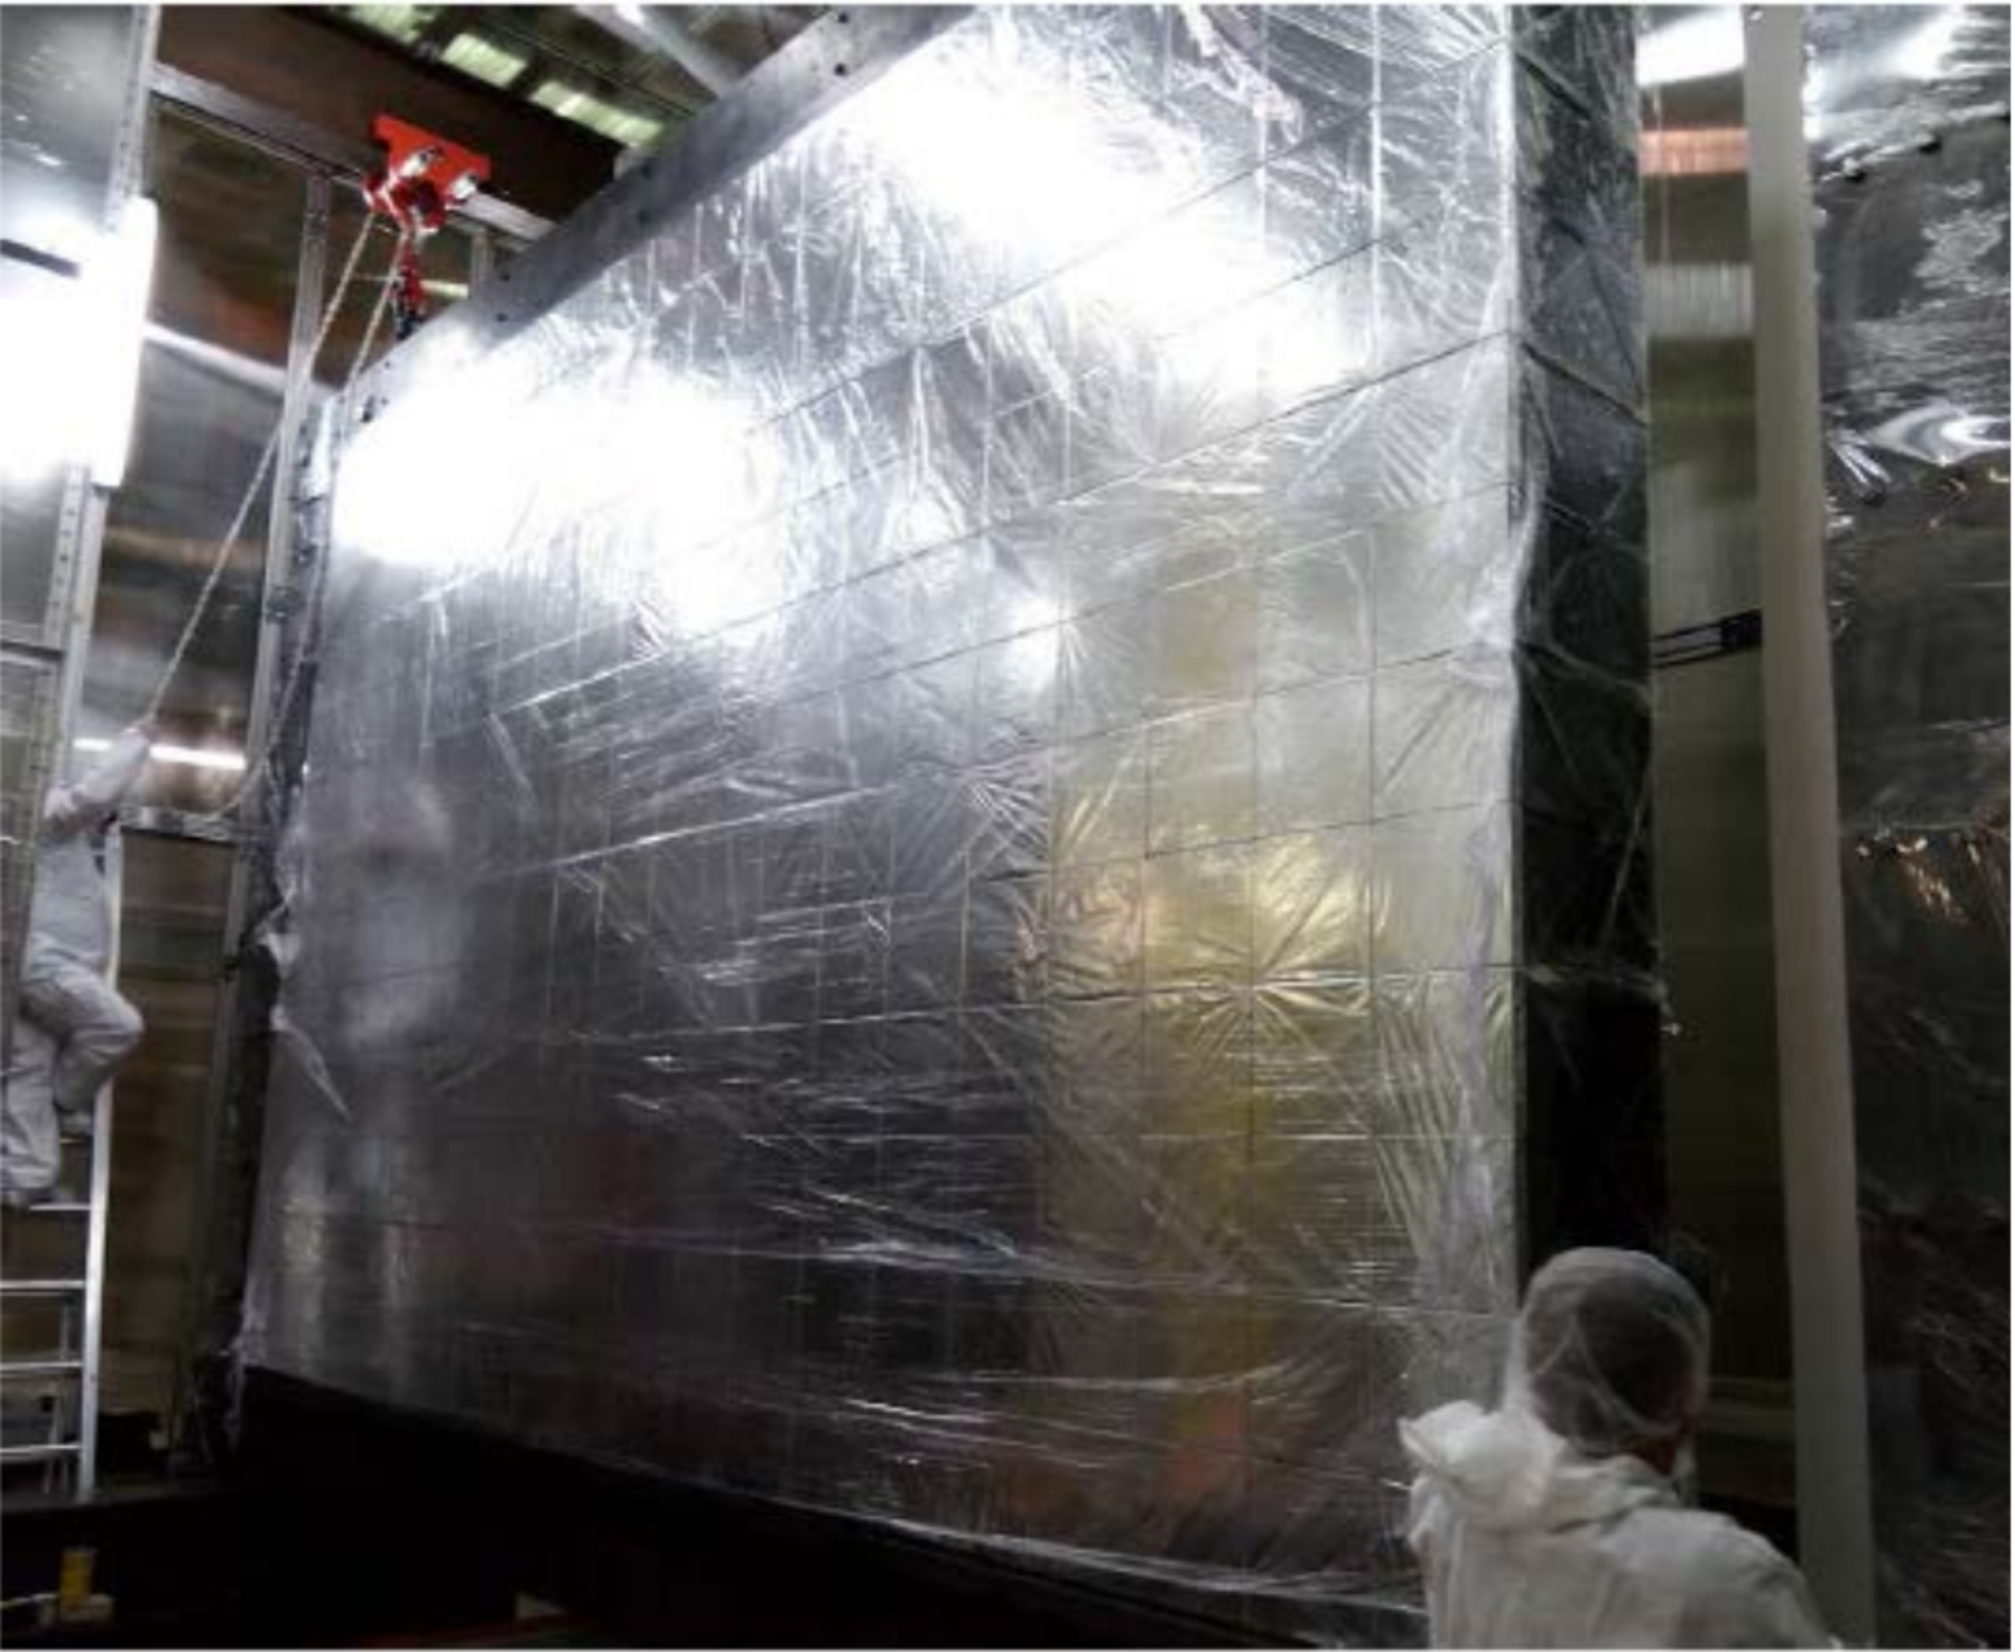
\includegraphics[width=0.9\textwidth]{SNdemonstrator/fig_SNdemonstrator/main_wall_front_view.pdf}
  \captionsetup{justification=justified}
  \caption{Front view of one calorimeter main wall.
    \label{subfig:}}
\end{subfigure}
\caption{Installation at LSM of one of the two main walls of the SuperNEMO calorimeter (summer $2016$).
  \label{fig:calo_installation}}
\end{figure}

The calorimeter of SuperNEMO is divided into three distinct sections.
\begin{itemize}
\item Two main calorimeter walls (one French side and one Italian side), parallel to the source foils, one on each side of the detector.
  Each wall is composed of $13\times20$ blocks, for a total of $520$ optical modules.
  The first and last optical module rows are built with $5$~inches PMs recovered from NEMO-$3$, while others are $8$~inches.
  NEMO-$3$ PMs have a worse resolution than $8$~inches but they will detect almost no electrons as these rows are mainly screened by the cathode rings in front of the scintillators.
  However, they insure a complete coverage for the detection of $\gamma$ particles.
\item Gamma-Veto optical modules are located at the top and bottom of the demonstrator: $2$ columns of $16$ on each side of the source, for a total of $64$.
  They are only used as a veto system against $\gamma$'s.
\item X-walls are located on each detector side: $2$ columns of $16$ are located on the mountain side, same on the tunnel side, for a total of $128$ optical modules.
  They are directly exposed to the tracker volume.
\end{itemize}
The optical modules constituting the X-walls and Gamma-Vetos are directly fixed on the tracker frame.
As they are composed of $5$~inches PMs, their energy resolution is more modest than the rest of the calorimeter ($12$\% FWHM at $1$~MeV for the X-wall blocks and $15$\% FWHM at $1$~MeV for the veto blocks).
Nevertheless, they ensure a $4\pi$ calorimetric coverage for $\gamma$ particles.

The commissioning of the SuperNEMO calorimeter started in $2018$ and is almost fully achieved (a scientific paper is currently being prepared).
During my PhD, I actively participated in this crucial phase for the detector development.


\subsection{The magnetic coil and the shieldings}
\label{subsec:magnetic_field}

After a neutron capture outside the detector, high energy gammas can be created and can cross the detector volume.
Electron/positron pair creation can then occur in the source, the two emitted particles sharing the energy of the initial photon.
If an electron/positron discrimination is impossible, this category of event can be harmful for the search for the $\zeronu$ decay.
For that reason, in the manner of NEMO-$3$, the SuperNEMO demonstrator will be equipped with a copper coil that will deliver a vertical (parallel to the wires) magnetic field inside the tracker chamber, in order to bend the charged particle trajectories.

\subsubsection*{The SuperNEMO magnetic field}

A three-dimensional representation of the SuperNEMO demonstrator is given in Fig.~\ref{fig:coil_3D} with the coil circled in red.
A study led by the collaboration allowed to determine that the optimal intensity for the magnetic field would be $25$~Gauss, allowing to bend the few MeV particle trajectories, thus providing a useful discrimination between electrons and positrons.
\begin{figure}[h!]
\centering
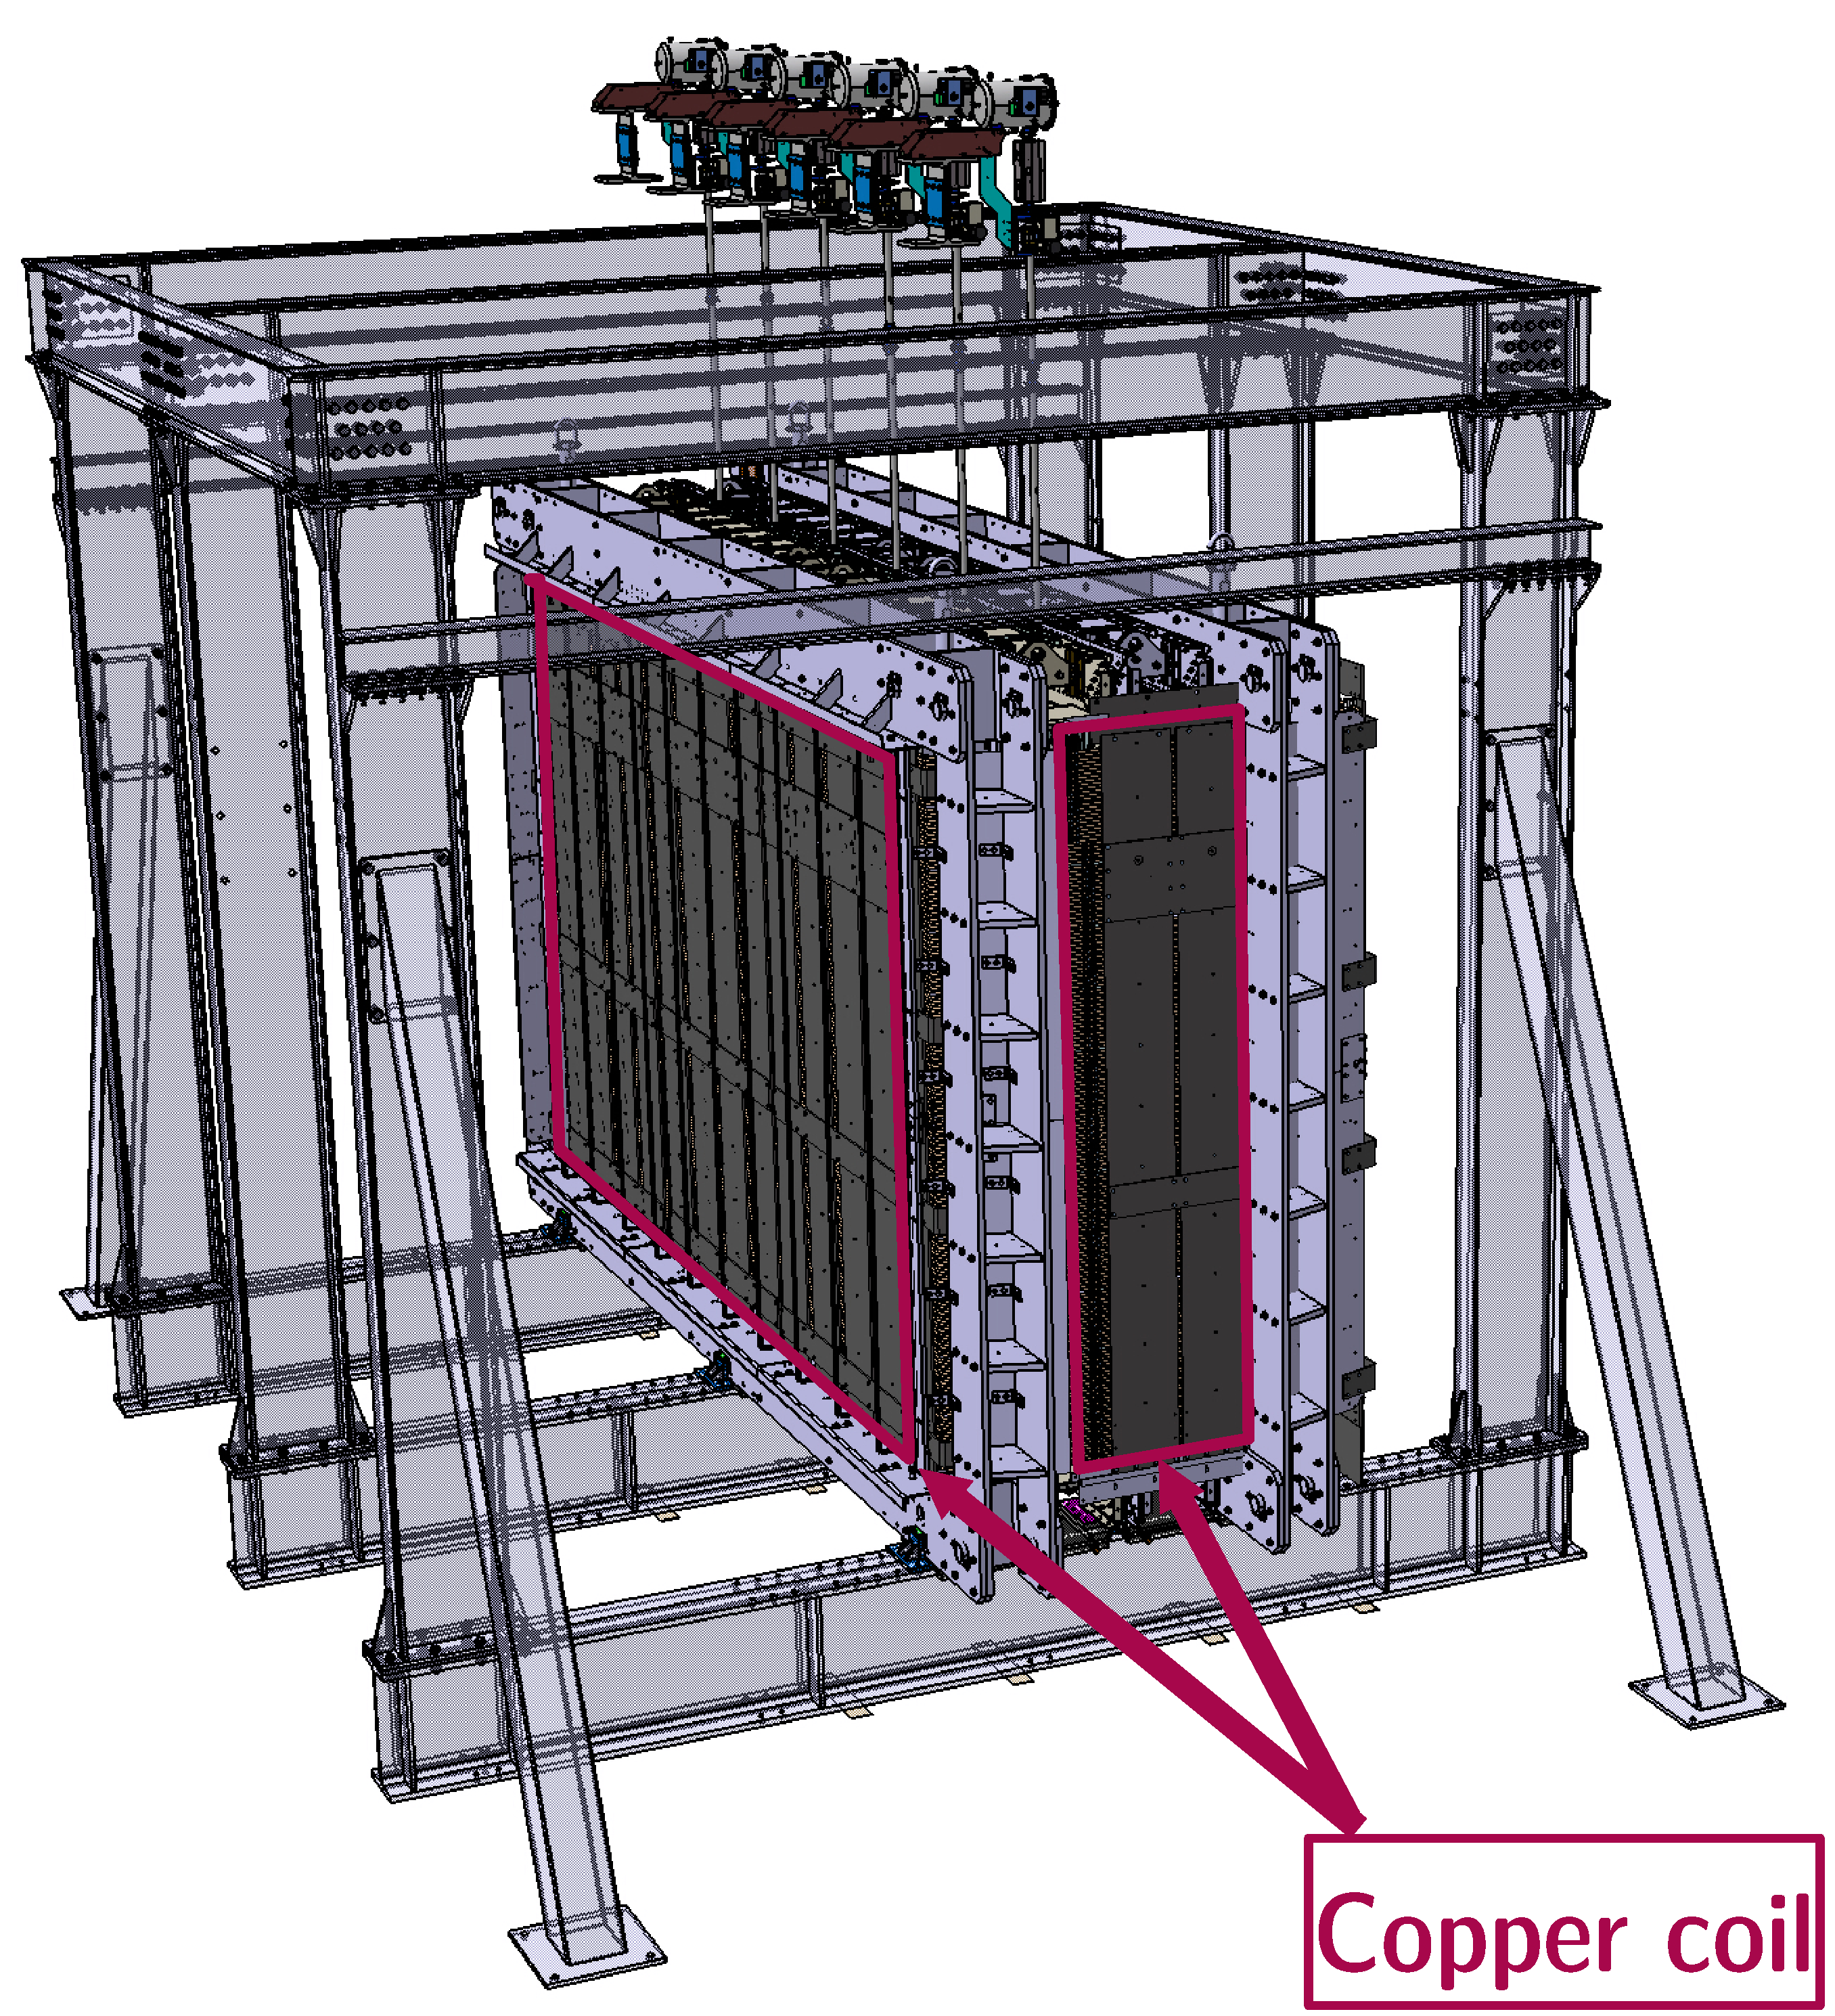
\includegraphics[height=0.8\textwidth]{SNdemonstrator/fig_SNdemonstrator/coil_3D.pdf}
\caption{3D representation of the SuperNEMO demonstrator, without the external iron shielding.
  The copper coil is circled in red.
\label{fig:coil_3D}}
\end{figure}


The copper coil is constituted of copper rods recycled from NEMO-$3$ and reshaped by the mechanics team at LAL to surround the demonstrator (Fig.~\ref{fig:coil_LAL}).
The coil is made of $200$ turns with $16$~mm steps, which makes it possible to generate the desired magnetic field while limiting the amount of heat produced.
The overall dimensions are $6097\times2198\times3483$~mm$^{3}$ and are supported by iron plates, for a total weight of $9$~tons.
The copper coil was planned to be installed by March $2020$ but was delayed due to the world health situation.
\begin{figure}[h!]
\centering
\includegraphics[height=0.5\textwidth]{SNdemonstrator/fig_SNdemonstrator/coil_lal.jpg}
\caption{One of the coil panel, recycled from NEMO-$3$.
\label{fig:coil_LAL}}
\end{figure}

\subsubsection*{Magnetic shieldings}

Unfortunately, the PMs are highly sensitive to the presence of a magnetic field inside the detector and their performances could be greatly impacted~\cite{CalvezThesis,internal:magnetic_field}.
Indeed, even a magnetic field as low as $1$~Gauss can prevent the low energy photoelectrons from reaching the first dynode and thus impact the PM energy resolution.
Therefore, $3$~mm thick pure iron shieldings have been designed to surround the optical modules and protect them from the magnetic field (Fig.~\ref{fig:magnetic_shields}).
The magnetic shieldings are separated by $10$~mm acrylic spacers (PMMA).
As done for NEMO-$3$, better shieldings would have been achieved with mu-metal, but this material is much more expensive and unfortunately less radio-pure.
Some of these mu-metal shields have however been recovered to protect the few $5$-inch PMs from X-wall and Gamma-Vetos which contribute less to the total radioactive isotope budget.
\begin{figure}[h!]
\centering
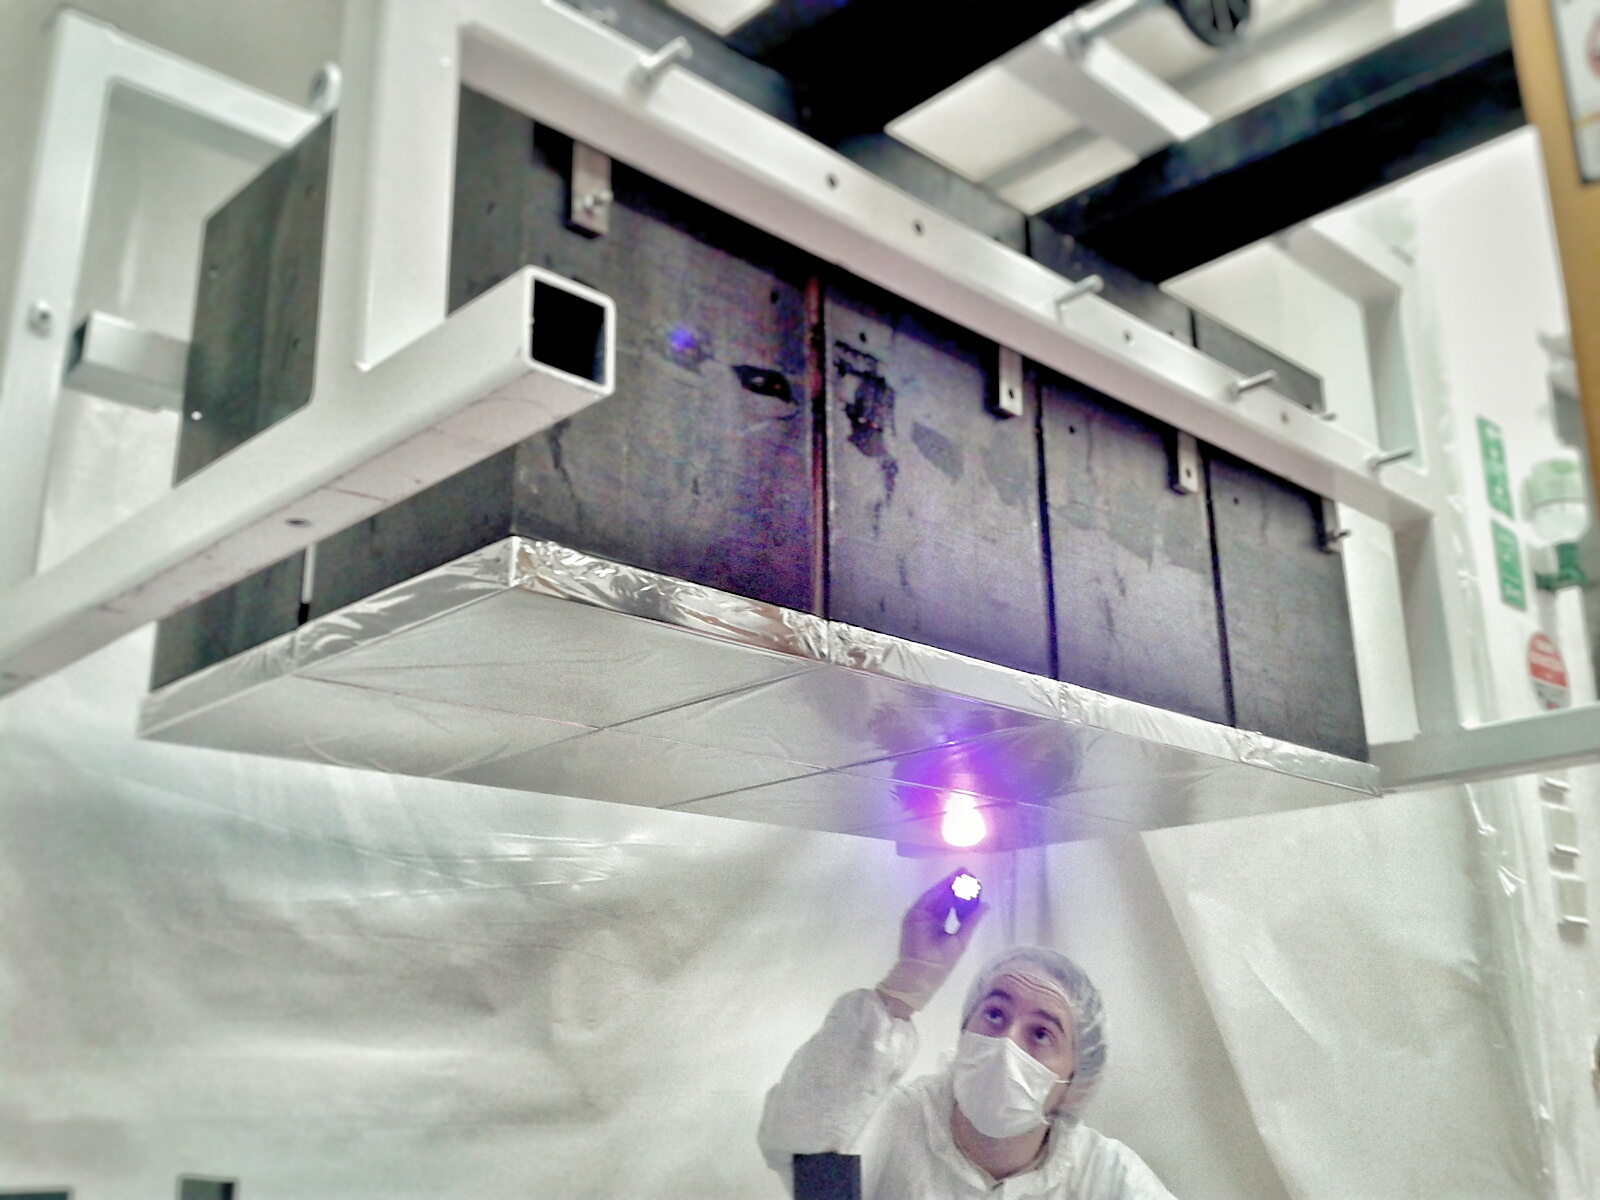
\includegraphics[height=0.5\textwidth]{SNdemonstrator/fig_SNdemonstrator/magnetic_shields.jpg}
\caption{A block of $8$ optical modules grouped together for installation at LSM.
  The magnetic shields are the black boxes surrounding the optical modules.
\label{fig:magnetic_shields}}
\end{figure}


\subsection{Calibration strategy}
\label{subsec:calib}

The SuperNEMO demonstrator is designed to have a long exposure time.
In this context, calibration systems are necessary to control regularly and calibrate the response of the detector.


\subsubsection*{Source deployment system}

The $^{207}$Bi isotope decays almost exclusively through electron capture to excited states of $^{207}$Pb.
The decay is followed by $^{207}$Pb de-excitation with $\gamma$-ray emission (the decay scheme is given in Fig.~\ref{fig:207Bi_decay_scheme}).
The $\gamma$-ray can convert in K,L or M electrons with a given probability through the internal conversion process, which is described in detail in Chapter~\ref{ch:timediff}.
The three corresponding electron energies are $976$~keV ($7.1$\% probability), $1050$~keV ($1.8$\% probability) and $1060$~keV ($0.4$\% probability).
\begin{figure}[h!]
\centering
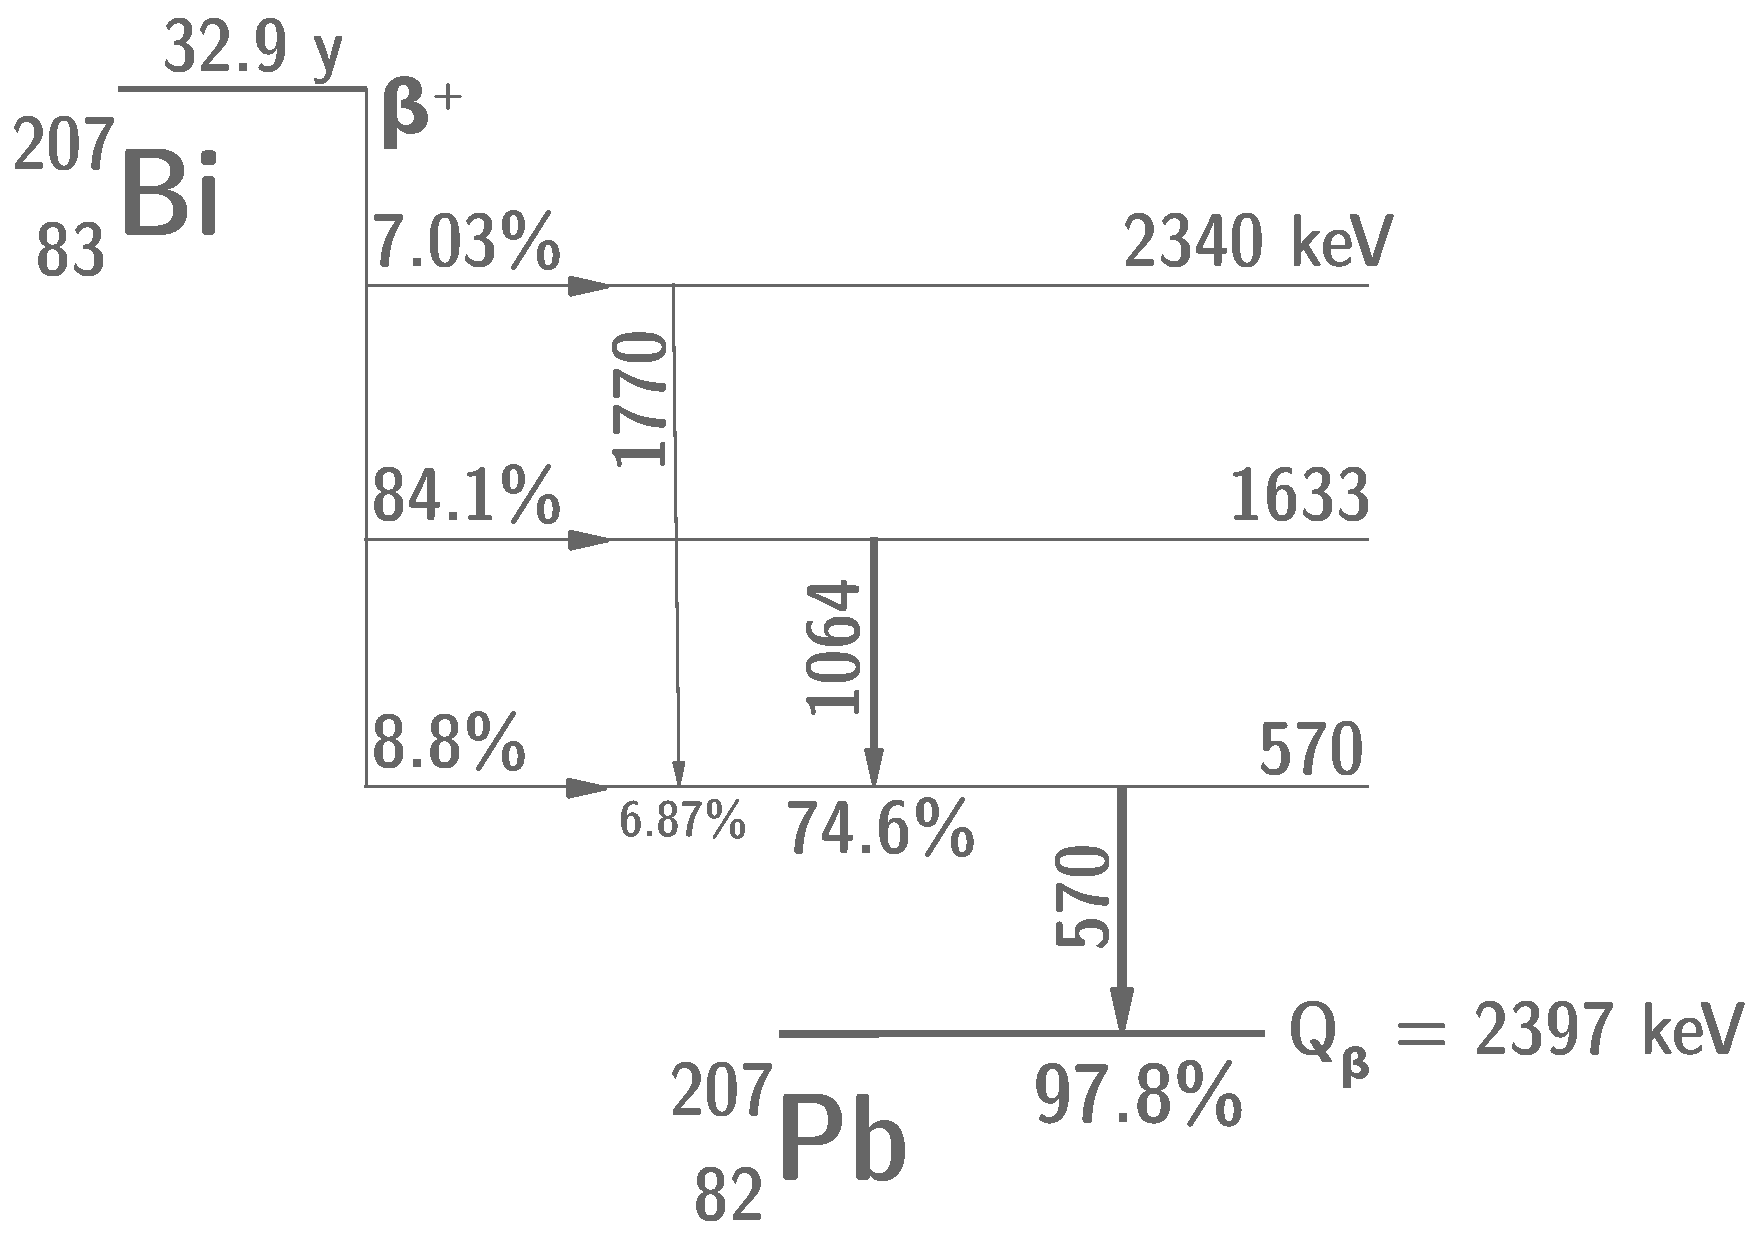
\includegraphics[height=0.5\textwidth]{SNdemonstrator/fig_SNdemonstrator/207Bi_decay_scheme.pdf}
\caption{Simplified decay scheme of the $^{207}$Bi isotope.
\label{fig:207Bi_decay_scheme}}
\end{figure}

$^{207}$Bi sources are used for SuperNEMO absolute energy calibrations: the three different electron energy peaks can be measured helping to follow and thus correct the response of the calorimeter modules with time.
In total $42$ sources ($7$ columns and $6$ rows) of around $130$~Bq are integrated to the so-called \emph{deployment system}, which is in charge of the automatic deployment of the calibration sources between the source foils (Fig.~\ref{fig:bi_sources}).
To do so, the Bismuth sources are attached at seven fixed points of six different stainless steal wires.
Each wire is wrapped around a wheel on top of the detector which may be rotated by a stepper motor, making it possible to introduce the sources into the detector source frame.
Daily runs are being considered to monitor the optical module gains with the conversion electrons.
\begin{figure}[!h]
  \centering
  \begin{subfigure}[t]{0.49\textwidth}
    \centering
    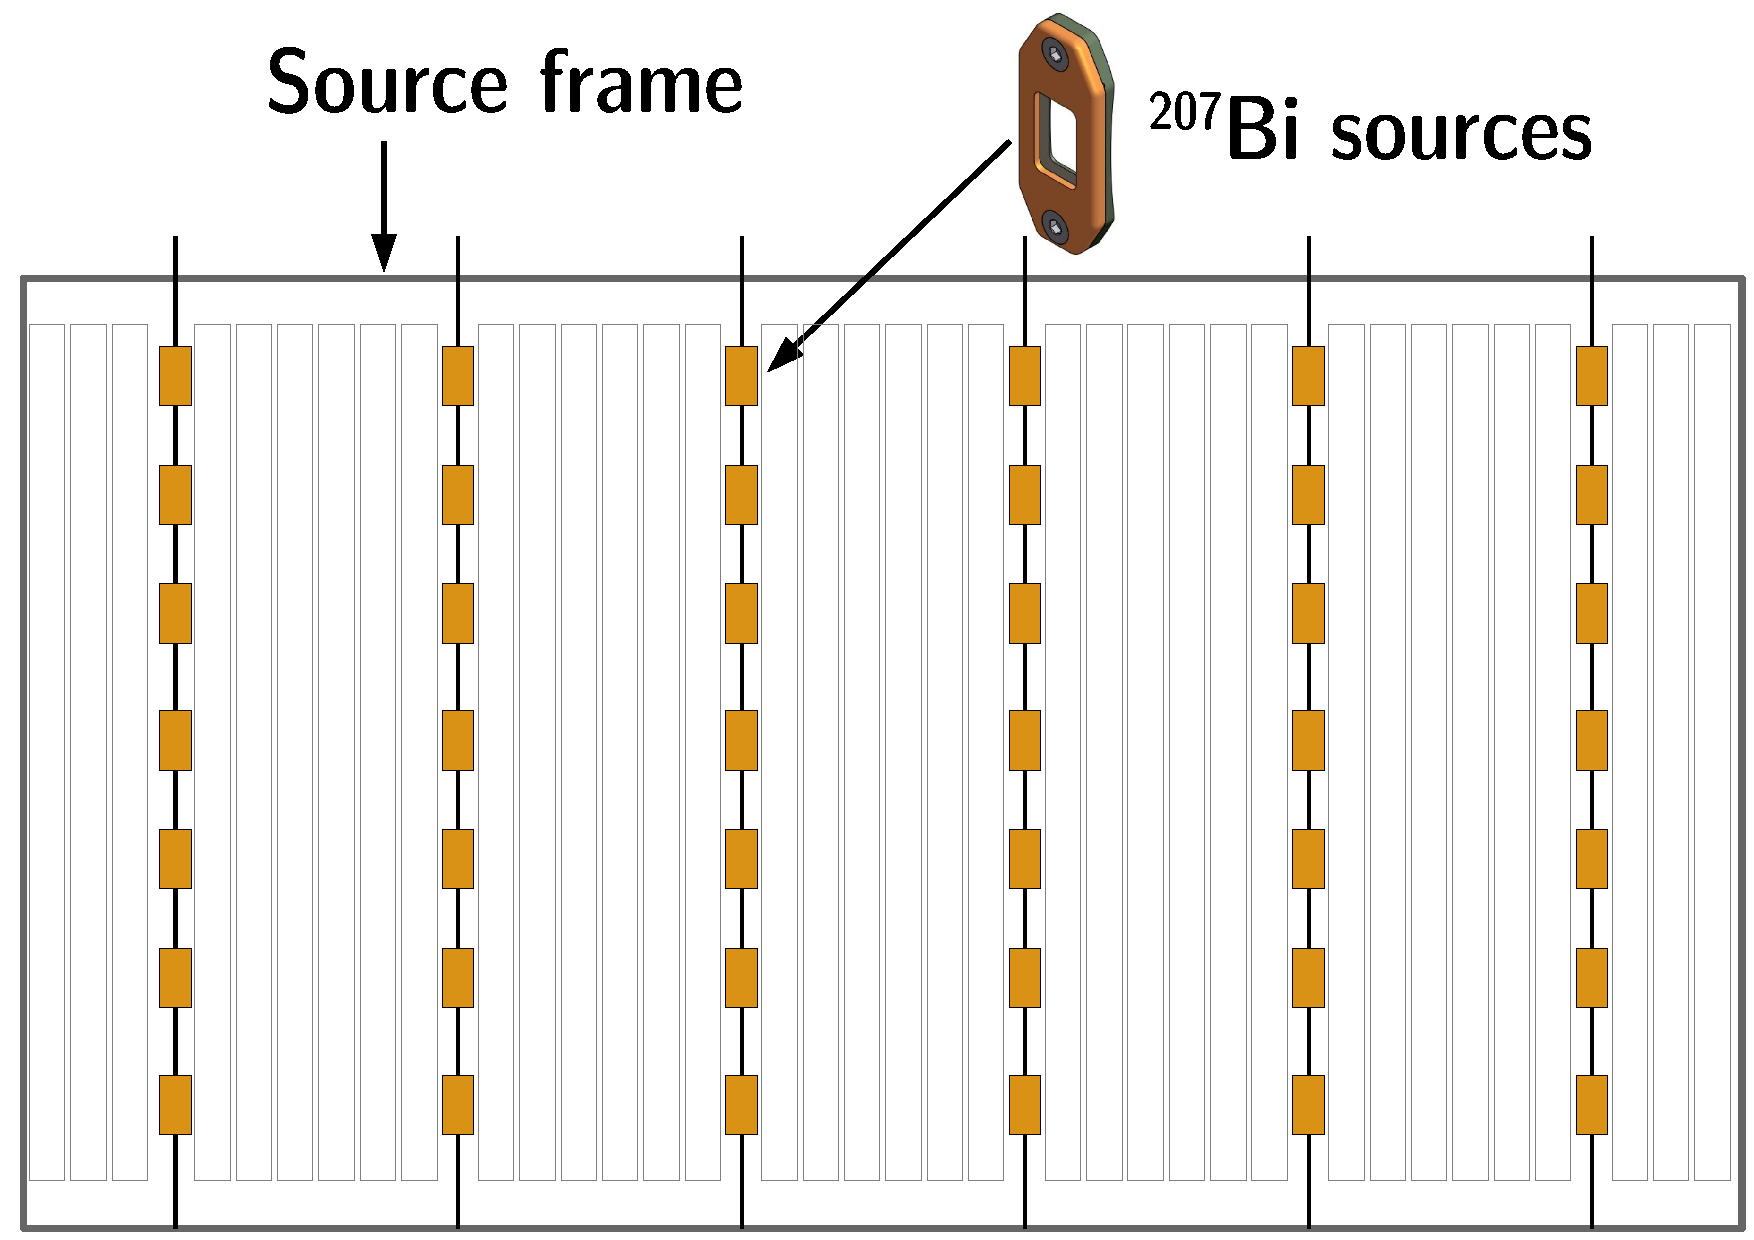
\includegraphics[height=0.8\textwidth]{SNdemonstrator/fig_SNdemonstrator/bi_sources_position.pdf}
  \end{subfigure}
  \hfill
  \begin{subfigure}[t]{0.49\textwidth}
    \centering
    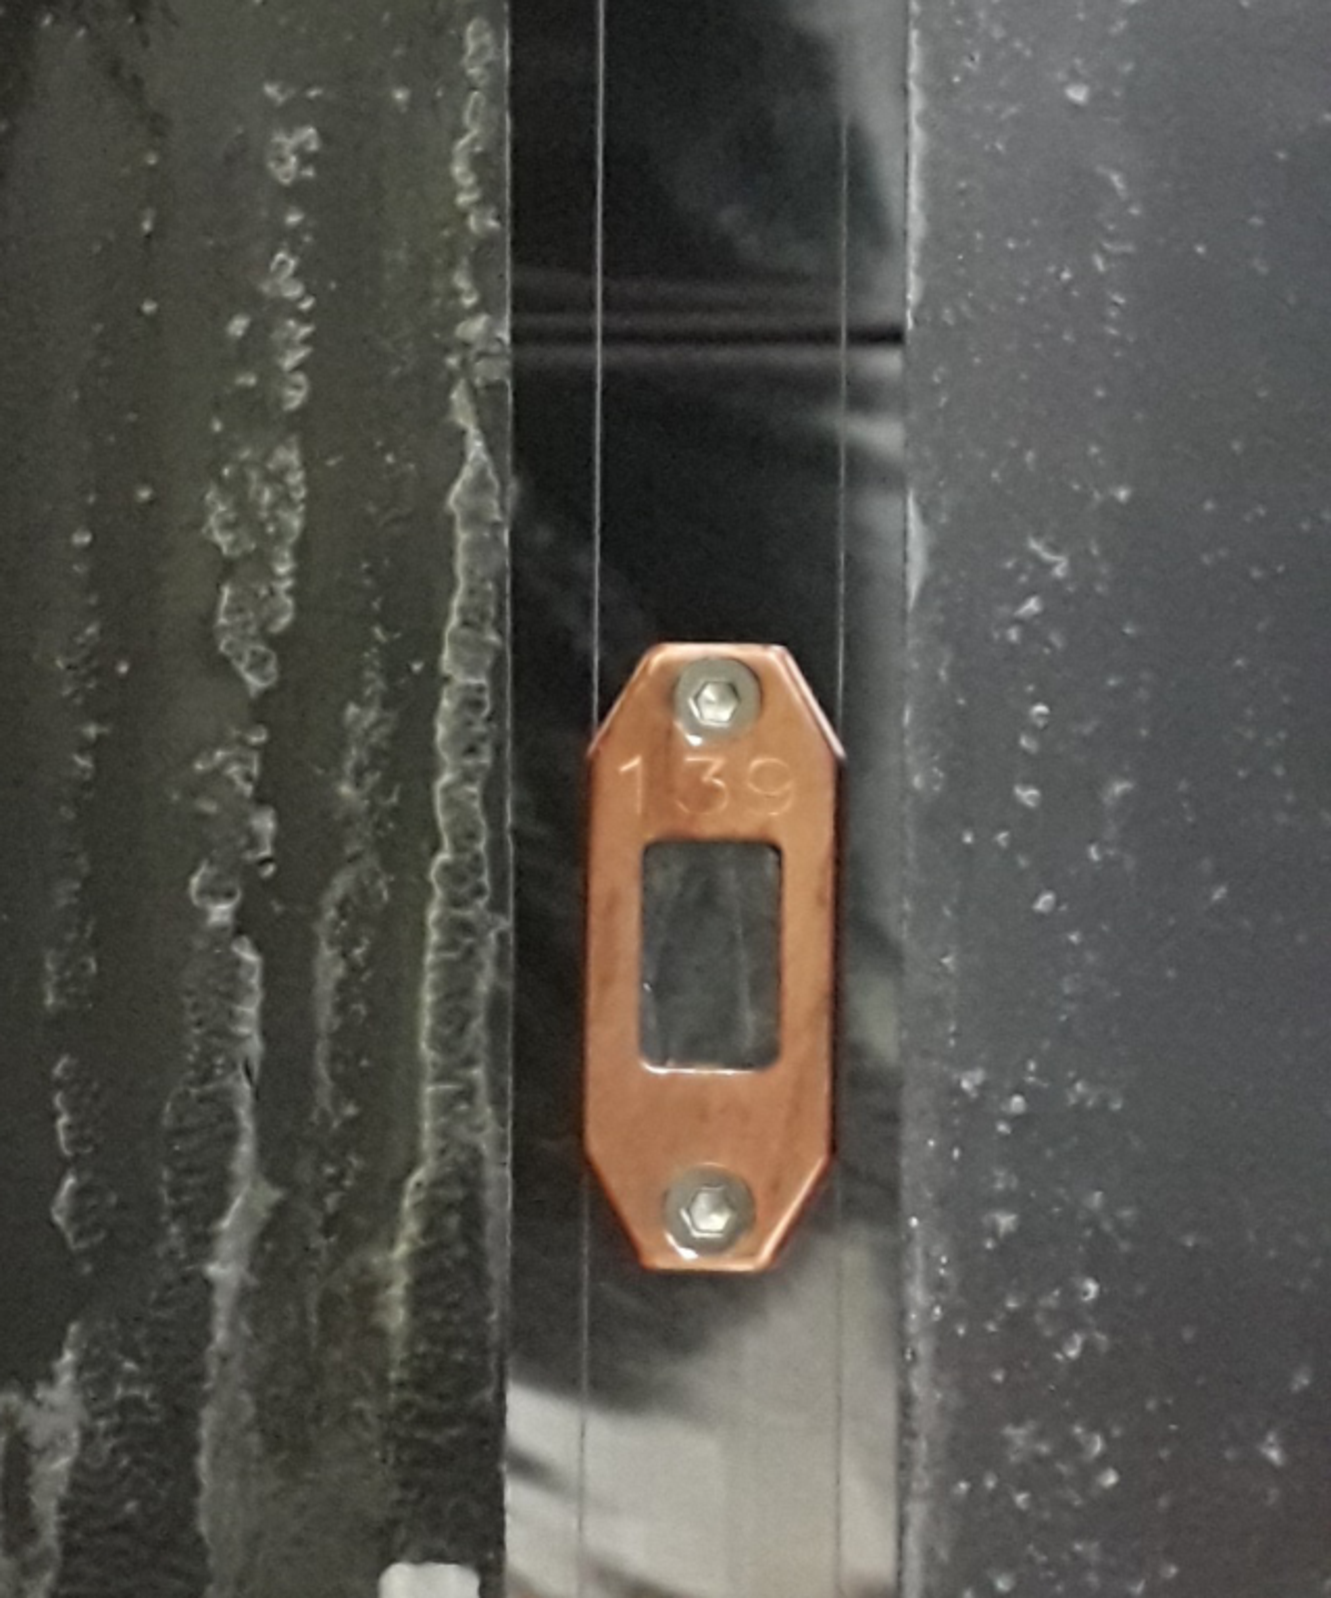
\includegraphics[height=0.8\textwidth]{SNdemonstrator/fig_SNdemonstrator/bi_source_pic.pdf}
  \end{subfigure}
  \caption{\Bi\ calibration sources in the automatised deployment system.
    Sketch of the sources deployed (left) and picture of one of the sources, between two ITEP source foils (right).
    \label{fig:bi_sources}}
\end{figure}

\subsubsection*{Light Injection System}


The so-called \emph{Light Injection} (LI) System will monitor the stability of the calorimeter response in energy during the data acquisition time ($\sim2.5$~years).
A scheme of the complete LI calibration system is given in Fig.~\ref{fig:LIS_scheme}.
Twenty Light Emitting Diodes (LED) at $385$ nm will inject light in each scintillator block via optical fibers.
A set of reference optical modules, receiving light from both LEDs and $^{241}$Am sources, monitors the stability of the LEDs.
This system is fully installed and entered in the commissioning phase in $2019$.
I participated in the analysis of the first LIS commissioning data taken discussed in Chapter~\ref{ch:commissioning}.
\begin{figure}[h]
  \centering
  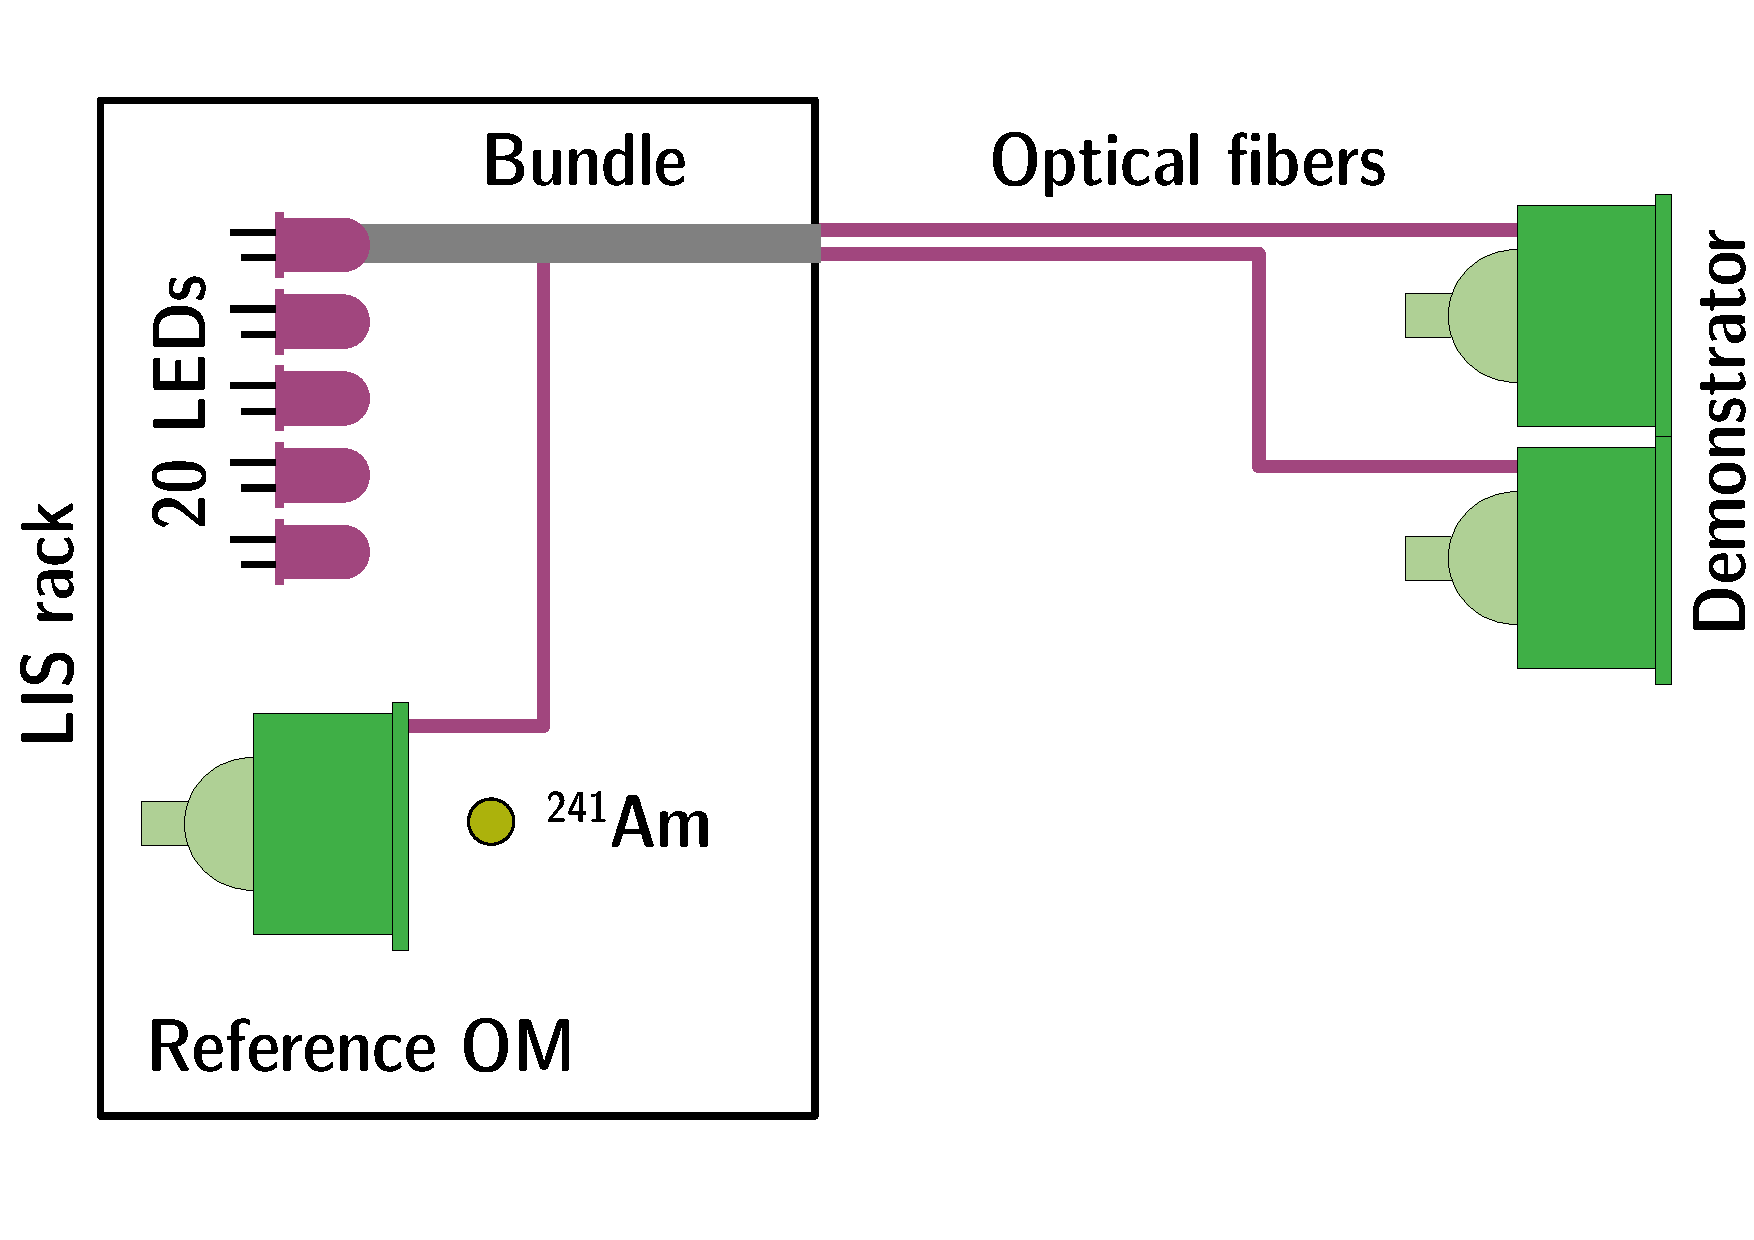
\includegraphics[width=10cm]{SNdemonstrator/fig_SNdemonstrator/LIS_scheme.pdf}
  \caption{A scheme of the Light Injection (LI) calibration system.
    More than $1300$ fibers, distributed in $20$ bundles, carry the light from $20$ LEDs to each scintillator block of the demonstrator.
    Reference OMs coupled with $^{241}$Am sources monitor the LED light.
    \label{fig:LIS_scheme}}
\end{figure}


\subsection{Detector cabling}

During the R\&D program, special attention has been paid to the total number of electronic channels needed for the demonstrator.
Indeed, this number must remain reasonable in order to control the total cost of the experiment, but must be high enough so that the granularity of the detector is sufficient to search for the $\zeronu$ decay.
Indeed, a good background events rejection where two electrons and a gamma particle are emitted can be ensured if they are detected in different optical modules.

Ultimately the detector will be enclosed in an anti-radon tent, which is described in Sec.~\ref{subsec:background_reduc}.
In order to ensure that this external envelope is leak-tight, a patch panel (PP) has been designed to allow cables to pass the tent, from the inside to the outside.
Cables coming from the detector, called \emph{internal cables}, are connected to a specific location on the patch panel.
So-called \emph{external cables} are connected on the other side and allow the signal transmission to electronics.

\subsubsection*{Calorimeter cabling}

The basic operation principle of a SuperNEMO photomultiplier has been discussed in Sec.~\ref{subsec:SN_calo}.
For this sub-detector to amplify the signal a potential difference is applied between its dynodes.
To do so, a high voltage (HV) must be provided to the PM.
Therefore, each PM divider is connected to a so-called \emph{high voltage} cable.
The voltage applied depends on the individual optical module characteristics and is about $\sim1500$~V for the $8$~inches and $\sim1100$~V for the $5$~inches.
After the electrons have reached the last dynode, the charge is transported by \emph{signal cables} to the electronics.
Finally, each PM divider is connected to two cables, one for the high voltage and one for the signal.
A back view of one of the fully cabled main calorimeter wall is given in Fig.~\ref{fig:calo_cabling_pic}.
\begin{figure}[h]
  \centering
  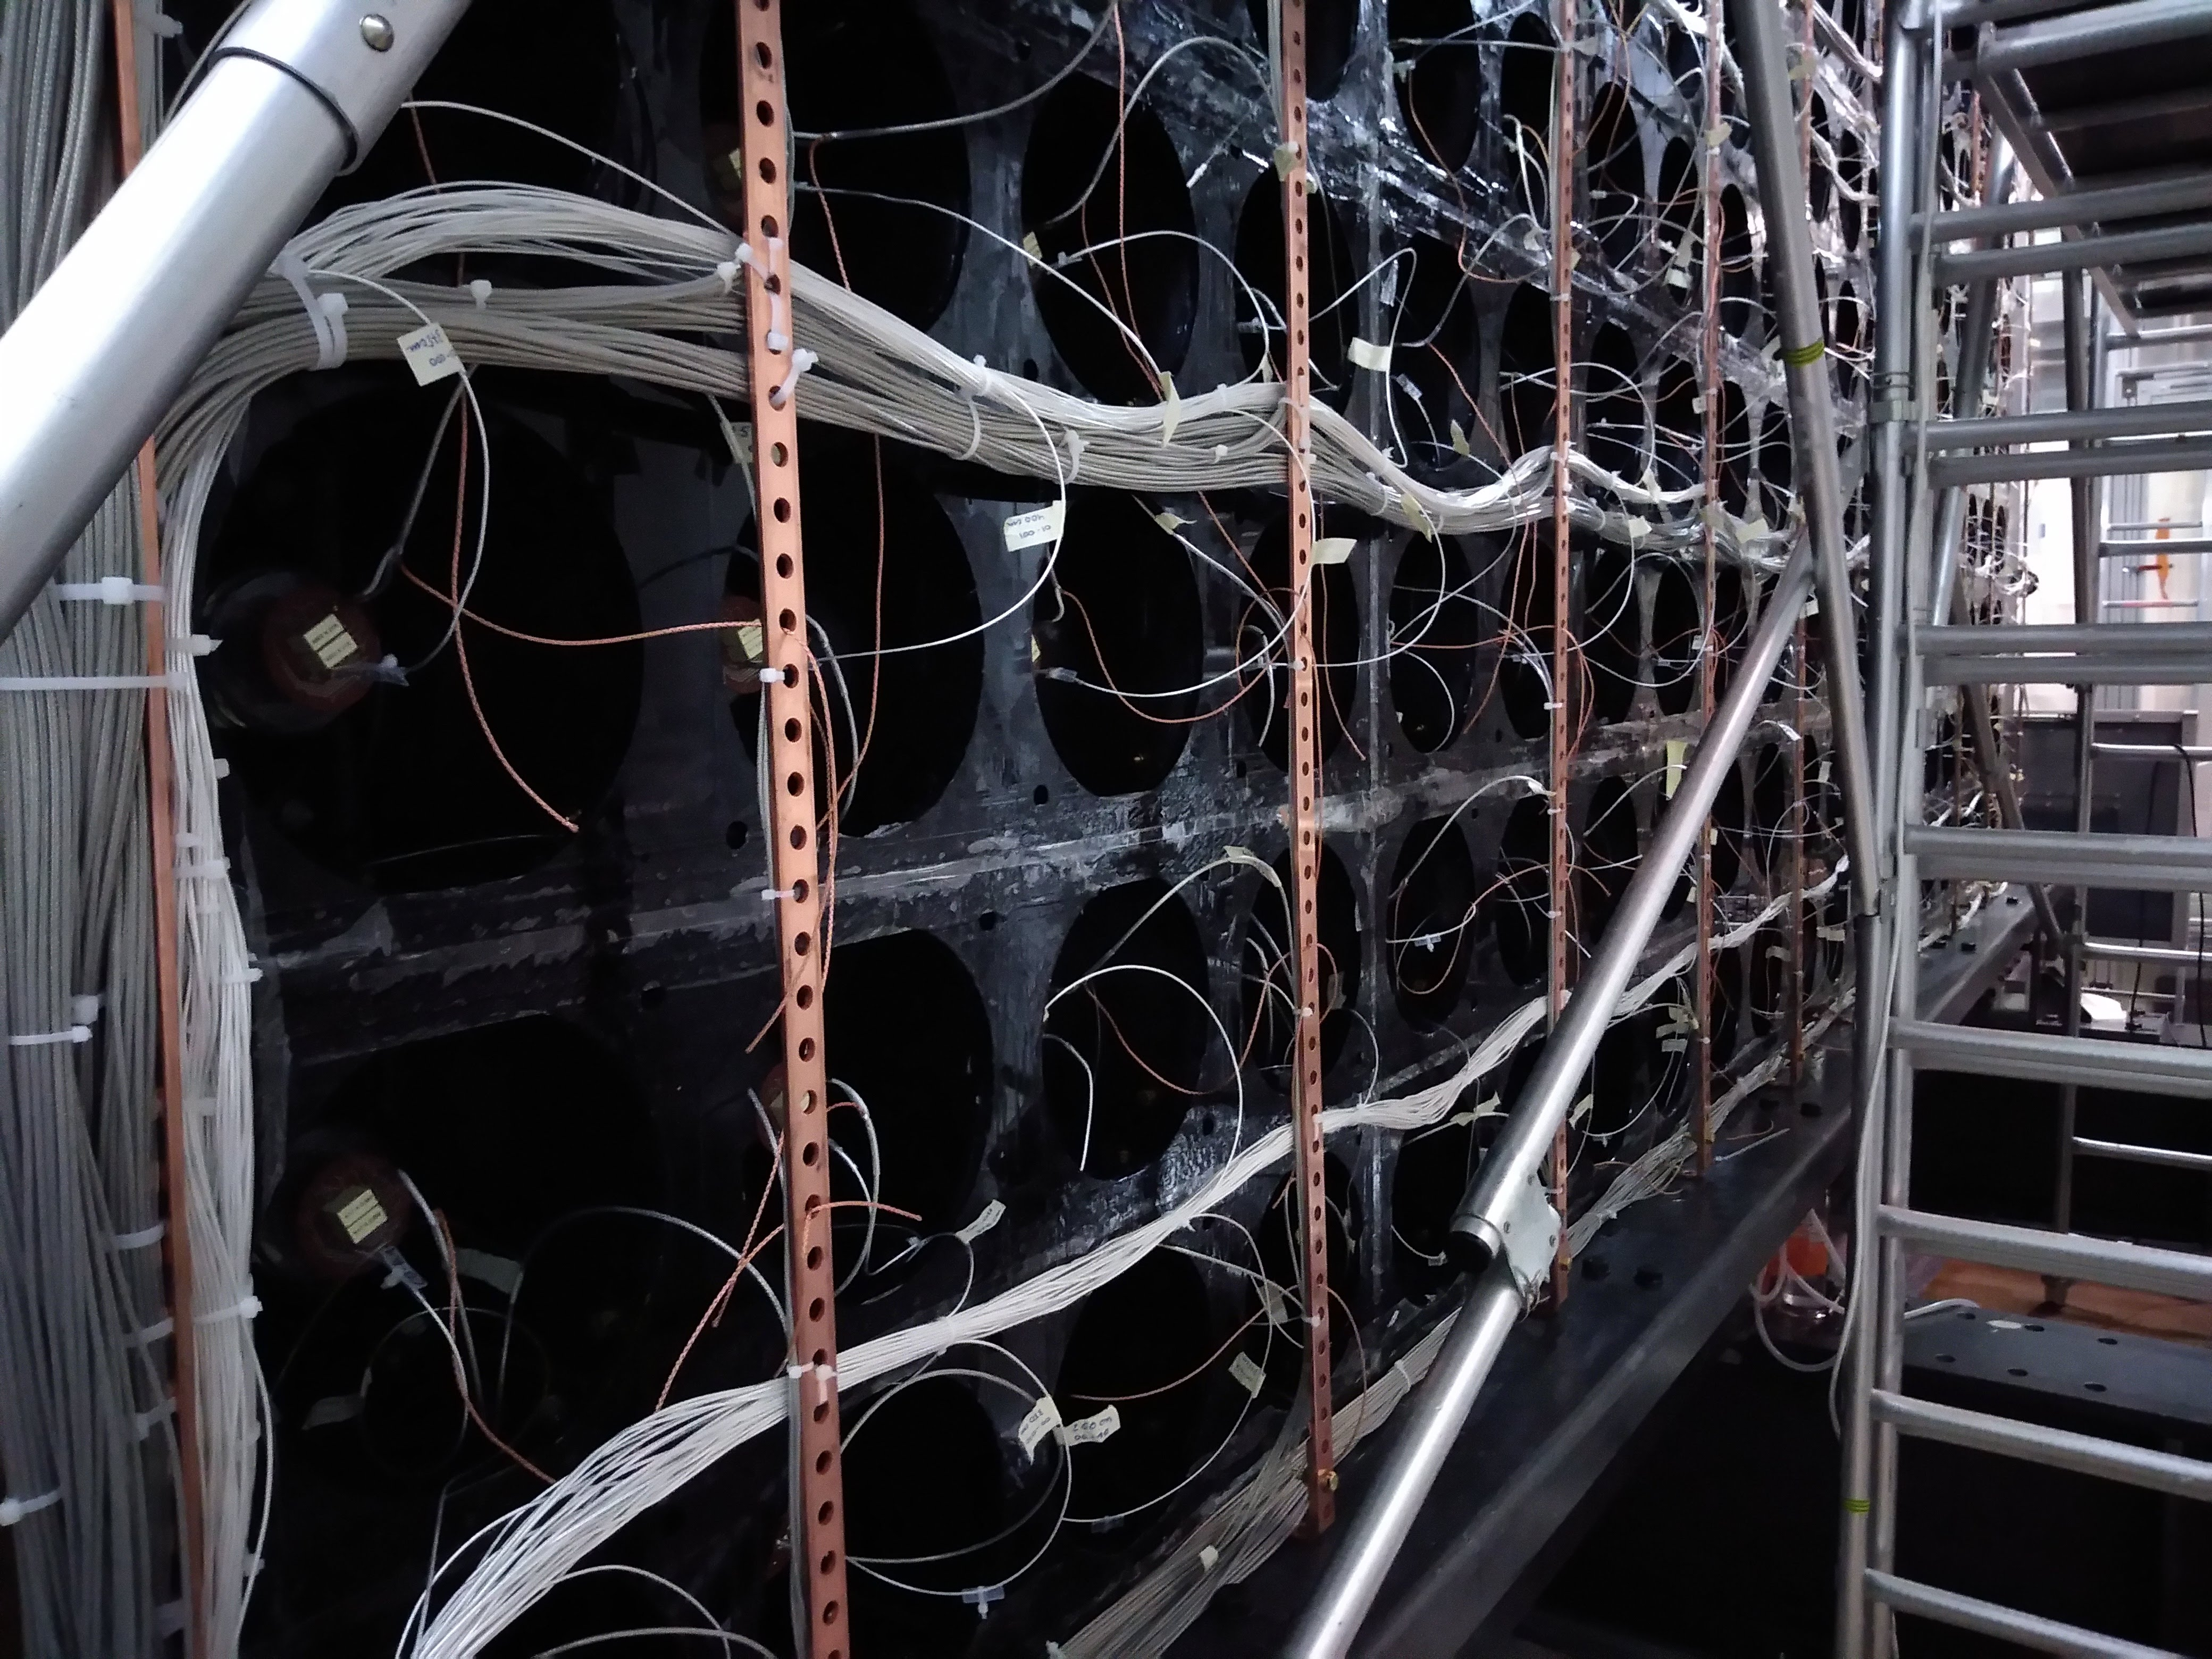
\includegraphics[width=0.8\textwidth]{SNdemonstrator/fig_SNdemonstrator/cable_calo_pic.pdf}
  \caption{Back view of one main calorimeter wall.
    Signal cables are white and thin, HV cables are grey and thick.
    \label{fig:calo_cabling_pic}}
\end{figure}

A global sketch of the calorimeter cabling is given in Fig.~\ref{fig:calo_cabling}, picturing all internal, external, high voltage and signal cables.
External HV cables are grouped in $26$ bundles, and each HV channel corresponds to a given pin on the bundle connector.
External signal cables are independently routed from patch panel to electronics, as it is the case for internal HV and signal cables.
\begin{figure}[h]
  \centering
  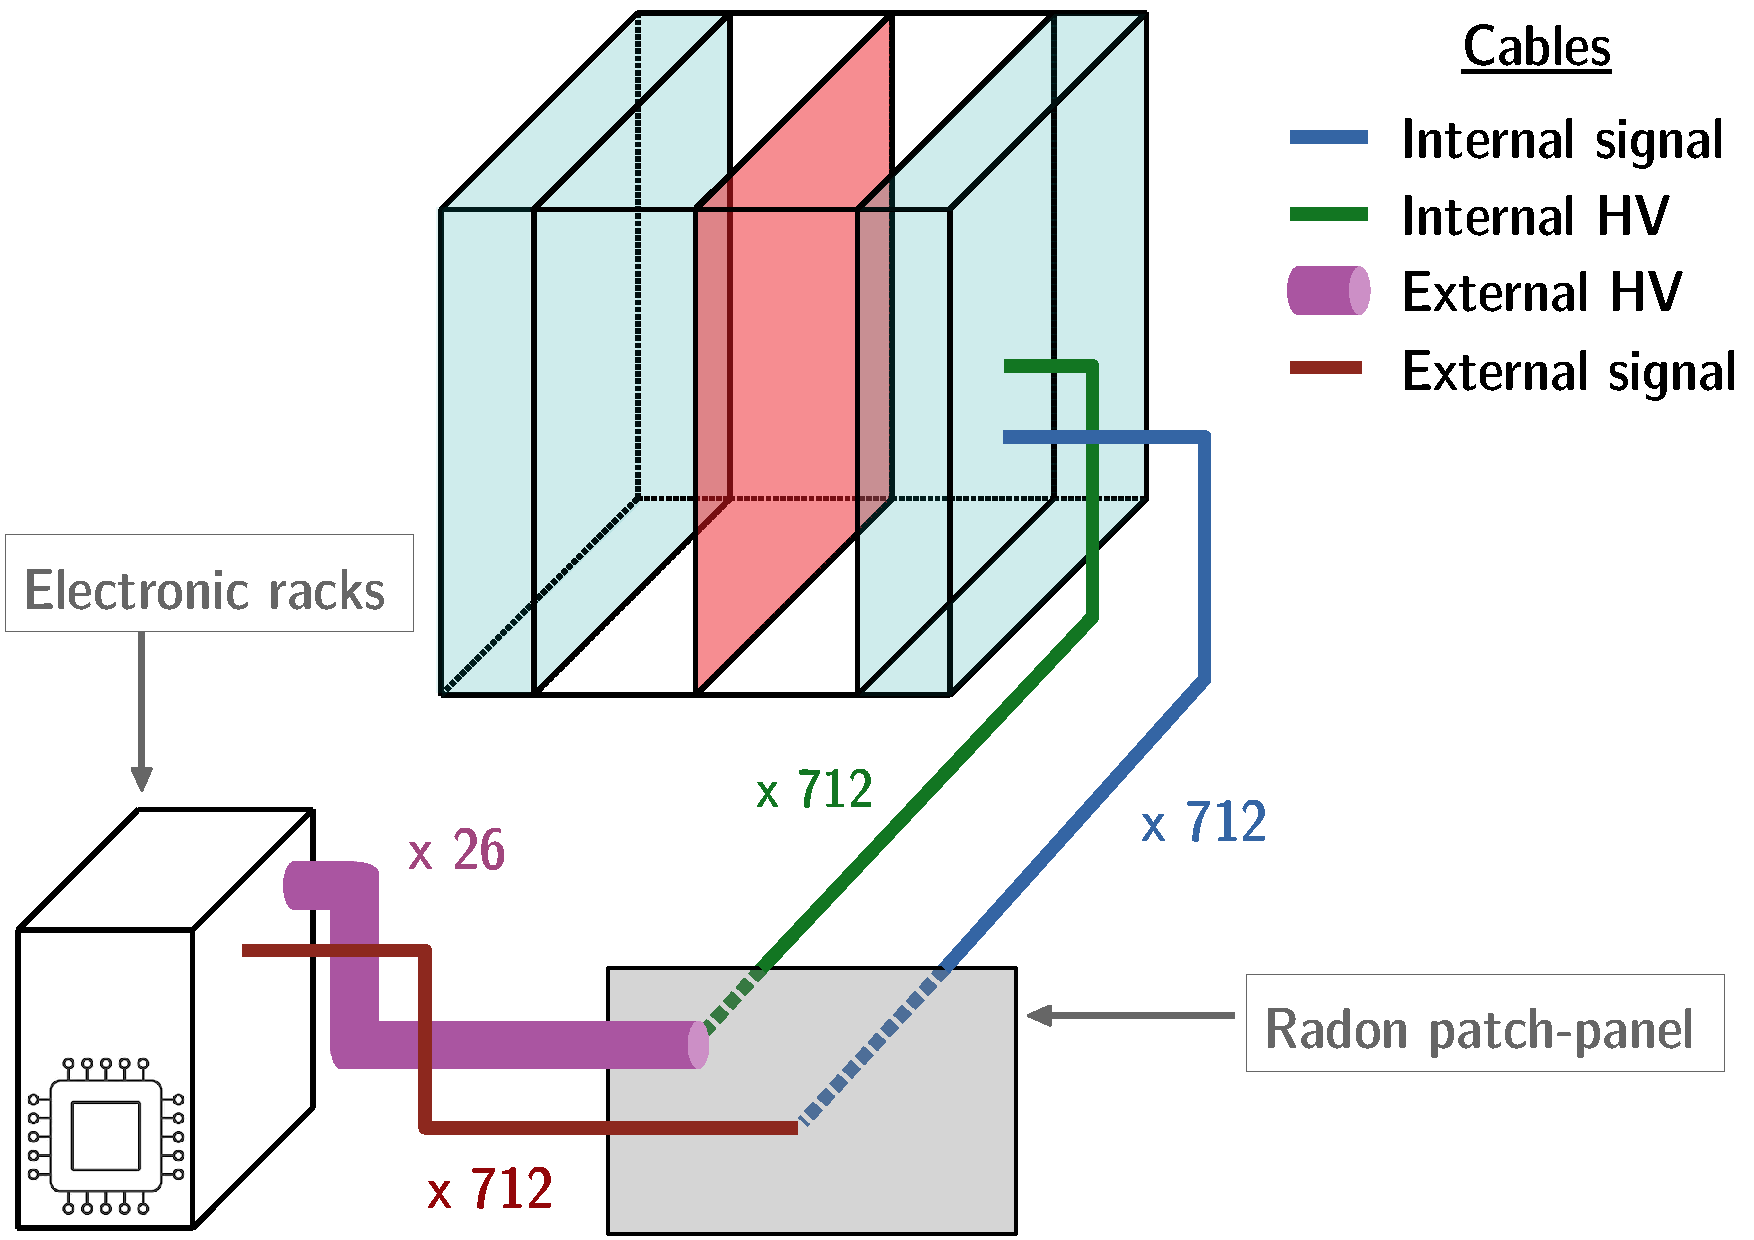
\includegraphics[width=0.9\textwidth]{SNdemonstrator/fig_SNdemonstrator/calo_cabling.pdf}
  \caption{A scheme of the calorimeter cabling.
    Internal signal and HV cables go from the calorimeter to the patch-panel.
    External cables link the patch-panel to the electronic racks.
    \label{fig:calo_cabling}}
\end{figure}

\subsubsection*{Tracker cabling}

The same internal and external pattern applies to the tracker cables.
Geiger cells are connected via cables to the patch panel, where external cables, several tens of metres long, are linked to the electronics.

The routing of tracker and calorimeter lasted several months and required an enormous amount of work and involvement from the whole of the collaboration.

\subsection{Electronics}

Dedicated electronics has been developed for the SuperNEMO demonstrator.
Six racks arranged next to the detector contain all it.
The racks have been organised in separate areas - called crates - to accommodate the hardware dedicated to the calorimeter, tracker and calibration systems.
The calorimeter electronics were realised at LAL while the tracker electronics were developed jointly by the French and English teams.

The triggering and acquisition electronics are based on a three-levels architecture: the front-end boards (FEB), the control boards (CB) and the trigger boards (TB).
From the analogue signal generated in one part of the detector to its storage, a complex communication pattern takes place between these three structures.
\begin{enumerate}
\item The FEBs receive, process and digitise the primary analogue signals from the optical modules and the Geiger cells.
  The digitisation of the pulses by the FEBs is an innovation for SuperNEMO compared to NEMO-$3$ where only the ADC (analogue-to-digital converter) and TDC (time-to-digital converter) were calculated.
  This would permit to distinguish two successive interactions in the same electronic pulse.
  Part of this information is transmitted directly to the control board.
  Other data are stored in the FEBs as long as the central controller system has not validated or invalidated their acquisition.
  There are two types of FEBs, one for the calorimeter and one the tracker.
\item The control boards receive, centralise and forward signals coming from distinct locations of the detector (i.e. distinct FEBs).
  The calorimeter and tracker control boards have the same design and only differ by the firmware.
\item Once the acquisition decision is taken by the trigger board, the control boards propagate the information to calorimeter and tracker FEBs for the acquisition to begin.
\item After the acquisition has been taken, all digitised data are sent via the control boards to the data acquisition system (DAQ).
\end{enumerate}
The electronics commissioning has begun in June $2018$ at Manchester and is fully completed.
I participated in the timing calibration of the front-end boards, which I discuss in Chapter~\ref{ch:commissioning}.

\subsubsection*{Dedicated calorimeter electronics}

In total, three crates are dedicated to the signal acquisition of the calorimeter.
Each of them houses $20$ front-end boards and one control board placed in the centre of the crate.
A picture of one fully cabled calorimeter crate is given in Fig.~\ref{fig:calo_crate}.
All the photomultipliers of a calorimeter wall are connected to front-end boards of a unique crate.
Each front-end board collects the output PM signals of one column of optical modules of the calorimeter wall.
\begin{itemize}
\item For each of the main walls, $20$ front-end boards are needed, each board corresponding to $13$ output PM signals.
\item For X-Walls and Gamma-Vetos, only $12$ front-end boards are needed ($8$ for X-Walls and $4$ for Gamma-Vetos).
  One front-end board corresponds to $16$ output PM signals.
\end{itemize}
In total, all the $52$ FEBs needed for the calorimeter electronics were designed at LAL with $16$ channels each, collecting all the signals from the $712$ optical modules.
\begin{figure}[h]
  \centering
  \includegraphics[width=0.8\textwidth]{SNdemonstrator/fig_SNdemonstrator/calo_crate.pdf}
  \caption{Picture of a calorimeter crate for one of the main wall.
    \label{fig:calo_crate}}
\end{figure}

\subsubsection*{Dedicated tracker electronics}


Three crates are dedicated to the tracker electronics, with $680$ Geiger cells per crate (for a total of $2040$ cells).
In each crate, there are $19$ tracker front-end boards, called tracker FEBs.
Each FEB therefore contains $108$ electronic channels.
A control board is located in the centre of each crate and centralises the information from the FEBs.
A total of $57$ FEBs and $3$ CB are then needed to collect the signal of all the anodic and cathodic analogue signals from the wire chamber.

\subsubsection*{Calibration racks}

Two racks are dedicated to the electronics and informatics of the demonstrator's calibration systems (one for the deployment system, one for the light injection system).


\subsection{Detector gas tightness}
\label{subsec:sealing}


An important part of the SuperNEMO detector is filled with a Helium-based gas mixture.
As described in Sec.~\ref{subsec:tracker} it is essential for the proper functioning of the tracker that the detector is gas tight.
As with the NEMO-$3$ detector, a major effort is therefore made to ensure that the detector is sealed to prevent external contaminants from infiltrating.
Different techniques are deployed during and after the detector assembly (Fig.~\ref{fig:sealing_plan}).
\begin{itemize}
\item The pre-assembled blocks of $8$ optical modules were wrapped in a radio-pure nylon film.
  Additional patches of nylon film were glued on the calorimeter back side on each gap between these groups of $8$ optical modules.
\item After the calorimeter walls assembly, copper bars have been installed on the back side at the gap between the calorimeter and the structure supporting the detector.
\item A piece of nylon was mounted on the front side of each main wall before the detector was closed (Fig.~\ref{fig:nylon_film}) in order to prevent the Radon from emanating from the calorimeter to the tracker.
\item Different leak-sealing radio-pure materials (SBR, RTV, Stycast and Black Mamba glues) have been applied on different detector areas (mainly inside the optical module shieldings, tracker frame and source frame).
\end{itemize}
I took part in several of these operations, and my first shift to Modane was one of them.
\begin{figure}[h!]
\centering
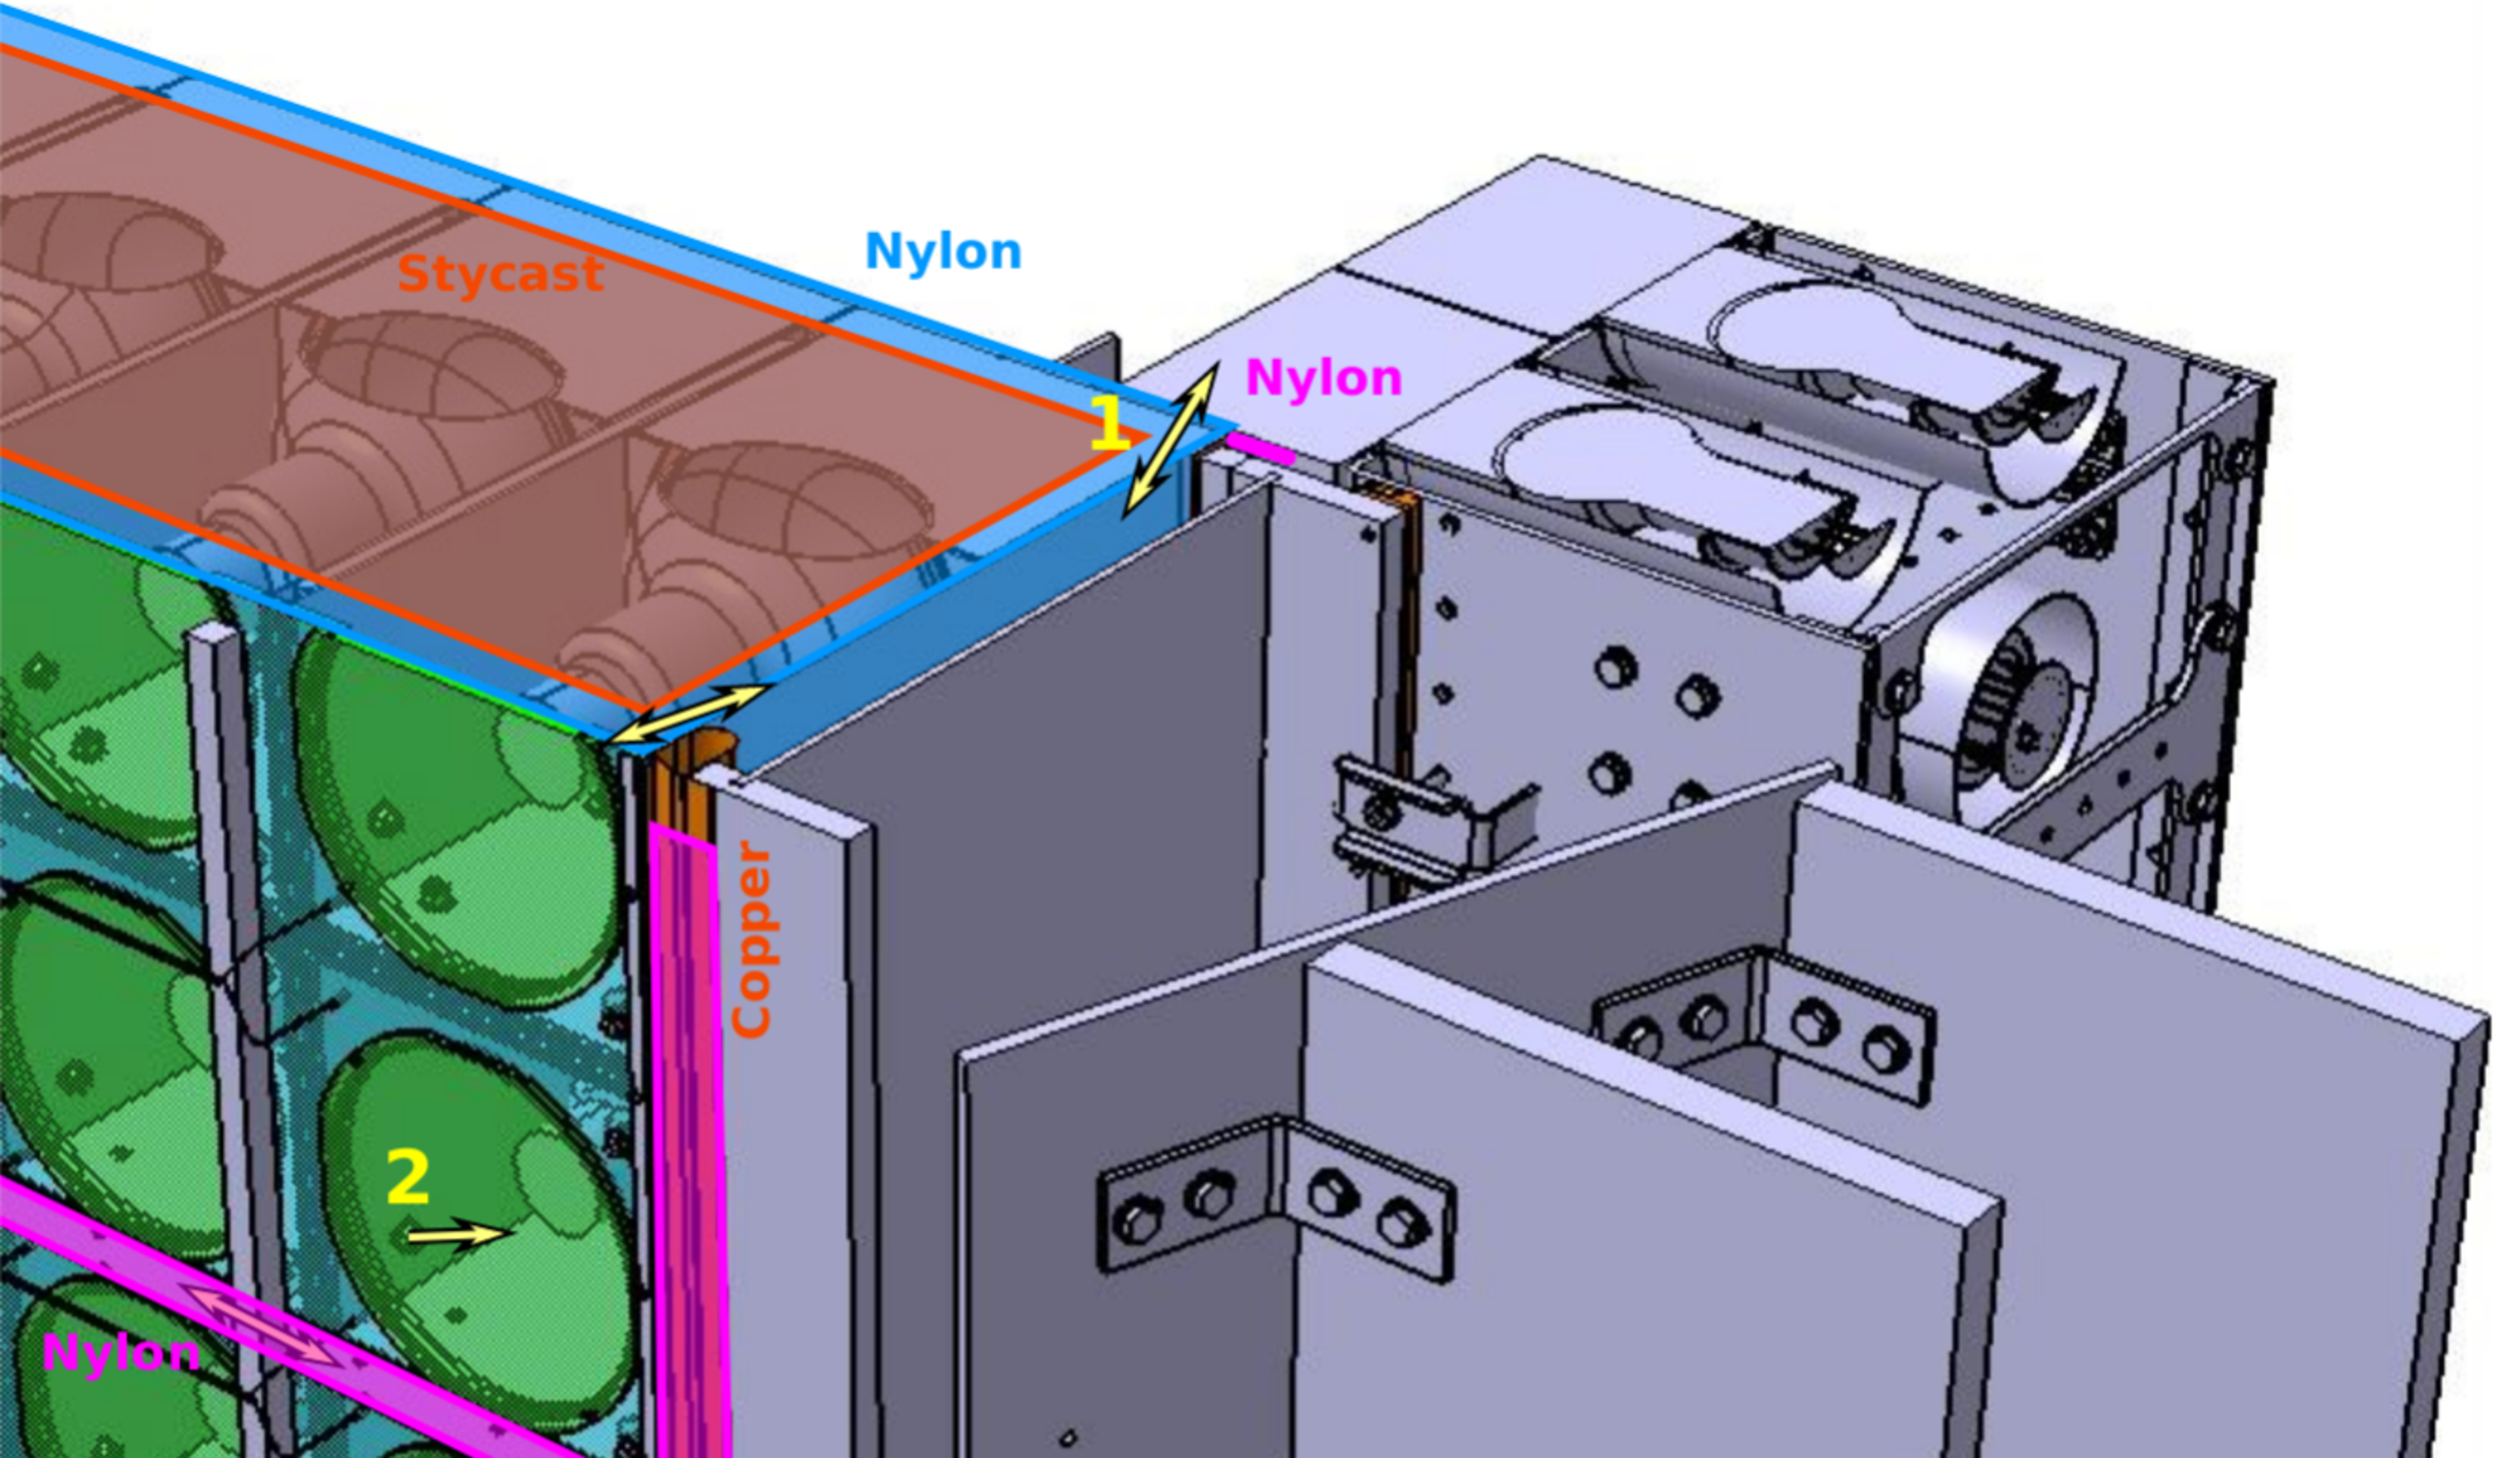
\includegraphics[width=0.8\textwidth]{SNdemonstrator/fig_SNdemonstrator/leaks.pdf}
\caption{Demonstrator gas tightness plan.
  Back view of one of the calorimeter main walls.
\label{fig:sealing_plan}}
\end{figure}
\begin{figure}[h!]
\centering
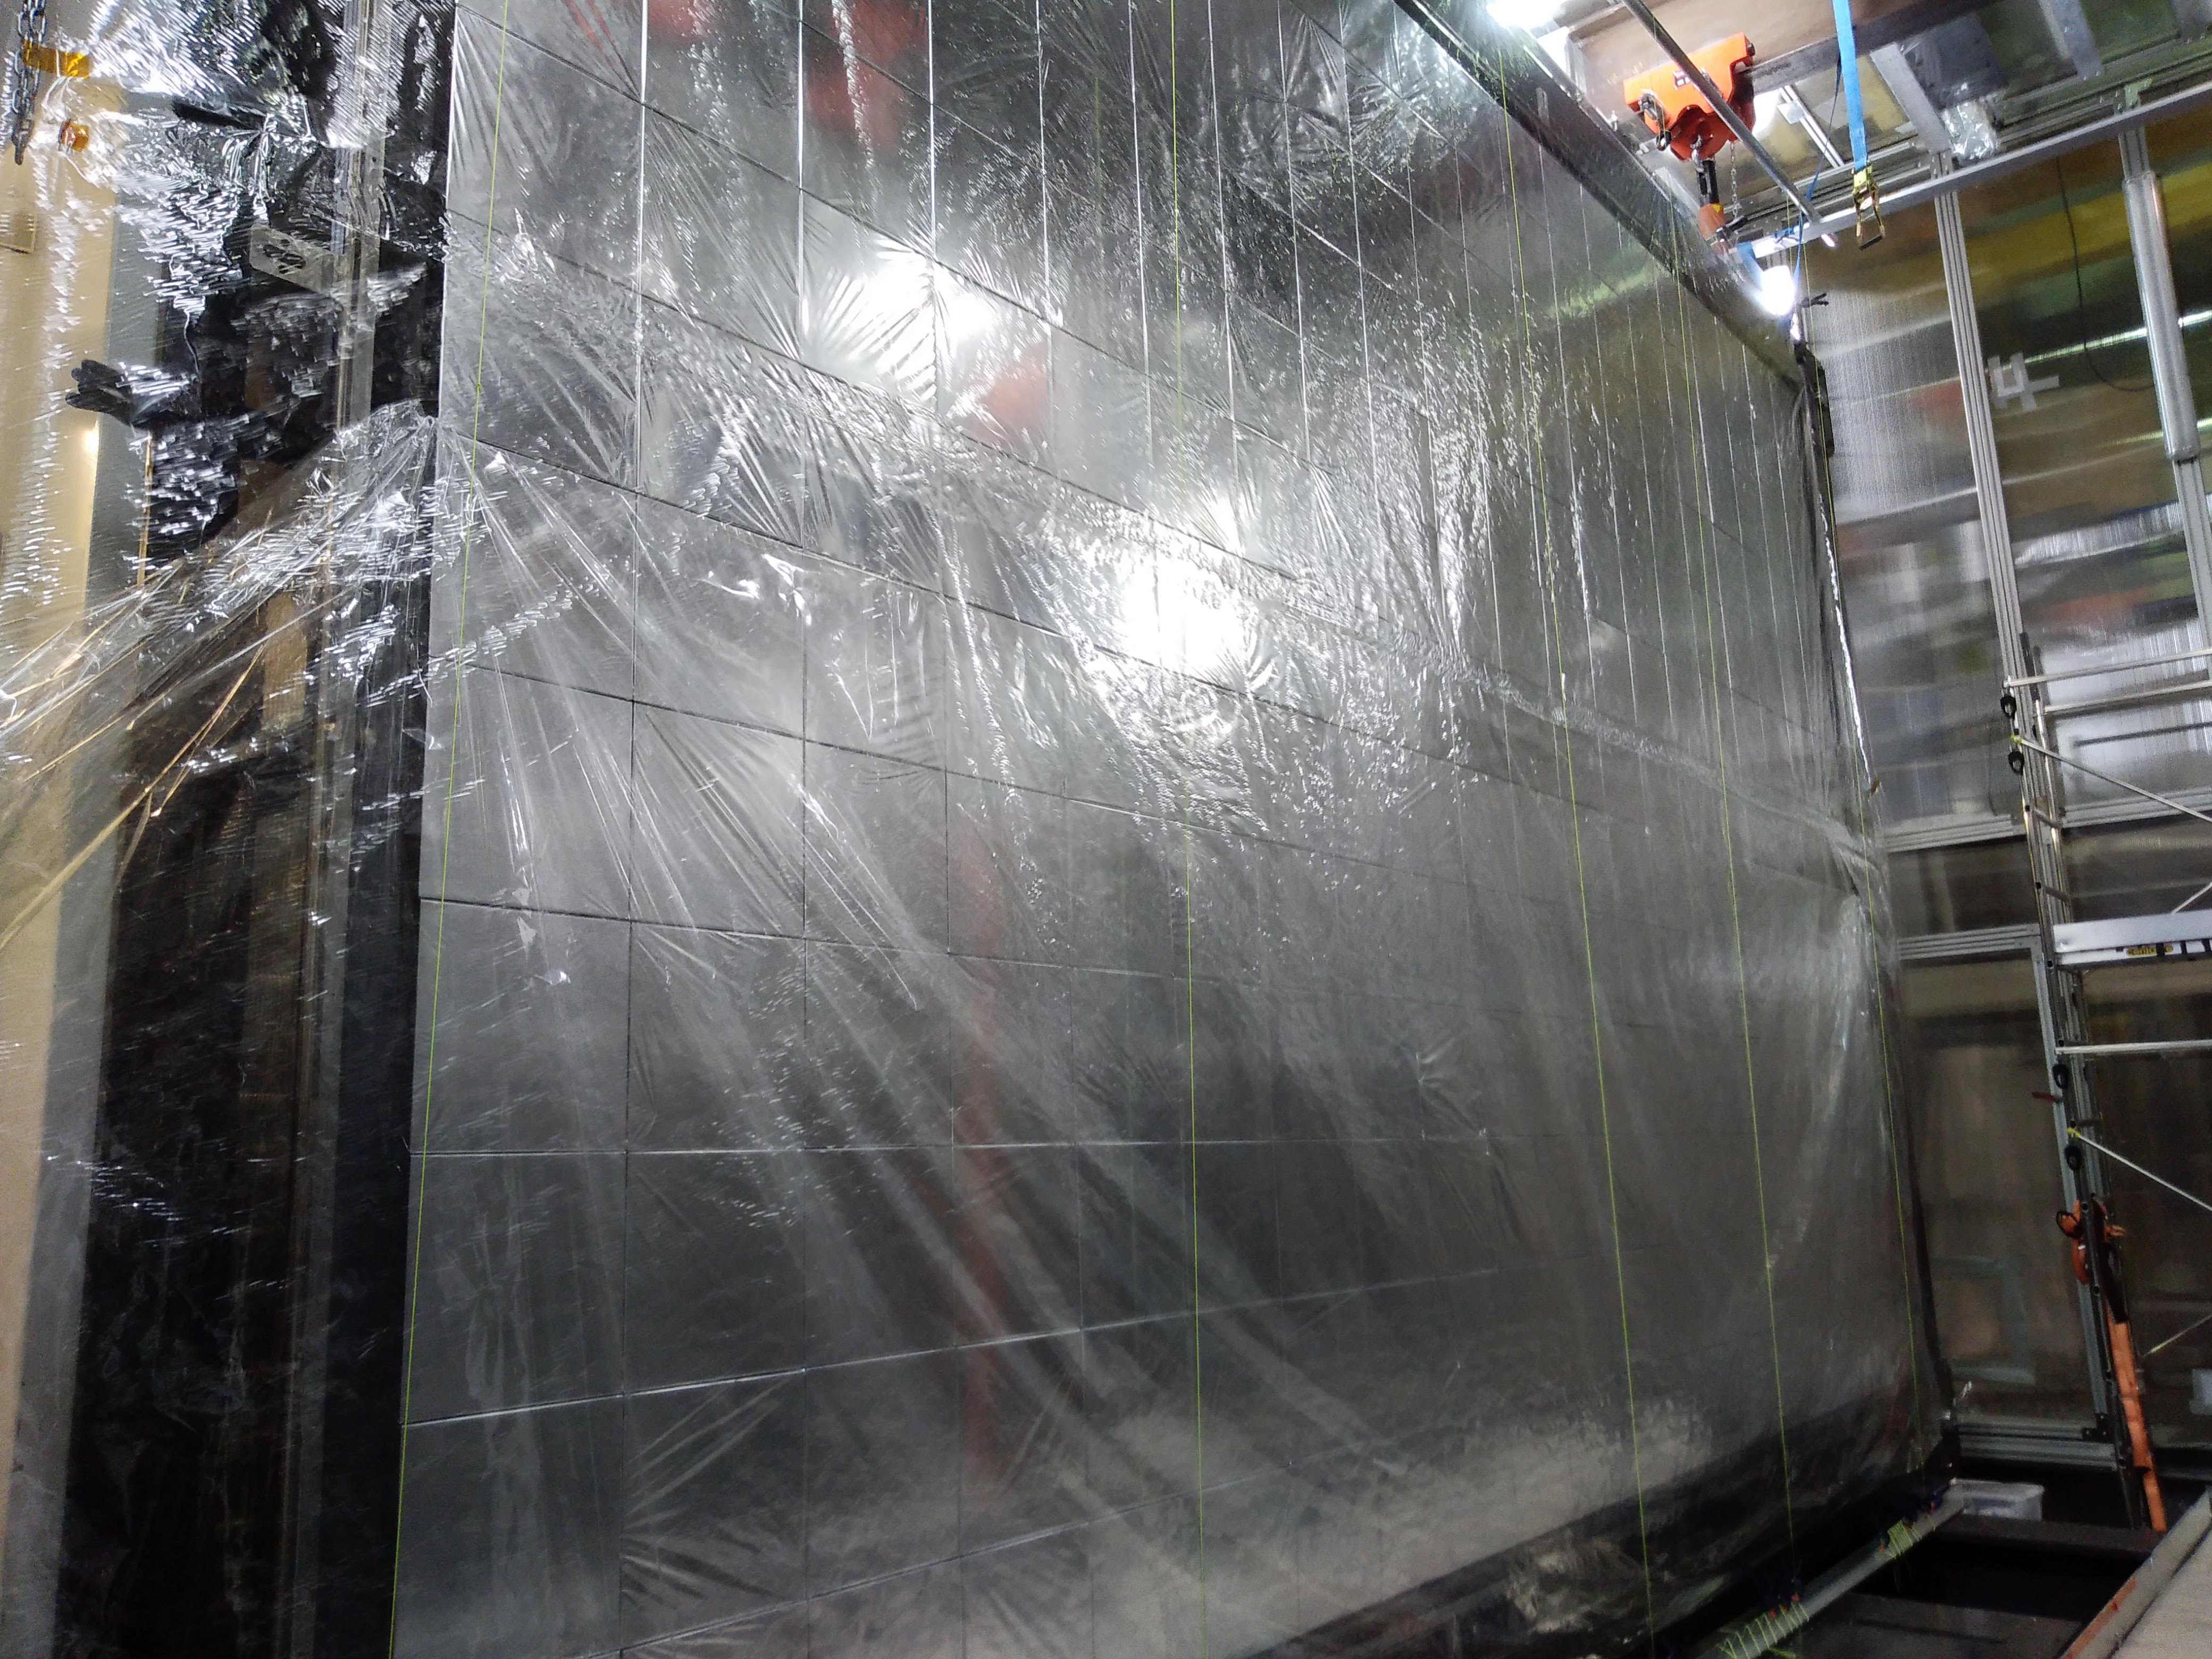
\includegraphics[width=0.8\textwidth]{SNdemonstrator/fig_SNdemonstrator/Nylon_film.jpg}
\caption{Piece of radio-pure nylon film installed on the front face of each calorimeter main walls.
\label{fig:nylon_film}}
\end{figure}

After these operations, remaining leaks can still occur through two interfaces:
\begin{itemize}
\item through the nylon film.
  Indeed, one of the two films (Italian side) was damaged during the detector closure leading to possible gas leaks between the tracker volume and the optical modules buffer volume,
\item through optical module magnetic shieldings (in the area of the clamping screws) leading to leaks between the buffer volume and the detector outside.
\end{itemize}
In order to reduce these leaks, several sealing operations have been carried out.
They consist in injecting a gas inside the tracker via the gas injection system and detect possible leaks with a gas probe.
In case of major leaks, helium gas could infiltrate the PMs vacuum by diffusing through the glass.
Therefore the gas chosen for the first leaks checks is Argon.
Every major leak is then fixed using the more suitable radio-pure glues presented above (depending on the size and location of the leak).
The first over-pressure in the tracker was successfully obtained in September $2019$ showing that a reasonable gas-tightness was achieved.
After all major leaks were detected, Helium can be injected inside the tracker to identify smaller leaks without any danger for the PMs.

%% \begin{figure}[h!]
%% \centering
%% 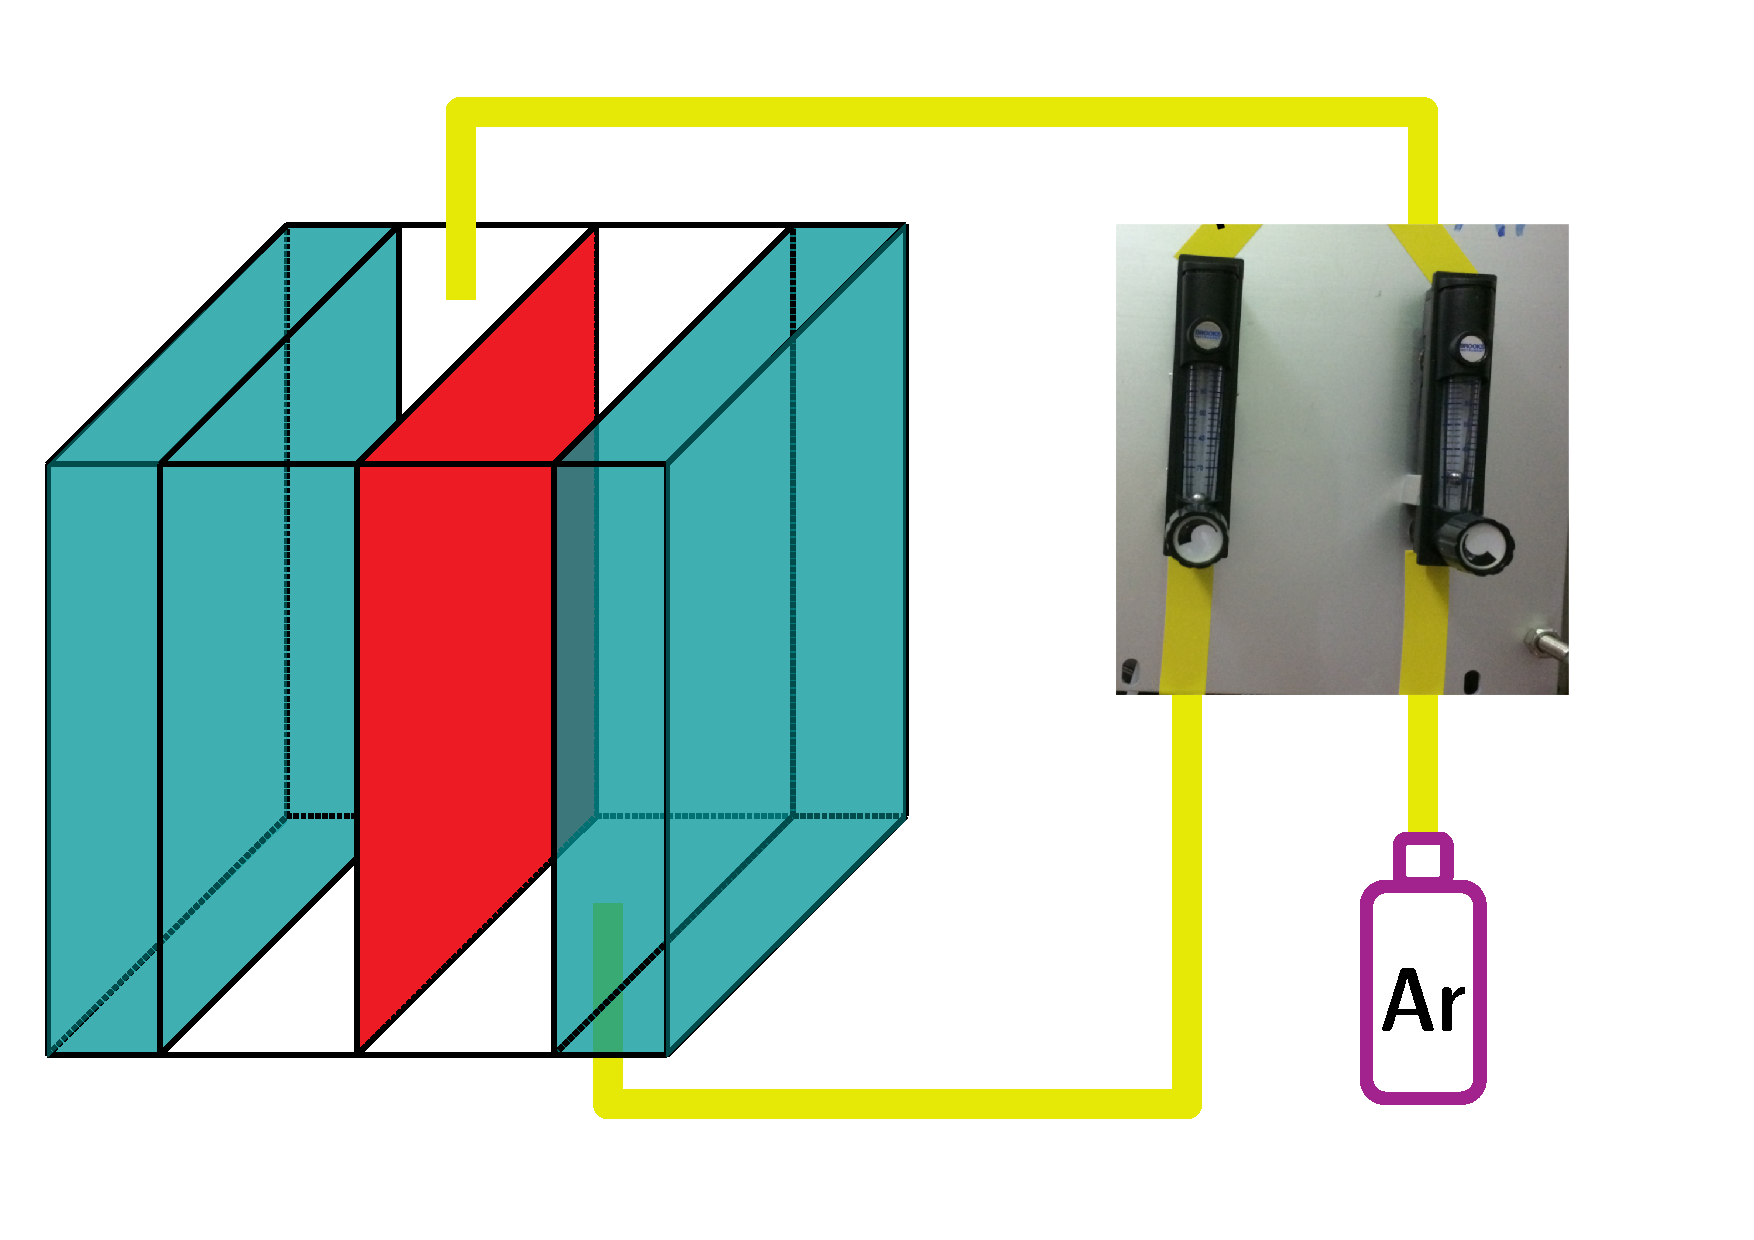
\includegraphics[width=0.6\textwidth]{SNdemonstrator/fig_SNdemonstrator/gas_tightness.pdf}
%% \caption{Leak checking procedure.
%%   A sketch of the demonstrator on the left, with calorimeter (blue), tracker (colourless) and source (red).
%%   A heavy gas (Argon) is sent inside the wire chamber.
%%   The gas pressure is then check inside the tracker.
%% \label{fig:}}
%% \end{figure}


%which glues used? (RTV (radon permeable), SBR (radon tight), stycast, black mamba, )\\

\section{Backgrounds}
\label{sec:SNbkg}

The SuperNEMO experiment seeks, if it exists, an extremely rare signal.
It is therefore necessary to know and reduce as much as possible the possible sources of background that could degrade the observation of the signal in question.
The energies involved in the double beta process imply that this type of experiment is sensitive to several sources of background.

\subsection{Internal background}
\label{subsec:SNbkg_internal}

We refer to \emph{internal background} as the background being generated from inside the sources, where trace quantities of naturally-occurring radioactive isotopes can occasionally produce two-electron events and thus mimic $\beta\beta$-decay events.
The largest contributions come from isotopes of the natural decay chains of $^{238}$U and $^{232}$Th.

\subsubsection*{Two-electrons signature processes}

Following a beta disintegration, mainly three processes are likely to mimic a double beta disintegration with two electrons exiting the source foil as a signature, as shown in Fig.~\ref{fig:internal_contamination}.
\begin{itemize}
\item An electron resulting from an internal conversion is ejected from the atom in addition to the electron  beta.
An X-photon can also be emitted without being detected by the calorimeter.
This process will be described in detail in Chapter~\ref{ch:timediff}.
\item The initially emitted electron can scatter in the source on another electron through the so-called M\o{}ller scattering, and emit a second electron of significant energy.
\item The photon can eject an electron from the source by the Compton effect.
If the scattered photon is not detected in the calorimeter, this decay may present a two-electron signature.
\end{itemize}
\begin{figure}[!h]
\centering
\begin{subfigure}[t]{0.32\textwidth}
  \centering
  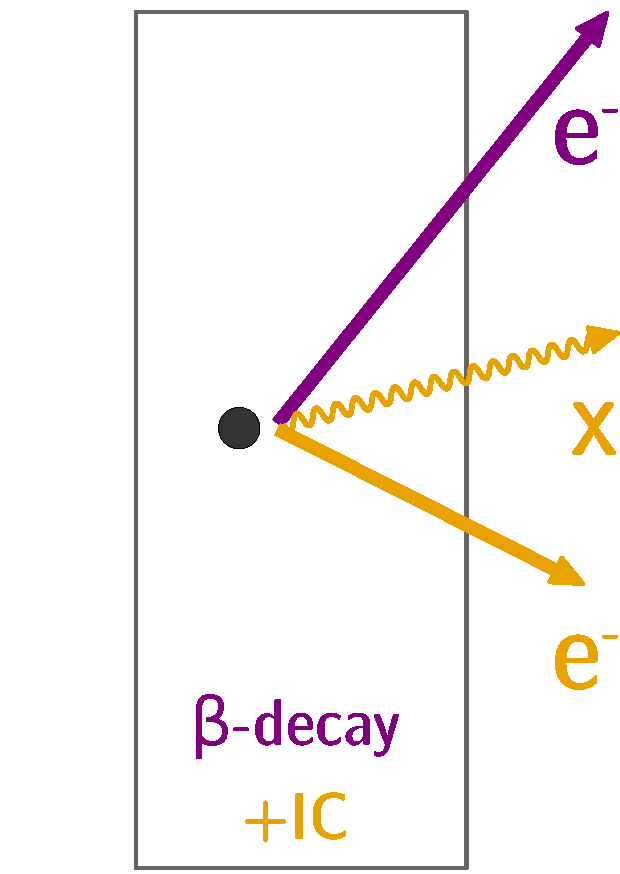
\includegraphics[width=0.82\textwidth]{SNdemonstrator/fig_SNdemonstrator/internal_contamination_IC.pdf}
  \captionsetup{justification=justified}
  \caption{
    \label{subfig:int_cont_IC}}
\end{subfigure}
\hfill
\begin{subfigure}[t]{0.32\textwidth}
  \centering
  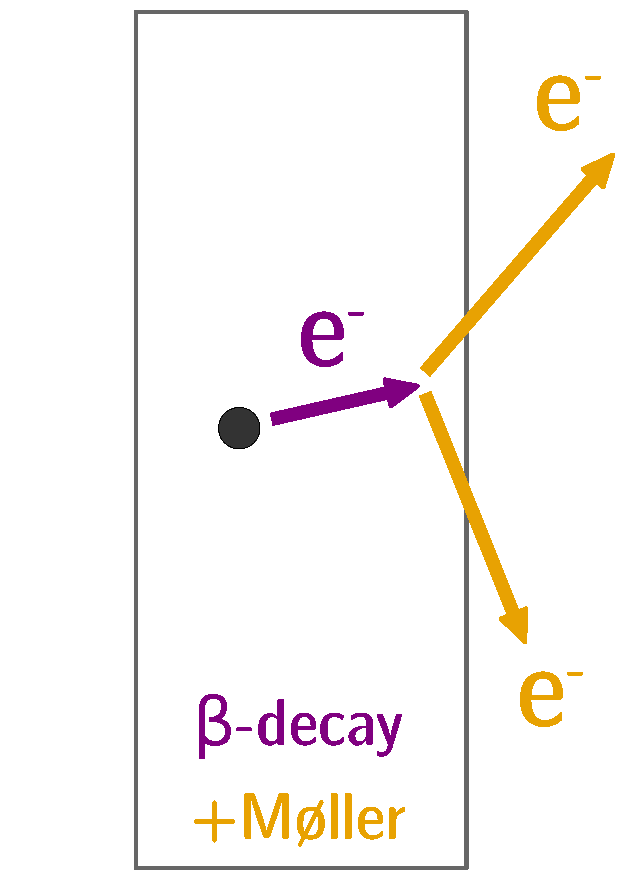
\includegraphics[width=0.82\textwidth]{SNdemonstrator/fig_SNdemonstrator/internal_contamination_moller.pdf}
  \captionsetup{justification=justified}
  \caption{
    \label{subfig:int_cont_moller}}
\end{subfigure}
\hfill
\begin{subfigure}[t]{0.32\textwidth}
  \centering
  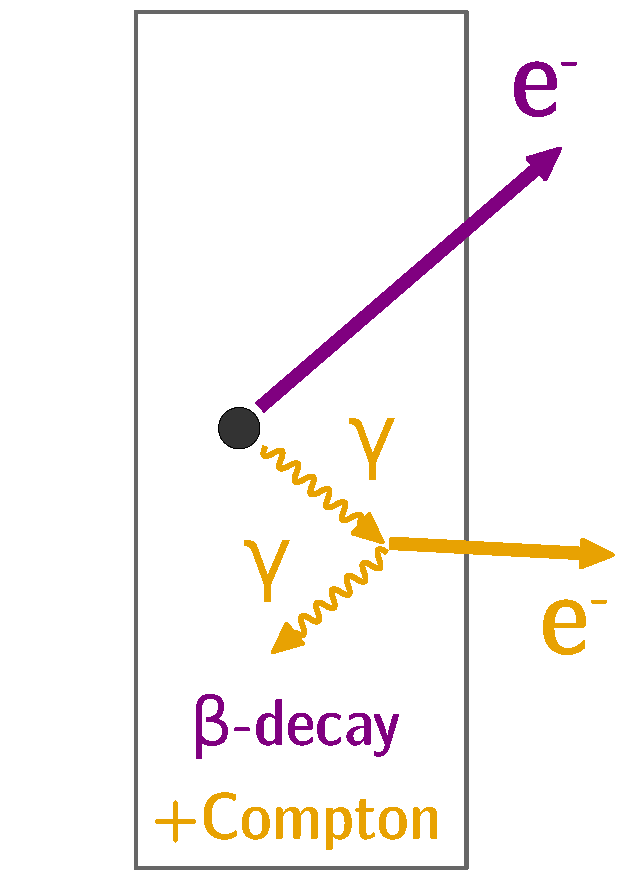
\includegraphics[width=0.82\textwidth]{SNdemonstrator/fig_SNdemonstrator/internal_contamination_compton.pdf}
  \captionsetup{justification=justified}
  \caption{
    \label{subfig:int_cont_compton}}
\end{subfigure}
\caption{(a) $\beta$ decay followed by internal conversion: radioactive nucleus performs a $\beta$ decay, then an electron is emitted after internal conversion of the $\gamma$-ray.
    (b) $\beta$ decay followed by M\o{}ller scattering.
    (c) $\beta$ decay followed by Compton diffusion: radioactive nucleus $\beta$ decays to an excited state, then the photon performs a Compton diffusion.
  \label{fig:internal_contamination}}
\end{figure}

\subsubsection*{Characterisation of background}

The \Tl\ and \Bi\ contaminations inside the source foils are harmful backgrounds for the neutrinoless double beta decay.
One of the key features of the SuperNEMO demonstrator remains its ability to measure its own background in dedicated channels with large statistics, which are independent from the channel used to search for the signal.

After a $\beta$ disintegration, \Tl\ emits between $1$ and $3$ $\gamma$'s.
Consequently, the $1e1\gamma$, $1e2\gamma$ and $1e3\gamma$ channels can be used to discriminate internal \Tl\ events, and measure the activity of the source.
%% However, since the particles share the same fixed energy, the more particles there are, the less energy they will carry.
%% It is therefore less likely for three $\gamma$ to be detected in a short time range, since the half-life times of these levels are very small and the gamma rays pass through the detector.
For \Bi\ disintegrations, between $0$ and $2$ $\gamma$'s are expected after the $\beta$ decay thus a significant contribution to the $1e1\gamma$ channel is also expected from \Bi.
\Bi\ decays via $\beta^{-}$ to $^{214}$Po (the so-called \emph{BiPo events}) which decays via the emission of an $\alpha$ particle with a half-life of $164~\mu$s.
Therefore one can measure BiPo events in the $1e1\alpha(\gamma)$ channel.

\subsubsection*{Internal activities}

The collaboration established recommendations for maximum levels of the internal backgrounds, expressed in number of disintegrations per second, for a unit mass of $\beta\beta$ isotope, or for a unit volume of gas.
These \emph{specified activities} have been calculated in order to achieve the expected sensitivity of the final detector of $\sim 1\times 10^{26}$~years.

The \Se\ demonstrator source is segmented in $34$ foils, whose production was the responsibility of different laboratories (Dubna, LAPP and Tomsk).
The sources have undergone different purification treatments, in order to investigate new techniques, and to compare them with those of NEMO-$3$.
After the sources production and purification, preliminary measurements have been performed with the BiPo-$3$ detector to determine the actual \Tl\ and \Bi\ contamination levels inside the foils~\cite{internal:bipo}.
BiPo-$3$ is a detector installed in the Canfranc underground laboratory in Spain, dedicated to the measurement of the radiopurity in \Tl\ and \Bi\ of NEMO sources before their installation.
It measures the Bismuth-Polonium cascade (electron emission followed by a delayed $\alpha$).
It is made of $2$ modules of $40$ PMs and scintillator blocks each that takes the source foils in sandwich.

We summarise measured contamination levels in Tab.~\ref{tab:real_target_act}, and give a comparison with initial specifications.
The targeted \Tl\ level is not reached, being almost $27$ times higher than expected, and $3.0\times 10^{4}$ internal Thallium events are expected in $2.5$ years in the total energy range.
Nevertheless, on average, the activity of the sources was improved by a factor of $2$ compared to the $^{100}$Mo sources of NEMO-$3$ which is encouraging.
In addition, valuable information has been accumulated on the different production techniques, which are of great importance for the final detector construction.
In particular, the two best \Tl\ sources activities were reached by inverse chromatography, reaching a $20\pm10~\mu$Bq/kg level, an improvement by a factor $5$ compared to NEMO-$3$.
This encourages for further investigations in this direction.
The sensitivity of BiPo-$3$ detector only allowed to give an upper limit on the level of internal \Bi\ (an activity of $290~\mu$Bq/kg would correspond to $1.6\times~10^{5}$ internal Bismuth events in $2.5$ years).
Precise additional measurements are expected from the demonstrator calibration.
\begin{table}[h!]
  \centering
  \begin{tabular}{|c|c|c|}
    \hline
    & Specified activities & Measured activities \\
    \hline\hline
    \Tl  & $2\,\mu$Bq/kg$^{1}$ & $54\,\mu$Bq/kg$^{1}$ [$26$~-~$102$] \\
    \Bi  & $10\,\mu$Bq/kg$^{1}$ & $<290\,\mu$Bq/kg$^{1}$ \\
    \hline
  \end{tabular}
  \caption{Measured and specified activities for the SuperNEMO demonstrator.
    The limit on \Bi\ contamination is provided by BiPo-$3$ measurements for a $90\%$ CL~\cite{internal:bipo}.
    \label{tab:real_target_act}}
\end{table}

\subsection{External background}
\label{subsec:SNexternal_bkg}

\subsubsection*{External background sources}

Different processes originating from outside the detector can mimic $\beta\beta$ decays.
\begin{itemize}
\item External high energy $\gamma$'s emitted after the disintegration of natural radioactive isotopes (mostly \Tl, \Bi\ and \K) occurring outside the detector (typically the lab rocks).
\item Neutrons resulting from the spallation of nuclei by cosmic muons.
\item Contamination of detector materials by natural radioactive nuclei (mostly in PM glass).
\end{itemize}

The three types of processes listed above can be the cause of a photon interaction inside the source and lead to a $\beta\beta$ topology, though different possible processes (Fig.~\ref{fig:external_contamination}).
\begin{itemize}
\item Interaction of such a high-energy photon ($>1.022$~MeV) can induce a creation of an electron/positron pair.
  The presence of a magnetic field in the SuperNEMO experiment allows the discrimination between a positron and an electron thanks to the curvature of their trajectories and thus reduce this background.
\item Two successive Compton scattering can occur, the last gamma escaping detection.
\item After a first Compton scattering, the emitted electron can make a M\o{}ller diffusion on another electron in the source, the gamma being not detected.
\end{itemize}
\begin{figure}[!h]
\centering
\begin{subfigure}[t]{0.32\textwidth}
  \centering
  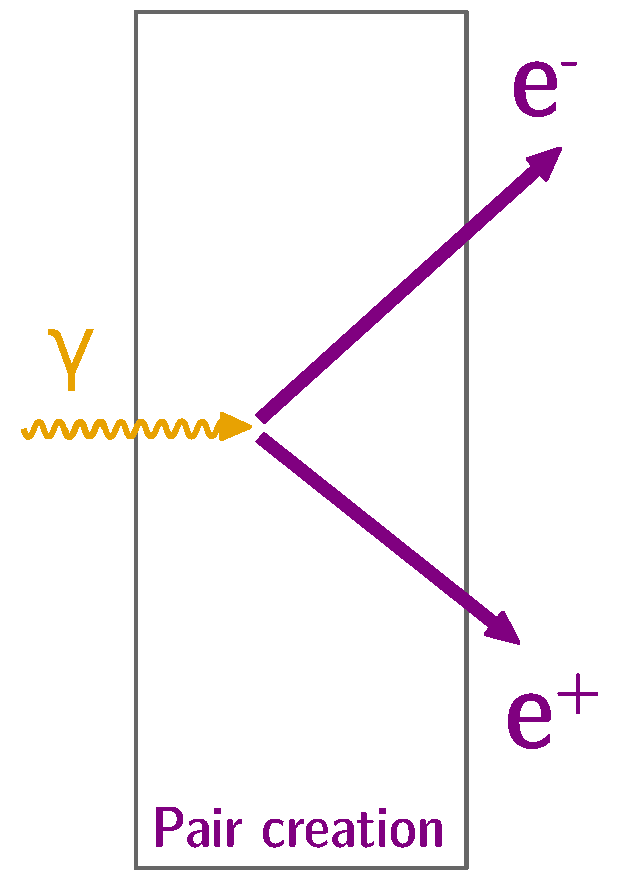
\includegraphics[width=0.82\textwidth]{SNdemonstrator/fig_SNdemonstrator/external_contamination_pair.pdf}
  \captionsetup{justification=justified}
  \caption{
    \label{subfig:ext_cont_pair}}
\end{subfigure}
\hfill
\begin{subfigure}[t]{0.32\textwidth}
  \centering
  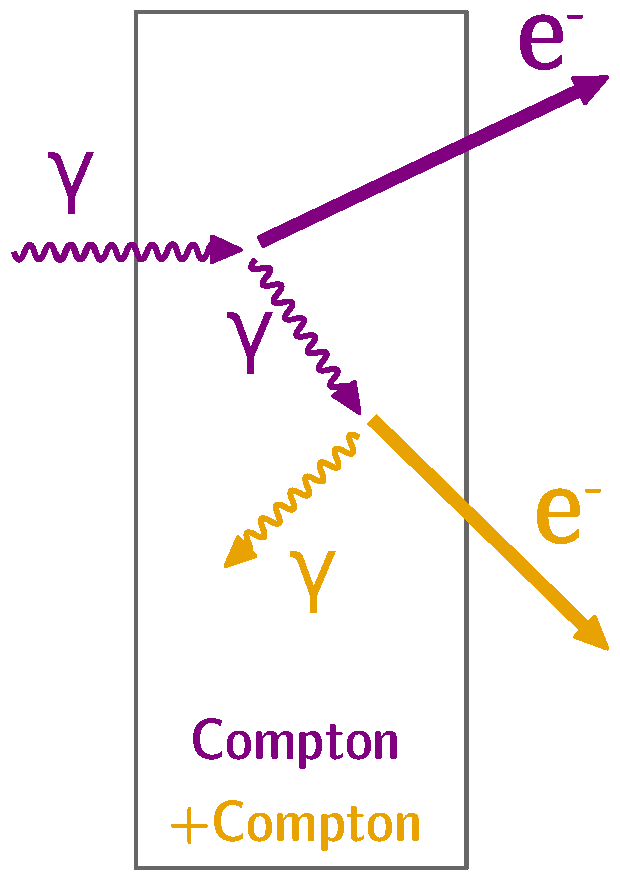
\includegraphics[width=0.82\textwidth]{SNdemonstrator/fig_SNdemonstrator/external_contamination_double_compton.pdf}
  \captionsetup{justification=justified}
  \caption{
    \label{subfig:ext_cont_compton}}
\end{subfigure}
\hfill
\begin{subfigure}[t]{0.32\textwidth}
  \centering
  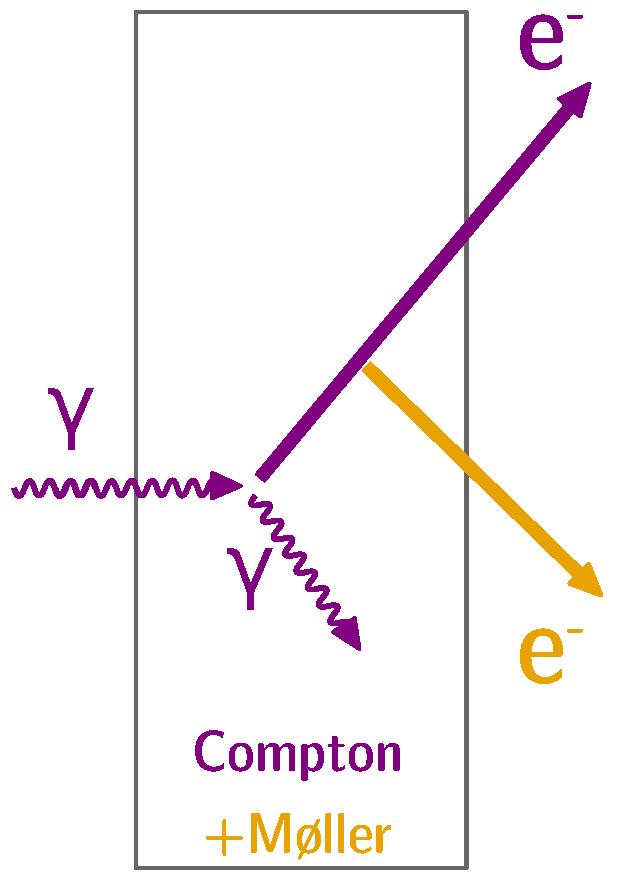
\includegraphics[width=0.82\textwidth]{SNdemonstrator/fig_SNdemonstrator/external_contamination_compton_moller.pdf}
  \captionsetup{justification=justified}
  \caption{
    \label{subfig:ext_cont_moller}}%%arranger ça dans première
\end{subfigure}
\caption{(a) External $\gamma$ undergoes an electron/positron pair creation.
    (b) Two successive Compton scatterings.
  (c) Compton scattering followed by a M\o{}ller scattering.
  \label{fig:external_contamination}}
\end{figure}

\subsubsection*{Radiopurity}

A huge work has been done by Hamamatsu to control the photomultipliers contamination compared with NEMO-$3$, in order to reduce the total radioactive isotope budget for the experiment.
In Tab.~\ref{tab:meas_ext_cont} is presented the total activities measured for $8$ and $5$ inches PMs~\cite{docdb:perrot2017}.
The radiopurity is smaller than for NEMO-$3$ for \K\ and $^{226}$Ra (leading to \Bi\ contamination) by $\sim35$\% but is worse for $^{232}$Th (\Tl) by $\sim150$\%.
\begin{table}[h!]
  \centering
  \begin{tabular}{|c|c|c|c|}
    \hline
    Experiment & \K & $^{226}$Ra & $^{232}$Th \\
    \hline\hline
    SuperNEMO demonstrator~\cite{docdb:perrot2017} & $540$ & $197$ & $124$ \\
    NEMO-$3$~\cite{art:NEMO3_2005} & $832$ & $302$ & $50$ \\
    \hline
  \end{tabular}
  \caption{Total activity in Bq of SuperNEMO and NEMO-$3$ PMs in \K, $^{226}$Ra and $^{232}$Th isotopes.
    \label{tab:meas_ext_cont}}
\end{table}

The NEMO-$3$ experiment set a limit on the external background number of counts, of $<0.2$ events in the $2e$ topology, for the energy range [$2.8$;$3.2$]~MeV (two electrons energy sum), for an exposure of $34.3$ kg·y, with $^{100}$Mo sources~\cite{art:NEMO2015}.
This could lead us to think that the external background contribution for SuperNEMO could be higher than that of NEMO-$3$ because of the higher level of \Tl\ measured.
Hopefully, on that level, the most notorious difference between the two detectors is the fact that the SuperNEMO scintillator blocks are thicker than those of NEMO-$3$.
Therefore, a gamma emitted from a PMT glass is more likely to be detected before crossing the source foils, such that it would be rejected and would not contribute to the background in the $2e$ channel.
Even if the regions of interest are slightly different between these two experiments, it produces a negligible increase on the external background contribution\footnote{A study conducted by the SuperNEMO collaboration showed that at most $0.73$ additional external background events would have been expected for the NEMO-$3$ detector, if instead of taking the [$2.8$;$3.2$]~MeV energy range, we would have considered the [$2.7$;$3.15$]~MeV region of interest.}.%%%%this limit is given by the stat simulated and could be ameliorated by more simulations by CPU


\subsection{Radon background}

Radon is a noble gas which occurs as an indirect decay product of uranium and thorium, which is a daughter of uranium.
Radon contaminations inside the tracker volume is a major background to rare event experiments such as SuperNEMO.
Due to its chemical properties, radon has a long diffusion length in solids, making it difficult to remove.
This isotope is outgased in the surrounding air from the rock walls of the laboratory and detector materials and can enter the detector.
The potential sources of radon are
\begin{itemize}
\item gas contamination at the tracker entrance,
\item emanation of the tracker materials,
\item radon diffusion from the detector material to the tracker,
\item radon diffusion from the laboratory to the tracker.
\end{itemize}

Simulations show that, to achieve the designed sensitivity for the final SuperNEMO detector, the level of radon must not exceed $0.15$ mBq/m$^{3}$ since its decay daughter \Bi\ can mimic a $\zeronu$ event.
The level of radon emissions inside the tracker was extrapolated by the collaboration for each of the four C-section, revealing an expected total activity of $0.15\pm0.02$ mBq/m$^{3}$ ($67$\% CL), assuming the combination of an anti-radon tent and an air-flushing method ($2$~m$^{3}$/h gas flow rate)~\cite{conf:radon2017}.
These levels were measured using a concentration line where the detector materials are enclosed in a chamber in which they emanate Radon.
The gas from the vessel is then sent to a Radon trap in order to measure the concentration of this isotope.


\subsection{Background reduction}
\label{subsec:background_reduc}

\subsubsection*{The underground laboratory}

The LSM is located under the Fréjus mountain besides the road tunnel of the same name that links France and Italy.
This laboratory is one of the deepest in the world with a maximal rock thickness of $1700$~m, or $4800$ meter water equivalent.
At this depth, the flow of cosmic muons is reduced by a $10^{6}$ compared to the surface (the muon flux is measured at $\sim4$~muons/m$^{2}$/day in the laboratory).

\subsubsection*{External shield}

In order to reduce the contribution of external gamma background, ultra-pure iron plates $20$~cm thick form a shield surrounding the anti-radon tent.
In addition,the detector will be protected from neutrons by a final shield consisting of water tanks (on the sides of the detector) and borated Polyethylene plates (top and bottom).

\subsubsection*{Radon background reduction}

A wide variety of means are employed by the collaboration to combat this contamination.
\begin{itemize}
\item Radon trap: the gas in the tracker is constantly recycled.
  On this occasion, the gas (without ethanol) is sent into a radon trap before being re-injected into the tracker.
\item The emanations of the tracker materials were measured in Manchester with the concentration line before the installation of the chambers.
\item The gas flow can be reasonably increased to have a sufficiently low Radon level.
\item The huge effort deployed for the detector gas tightness (Sec.~\ref{subsec:sealing}) is one of the means to reduce radon contamination.
\item The detector will be encapsulated in its entirety in a Radon Tent made of High Density Polyethylene (HDPE) panels preventing radon from the laboratory from entering the detector by possible tiny gaps.
\end{itemize}


\section{The SuperNEMO software}
\label{sec:SNsoftware}

The SuperNEMO collaboration developed its own simulation, reconstruction and analysis environment.
The Falaise software, specifically designed by and for the SuperNEMO collaboration, holds the \verb!C++! library for the event reconstruction and analysis of simulated and real data.
Especially, it contains the geometry, the detector material, the event data model, the reconstruction algorithms and the data analysis.
Finally, the SNFee software is a tool package for the configuration, control and monitoring of the SuperNEMO front-end electronics.


\subsection{Simulation}

The Falaise software handles the simulation of events based on the Monte-Carlo method implemented in GEANT$4$.
The event generation, the detector geometry and its materials are simulated.
The process to be simulated ($\twonu$, radioactive isotope decays...), its location (source foils, PM glass...), as well as the detector configuration (on/off magnetic field, presence or absence of external shield...) can be set by using configuration files.
After the Monte-Carlo simulations, the detector performances and characteristics (optical module energy resolutions, Geiger cell spatial resolution...) are implemented in order to reproduce the behaviour of the detector as faithfully as possible.


\subsection{Reconstruction pipeline}

The Falaise Software of SuperNEMO is made up of successive algorithms allowing to characterise the events stored after a data acquisition or a simulation.
\paragraph{} The tracker clustering is in charge of clustering individual Geiger cell hits to form continuous traces and thus identify the number of charged particles of an event.
\paragraph{} The tracker trajectory fitting fits the reconstructed traces with two patterns: a helix (well adapted to the identification of electrons and positrons of a few MeV that have a curved trajectory in the magnetic field of the experiment) and with a line (rather adapted to muons and alpha particles).
The fit with the best $\chi^{2}/ndf$ is then selected.
\paragraph{} The charged particle tracking: previous algorithms are suitable for any experience with a thread chamber.
The present one adapts informations to the SuperNEMO specific geometry.
It extrapolates the charged particles trajectories to associate a calorimeter block and a source foil vertex to each track.
\paragraph{} The gamma clustering: as gamma particles do not interact inside the tracker, the tracker clustering algorithm does not handle such particles.
After the charged particle tracking algorithm, some calorimeter hits remain not associated with any track.
The gamma clustering algorithm is dedicated to reconstruct the successive diffusions of gammas in scintillators using geometrical and time-of-flight informations.
\paragraph{} The particle identification (PID): all previous algorithms have permitted the individual reconstruction of the different particles of an event.
The particle identification module takes care of identifying and classify each particle as:
\begin{itemize}
\item Electron: negatively curved track with an associated calorimeter hit and a vertex on the source foil.
\item Positron: positively curved track with an associated calorimeter hit and a vertex on the source foil.
\item Alpha particle: short straight track with possible time delay.
\item Gamma particle: unassociated calorimeter hit.
\end{itemize}
This last algorithm is not yet included in the official Falaise pipeline but were nonetheless widely used in the framework of the two analyses presented in Chapters~\ref{ch:sensitivity} and~\ref{ch:timediff}.

The SuperNEMO software also provides a high precision visualisation, of which an example is given in Fig.~\ref{fig:visu}.
One electron and two $\gamma$'s are simulated then reconstructed.
One of the $\gamma$ scatters in a first scintillator and deposits energy in a second one.
\begin{figure}[h!]
\centering
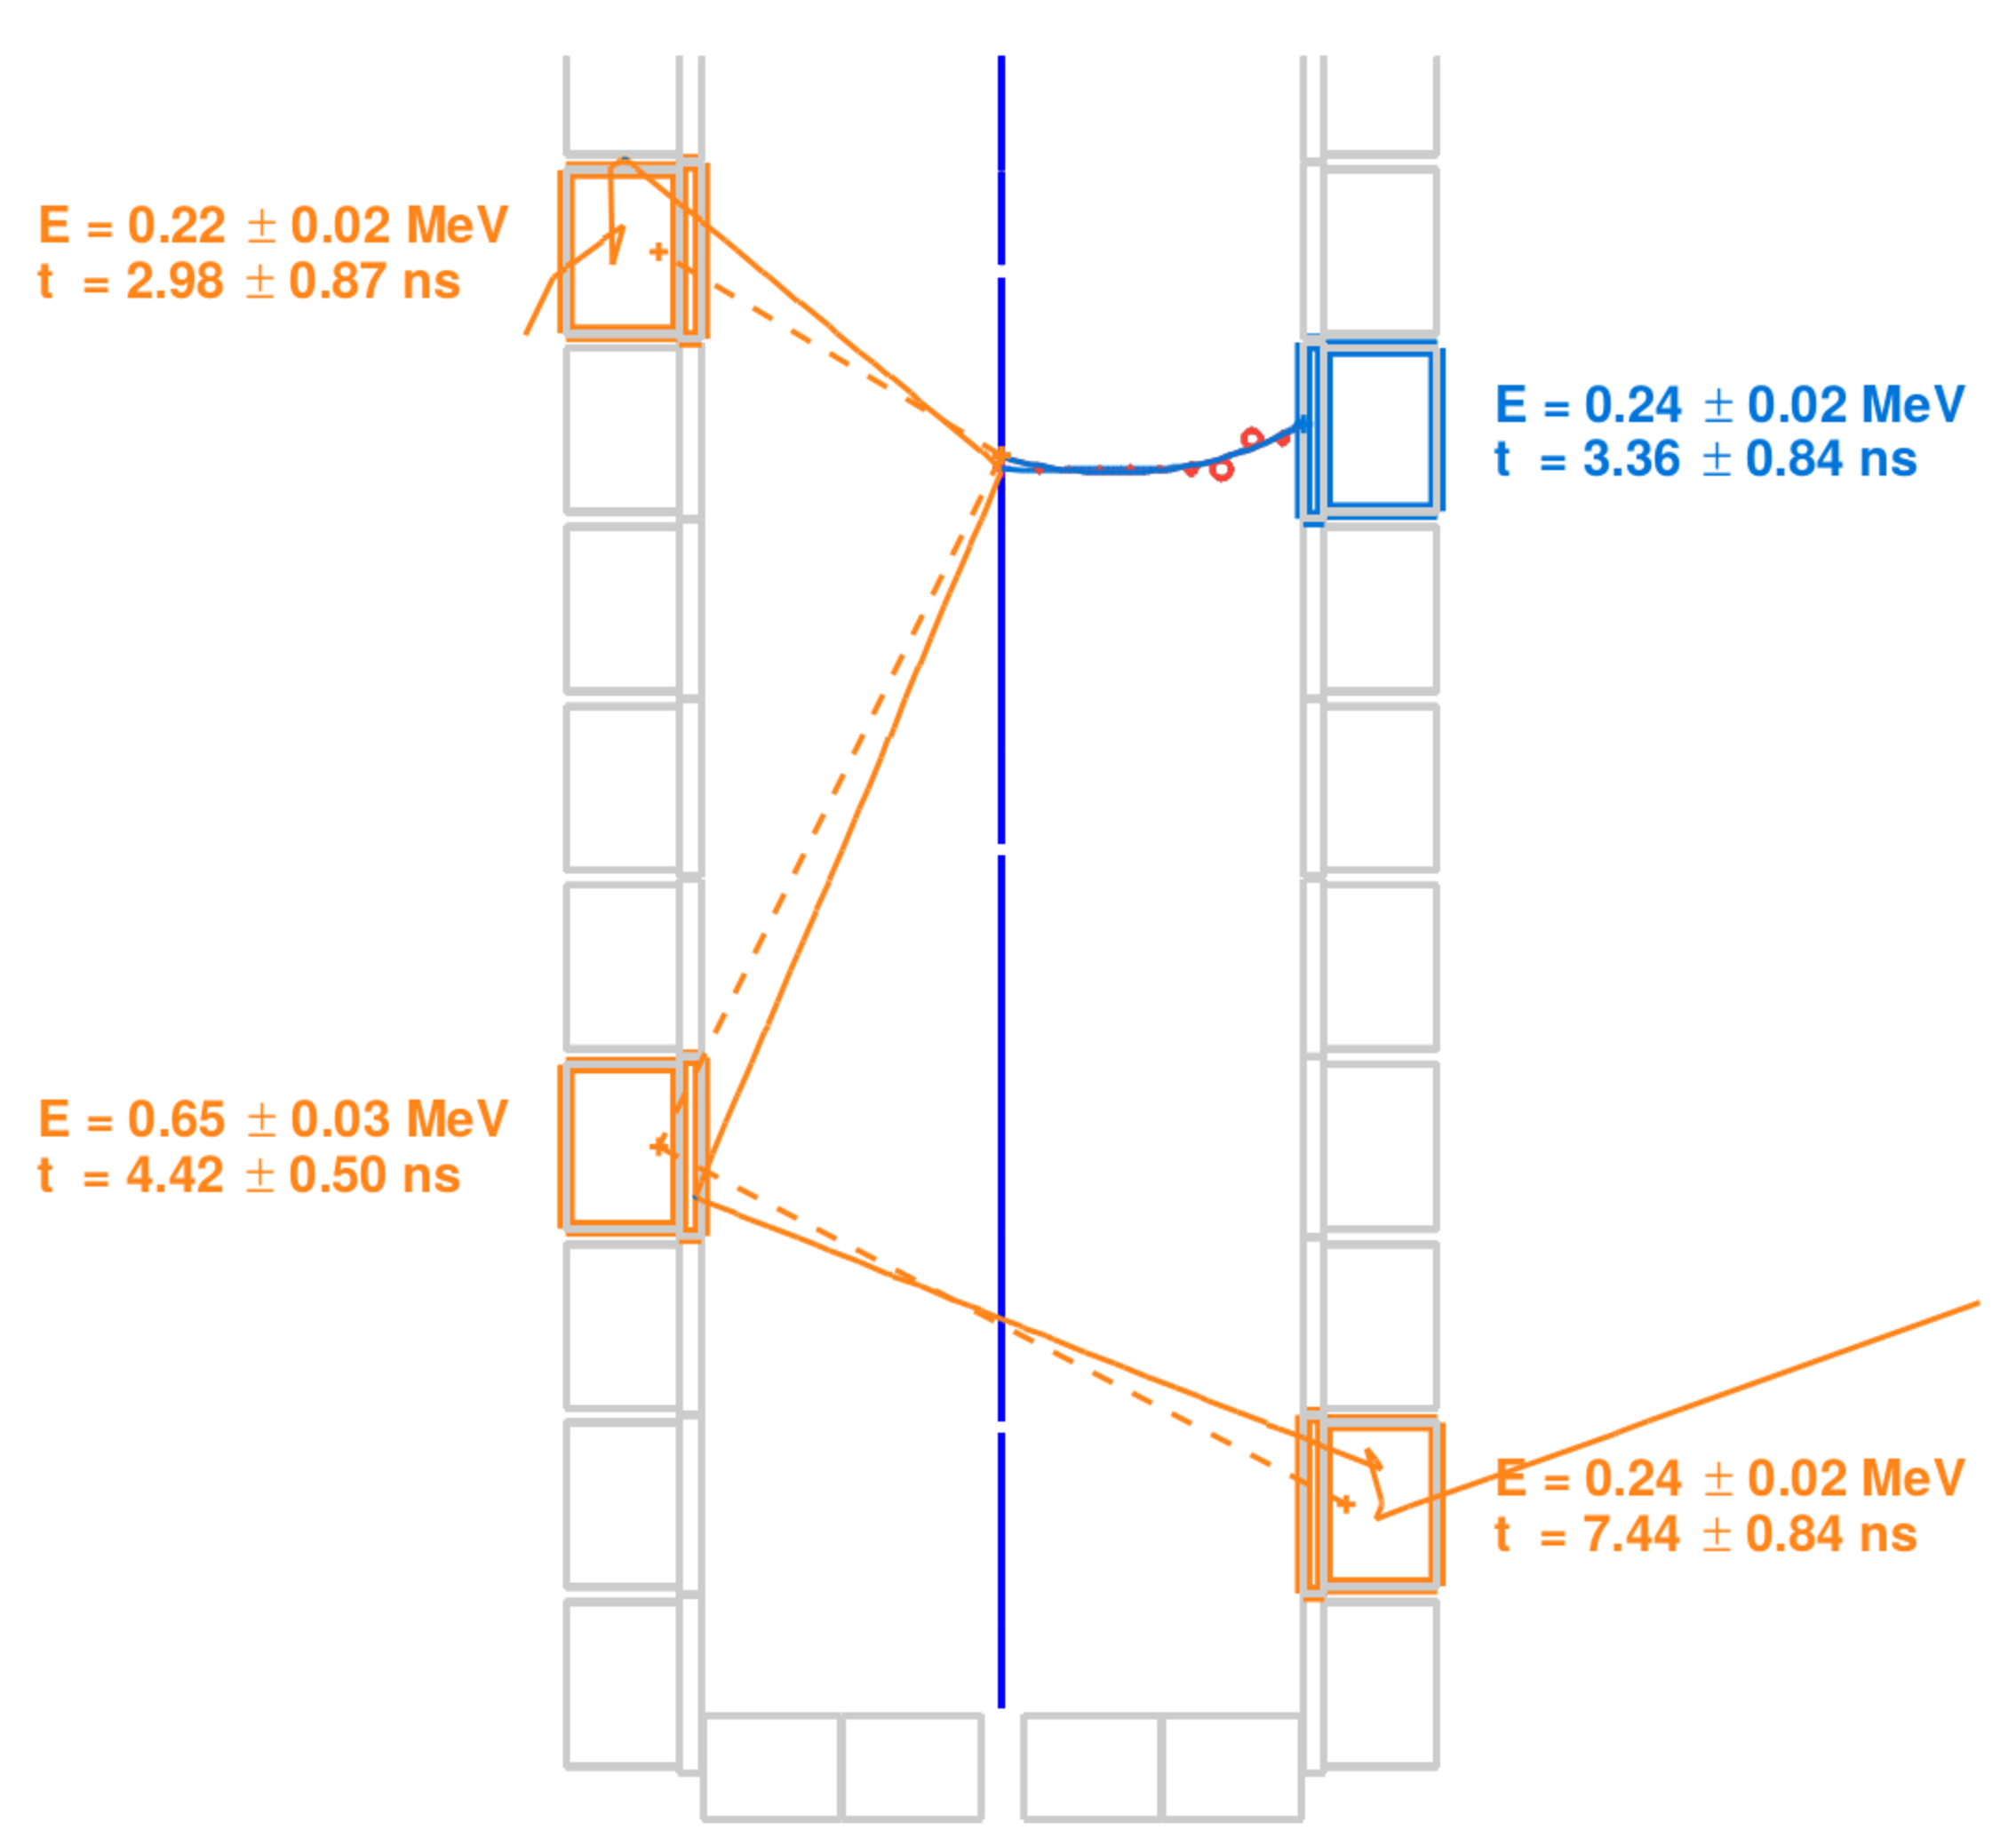
\includegraphics[width=0.7\textwidth]{SNdemonstrator/fig_SNdemonstrator/Falaise_visu.pdf}
\caption{Display of an event with one electron (blue) and two $\gamma$'s (orange) emitted.
  The simulated tracks are solid lines and reconstructed are dashed lines.
  The visualisation is provided by the Falaise software.
\label{fig:visu}}
\end{figure}


\subsection{Analysis tools}
\label{subsec:analysis_tools}

Internal and external probabilities are extremely useful tools, widely employed in particular by the gamma clustering algorithm and particle identification module.
They are also used for analysis purposes, to determine whether or not an event does come from inside or outside the source foils.

\subsubsection{Internal probability}
\label{subsec:internal_prob}

Internal probability is a mathematical tool used to quantify the probability that two particles were emitted simultaneously in the source foils.
This tool is based on the particle Time-Of-Flight computation.
%and this measurement can only be performed if both particles have at least one associated calorimeter hit, and that one of them is charged (a vertex is needed to formulate a hypothesis.)
Firstly, we define, for two particles, the internal $\chi^{2}$
\begin{equation}
  \chi^{2}_{int}=\frac{((t^{meas}_{1} - t^{exp}_{1}) - (t^{meas}_{2} - t^{exp}_{2}))^{2}}{\sigma_{tot}^{2}}\,.
  \label{eq:int_chi2}
\end{equation}
$t^{exp}_{i}$ is the expected time-of-flight of the particle $i$ inside the calorimeter, $t^{meas}_{i}$ the measured one, c is the speed of light, and $\sigma_{tot}$ is the quadratic sum of all uncertainties.
The expected time-of-flight, is defined as
\begin{equation}
  t^{exp}_{i}=\frac{L_{i}}{\beta_{i}\,c}\,,
  \label{eq:th_time}
\end{equation}
where $L_{i}$ is the reconstructed track length, and $\beta_{i}$ corresponds to
\begin{equation}
  \beta_{i}=\frac{\sqrt{E_{i}(E_{i} + 2m_{i})}}{E_{i} + m_{i}}\,,
  \label{eq:beta_i}
\end{equation}
$E_{i}$ being the energy of the particle and $m_{i}$ its mass.
The total uncertainty, $\sigma_{tot}$, is defined as
\begin{equation}
  \sigma_{tot}=\sqrt{\sigma_{t_{1}}^{2}+\sigma_{t_{2}}^{2}+\sigma_{\beta_{2}}^{2}+\sigma_{\beta_{1}}^{2}+\sigma_{l_{1}}^{2}+\sigma_{l_{2}}^{2}} \,.
  \label{eq:sigma_tot}
\end{equation}

\paragraph{The uncertainty $\sigma_{t}$ on the measured time-of-fight}
This term is directly related to the phenomenon of absorption and re-emission of scintillation photons, as well as to the photomultiplier functioning.
It is defined as
\begin{equation}
  \sigma_{t}=\sqrt{\dfrac{\tau_{\text{SC}}^{2}+\left(\dfrac{\text{FWHM}_{\text{TTS}}}{2\sqrt{2\ln{2}}}\right)^{2}}{\text{N}_\text{PE}}}\,,
  \label{eq:sigma_t}
\end{equation}
where $\tau_{\text{SC}}$ is the scintillator characteristic time representing the scintillator de-excitation time.
$\text{FWHM}_{\text{TTS}}$ is the temporal dispersion linked to the photomultiplier: the transit time of the photoelectrons inside the photomultiplier can evolve, according to its point of creation on the photocathode.
This transit time is unique for each photomultiplier, and has to be characterised experimentally.
$\text{N}_\text{PE}$ is the number of photo-electrons emitted after a particle has deposited all its energy $E$ in the scintillator:
\begin{equation}
  \text{N}_\text{PE} = E\times \left(\frac{2\sqrt{2\ln 2}}{\text{FWHM}_{\text{E}}}\right)^{2}\,,
\end{equation}
where $\text{FWHM}_{\text{E}}$ is the energy resolution of the PM, $8~\%$ at $1$~MeV for the SuperNEMO calorimeter.
Therefore, for a particle of $1$~MeV depositing all its energy inside a scintillator, $\text{N}_\text{PE}\sim 866$ photo-electrons are emitted.
Preliminary studies gave a first estimation of $\sigma_{t}$ and found $\sigma_{t}=342\pm 10$~ps for $1$~MeV gammas entering the front face of the scintillator, and $\sigma_{t}=248\pm 6$~ps for $1$~MeV electrons~\cite{HuberThesis}.
On the occasion of the SuperNEMO detector commissioning, we complete this study and characterise the calorimeter time resolution in Chapter~\ref{ch:Cobalt_study}.

\paragraph{The uncertainty $\sigma_{\beta}$ on the expected time-of-flight induced by the uncertainty on the particle energy}
This term is derived from Eqs.~\eqref{eq:th_time}~and~\eqref{eq:beta_i}:
\begin{equation}
%% \sigma_{\beta_{i}} = \biggl\lvert \dfrac{\partial t^{exp}_{i}}{\partial E_{i}}  \biggr\rvert
  %% \Delta E_{i}\,,
  \sigma_{\beta_{i}} = \frac{t^{exp}_{i}\times m_{i}^{2}}{E_{i}\times (E_{i}+m_{i})\times (E_{i}+2m_{i})}\times \sigma_{E}\,,
  \label{eq:sigma_L}
\end{equation}
where $\sigma_{E}= \text{FWHM}_{\text{E}} \times \sqrt{E_{i}}$ represents the energy resolution of the PM for the energy $E_{i}$.

\paragraph{The uncertainty $\sigma_{l}$ on the expected time induced by the uncertainty on the reconstructed track length}
This corresponds to the typical uncertainty due to particle track reconstruction.
It is induced mainly by the uncertainty on the interaction point inside the scintillator block, thus is greater for $\gamma$ particles than for electrons.
Indeed, thanks to the gaseous detector and the trajectory fitting, valuable information on the impact point inside the scintillator are provided for electrons crossing the tracker, while photons only deposit their energy inside the calorimeter, without ionising the tracker gas.
In the framework of the optimisation of $\gamma$ reconstruction in the SuperNEMO detector, a previous study has evaluated the uncertainty on the track length for $\gamma$'s, by simulating mono-kinetic $\gamma$'s, and estimated $\sigma_{L}=0.9$~ns~\cite{CalvezThesis}.
The value used in the simulation/reconstruction pipeline, for the case of electrons, is inherited from the NEMO-$3$ analysis with $\sigma_{L}=0.1$~ns.
An optimisation of this parameter is given in Chapter~\ref{ch:timediff}.

\paragraph{}

We would translate the internal $\chi^{2}$ distribution into the so-called \emph{internal probability} through
\begin{equation}
  %%P_{int} = \frac{1}{2\pi}\int_{\chi^{2}_{int}}^{+\infty}x^{-\frac{1}{2}}e^{-\frac{x}{2}}dx\,. %%sans changement variable
  P_{int} = \frac{2}{\sqrt{2\pi}}\int_{\chi_{int}}^{+ \infty} e^{-\frac{u^{2}}{2}} du %% avec changement variable
  %%P_{int} = erfc\left(\sqrt{\frac{\chi^{2}_{int}}{2}}\right)\,.
  \label{eq:chi2_Pint}
\end{equation}
This formula transforms the $\chi^{2}$ Gaussian distribution into a flat distribution between $0$ and $1$.
One of the benefits of using the probability distribution rather than the $\chi^{2}$ distribution is that it brings extra qualitative information, especially useful to check the estimation of the uncertainties.
The shape of the probability distribution can bring out an overestimation or an underestimation of the uncertainties, which would translate into a positive or a negative slope, respectively.
On the other hand, a flat distribution signifies an appropriate estimation of the errors and confirms the Gaussian distribution of the original quantity measured.

%% As explained earlier, the probability distribution is obtained from a transformation of the χ2 distribution.
%% If the errors involved in the computation of the latter are aptly estimated, the χ2 should follow a Gaussian distribution, simply generated by the limited time and energy resolution of the detector.


\subsubsection{External probability}

The external probability is built to test if one of the two particles (electron, $\gamma$) first deposited energy in the calorimeter, crossed the tracker to reach the source foil and triggered a second calorimeter module (with or without interacting inside the source foils when crossing it).
The external $\chi^{2}$ is defined in the same manner as the internal one:
\begin{equation}
  \chi^{2}_{int}=\frac{(|t^{meas}_{1} - t^{meas}_{2}| - (t^{exp}_{1} + t^{exp}_{2}))^{2}}{\sigma_{tot}^{2}}\,.
  \label{eq:ext_chi2}
\end{equation}
The time experimental difference is compared to the time it would have taken a particle to travel from one calorimeter module to the other.
The external $\chi^{2}$ is translated into the so-called \emph{external probability} the same way as in Eq.~\eqref{eq:chi2_Pint}.

\section{Summary}

SuperNEMO demonstrator features have been exposed, and often compared with the ones of its predecessor, NEMO-$3$.
This detector aims at demonstrating that the NEMO unique technology is scalable in order to explore previously unattained reaches in the search for the $\zeronu$ decay.
Previous studies have been led in order to estimate the sensitivity of SuperNEMO to this decay.
The one presented in the next chapter follows them by evaluating the influence of several parameters.

The detector calibration has started and should be completed this year thanks to the involvement of all the collaboration.
